\RequirePackage[l2tabu, orthodox]{nag}
\documentclass[version=3.21, pagesize, twoside=off, bibliography=totoc, DIV=calc, fontsize=12pt, a4paper]{scrartcl}
%Permits to copy eg x ⪰ y ⇔ v(x) ≥ v(y) from PDF to unicode data, and to search. From pdfTeX users manual. See https://tex.stackexchange.com/posts/comments/1203887.
	\input glyphtounicode
	\pdfgentounicode=1
%Latin Modern has more glyphs than Computer Modern, such as diacritical characters. fntguide commands to load the font before fontenc, to prevent default loading of cmr.
	\usepackage{lmodern}
%Encode resulting accented characters correctly in resulting PDF, permits copy from PDF.
	\usepackage[T1]{fontenc}
%UTF8 seems to be the default in recent TeX installations, but not all, see https://tex.stackexchange.com/a/370280.
	\usepackage[utf8]{inputenc}
%Provides \newunicodechar for easy definition of supplementary UTF8 characters such as → or ≤ for use in source code.
	\usepackage{newunicodechar}
%Text Companion fonts, much used together with CM-like fonts. Provides \texteuro and commands for text mode characters such as \textminus, \textrightarrow, \textlbrackdbl.
	\usepackage{textcomp}
%St Mary’s Road symbol font, used for ⟦ = \llbracket.
	\usepackage{stmaryrd}
%Solves bug in lmodern, https://tex.stackexchange.com/a/261188; probably useful only for unusually big font sizes; and probably better to use exscale instead. Note that the authors of exscale write against this trick.
	%\DeclareFontShape{OMX}{cmex}{m}{n}{
		%<-7.5> cmex7
		%<7.5-8.5> cmex8
		%<8.5-9.5> cmex9
		%<9.5-> cmex10
	%}{}
	%\SetSymbolFont{largesymbols}{normal}{OMX}{cmex}{m}{n}
%More symbols (such as \sum) available in bold version, see https://github.com/latex3/latex2e/issues/71.
	\DeclareFontShape{OMX}{cmex}{bx}{n}{%
	   <->sfixed*cmexb10%
	   }{}
	\SetSymbolFont{largesymbols}{bold}{OMX}{cmex}{bx}{n}
%For small caps also in italics, see https://tex.stackexchange.com/questions/32942/italic-shape-needed-in-small-caps-fonts, https://tex.stackexchange.com/questions/284338/italic-small-caps-not-working.
	\usepackage{slantsc}
	\AtBeginDocument{%
		%“Since nearly no font family will contain real italic small caps variants, the best approach is to substitute them by slanted variants.” -- slantsc doc
		%\DeclareFontShape{T1}{lmr}{m}{scit}{<->ssub*lmr/m/scsl}{}%
		%There’s no bold small caps in Latin Modern, we switch to Computer Modern for bold small caps, see https://tex.stackexchange.com/a/22241
		%\DeclareFontShape{T1}{lmr}{bx}{sc}{<->ssub*cmr/bx/sc}{}%
		%\DeclareFontShape{T1}{lmr}{bx}{scit}{<->ssub*cmr/bx/scsl}{}%
	}
%Warn about missing characters.
	\tracinglostchars=2
%Nicer tables: provides \toprule, \midrule, \bottomrule.
	%\usepackage{booktabs}
%For new column type X which stretches; can be used together with booktabs, see https://tex.stackexchange.com/a/97137. “tabularx modifies the widths of the columns, whereas tabular* modifies the widths of the inter-column spaces.” Loads array.
	%\usepackage{tabularx}
%math-mode version of "l" column type. Requires \usepackage{array}.
	%\usepackage{array}
	%\newcolumntype{L}{>{$}l<{$}}
%Provides \xpretocmd and loads etoolbox which provides \apptocmd, \patchcmd, \newtoggle… Also loads xparse, which provides \NewDocumentCommand and similar commands intended as replacement of \newcommand in LaTeX3 for defining commands (see https://tex.stackexchange.com/q/98152 and https://github.com/latex3/latex2e/issues/89).
	\usepackage{xpatch}
%ntheorem doc says: “empheq provides an enhanced vertical placement of the endmarks”; must be loaded before ntheorem. Loads the mathtools package, which loads and fixes some bugs in amsmath and provides \DeclarePairedDelimiter. amsmath is considered a basic, mandatory package nowadays (Grätzer, More Math Into LaTeX).
	\usepackage[ntheorem]{empheq}
%Package frenchb asks to load natbib before babel-french. Package hyperref asks to load natbib before hyperref.
	\usepackage{natbib}

\newtoggle{LCpres}
	\newtoggle{LCart}
	\newtoggle{LCposter}
	\makeatletter
	\@ifclassloaded{beamer}{
		\toggletrue{LCpres}
		\togglefalse{LCart}
		\togglefalse{LCposter}
		\wlog{Presentation mode}
	}{
		\@ifclassloaded{tikzposter}{
			\toggletrue{LCposter}
			\togglefalse{LCpres}
			\togglefalse{LCart}
			\wlog{Poster mode}
		}{
			\toggletrue{LCart}
			\togglefalse{LCpres}
			\togglefalse{LCposter}
			\wlog{Article mode}
		}
	}
	\makeatother%

%Language options ([french, english]) should be on the document level (last is main); except with tikzposter: put [french, english] options next to \usepackage{babel} to avoid warning. beamer uses the \translate command for the appendix: omitting babel results in a warning, see https://github.com/josephwright/beamer/issues/449. Babel also seems required for \refname.
	\iftoggle{LCpres}{
		\usepackage{babel}
	}{
	}
	%\frenchbsetup{AutoSpacePunctuation=false}
%listings (1.7) does not allow multi-byte encodings. listingsutf8 works around this only for characters that can be represented in a known one-byte encoding and only for \lstinputlisting. Other workarounds: use literate mechanism; or escape to LaTeX (but breaks alignment).
	%\usepackage{listings}
	%\lstset{tabsize=2, basicstyle=\ttfamily, escapechar=§, literate={é}{{\'e}}1}
%I favor acro over acronym because the former is more recently updated (2018 VS 2015 at time of writing); has a longer user manual (about 40 pages VS 6 pages if not counting the example and implementation parts); has a command for capitalization; and acronym suffers a nasty bug when ac used in section, see https://tex.stackexchange.com/q/103483 (though this might be the fault of the silence package and might be solved in more recent versions, I do not know) and from a bug when used with cleveref, see https://tex.stackexchange.com/q/71364. However, loading it makes compilation time (one pass on this template) go from 0.6 to 1.4 seconds, see https://bitbucket.org/cgnieder/acro/issues/115. Option short-format not usable in the package options as it is fragile, see https://tex.stackexchange.com/q/466882.
	%\usepackage[single]{acro}
	%\acsetup{short-format = {\scshape}}
	%\DeclareAcronym{AMCD}{short=amcd, long={Aide Multicritère à la Décision}}
\DeclareAcronym{AR}{short=ar, long={Argumentative Recommender}}
\DeclareAcronym{DA}{short=da, long={Decision Analysis}}
\DeclareAcronym{DJ}{short=dj, long={Deliberated Judgment}}
\DeclareAcronym{DM}{short=dm, long={Decision Maker}}
\DeclareAcronym{DP}{short=dp, long={Deliberated Preference}}
\DeclareAcronym{MAVT}{short=mavt, long={Multiple Attribute Value Theory}}
\DeclareAcronym{MCDA}{short=mcda, long={Multicriteria Decision Aid}}
\DeclareAcronym{MIP}{short=mip, long={Mixed Integer Program}}


\iftoggle{LCpres}{
	%I favor fmtcount over nth because it is loaded by datetime anyway; and fmtcount warns about possible conflicts when loaded after nth.
	\usepackage{fmtcount}
	%For nice input of date of presentation. Must be loaded after the babel package. Has possible problems with srcletter: https://golatex.de/verwendung-von-babel-und-datetime-in-scrlttr2-schlaegt-fehlt-t14779.html.
	\usepackage[nodayofweek]{datetime}
}{
}
%For presentations, Beamer implicitely uses the pdfusetitle option. ntheorem doc says to load hyperref “before the first use of \newtheorem”. autonum doc mandates option hypertexnames=false. I want to highlight links only if necessary for the reader to recognize it as a link, to reduce distraction. In presentations, this is already taken care of by beamer (https://tex.stackexchange.com/a/262014). If using colorlinks=true in a presentation, see https://tex.stackexchange.com/q/203056. Crashes the first compilation with tikzposter, just compile again and the problem disappears, see https://tex.stackexchange.com/q/254257.
\makeatletter
\iftoggle{LCpres}{
	\usepackage{hyperref}
}{
	\usepackage[hypertexnames=false, pdfusetitle, linkbordercolor={1 1 1}, citebordercolor={1 1 1}, urlbordercolor={1 1 1}]{hyperref}
	%https://tex.stackexchange.com/a/466235
	\pdfstringdefDisableCommands{%
		\let\thanks\@gobble
	}
}
\makeatother
%urlbordercolor is used both for \url and \doi, which I think shouldn’t be colored, and for \href, thus might want to color manually when required. Requires xcolor.
	\NewDocumentCommand{\hrefblue}{mm}{\textcolor{blue}{\href{#1}{#2}}}
%hyperref doc says: “Package bookmark replaces hyperref’s bookmark organization by a new algorithm (...) Therefore I recommend using this package”.
	\usepackage{bookmark}
%Need to invoke hyperref explicitly to link to line numbers: \hyperlink{lintarget:mylinelabel}{\ref*{lin:mylinelabel}}, with \ref* to disable automatic link. Also see https://tex.stackexchange.com/q/428656 for referencing lines from another document.
	%\usepackage{lineno}
	%\NewDocumentCommand{\llabel}{m}{\hypertarget{lintarget:#1}{}\linelabel{lin:#1}}
	%\setlength\linenumbersep{9mm}
%For complex authors blocks. Seems like authblk wants to be later than hyperref, but sooner than silence. See https://tex.stackexchange.com/q/475513 for the patch to hyperref pdfauthor.
	\ExplSyntaxOn
	\seq_new:N \g_oc_hrauthor_seq
	\NewDocumentCommand{\addhrauthor}{m}{
		\seq_gput_right:Nn \g_oc_hrauthor_seq { #1 }
	}
	%Should be \NewExpandableDocumentCommand, but this is not yet provided by my version of xparse
	\DeclareExpandableDocumentCommand{\hrauthor}{}{
		\seq_use:Nn \g_oc_hrauthor_seq {,~}
	}
	\ExplSyntaxOff
	{
		\catcode`#=11\relax
		\gdef\fixauthor{\xpretocmd{\author}{\addhrauthor{#2}}{}{}}%
	}
	\iftoggle{LCart}{
		\usepackage{authblk}
		\renewcommand\Affilfont{\small}
		\fixauthor
		\AtBeginDocument{
		    \hypersetup{pdfauthor={\hrauthor}}
		}
	}{
	}
%I do not use floatrow, because it requires an ugly hack for proper functioning with KOMA script (see scrhack doc). Instead, the following command centers all floats (using \centering, as the center environment adds space, http://texblog.net/latex-archive/layout/center-centering/), and I manually place my table captions above and figure captions below their contents (https://tex.stackexchange.com/a/3253).
	\makeatletter
	\g@addto@macro\@floatboxreset\centering
	\makeatother
%Permits to customize enumeration display and references
	%\nottoggle{LCpres}{
		%\usepackage{enumitem} %follow list environments by a string to customize enumeration, example: \begin{description}[itemindent=8em, labelwidth=!] or \begin{enumerate}[label=({\roman*}), ref={\roman*}].
	%}{
	%}
%Provides \Centering, \RaggedLeft, and \RaggedRight and environments Center, FlushLeft, and FlushRight, which allow hyphenation. With tikzposter, seems to cause 1=1 to be printed in the middle of the poster.
	%\usepackage{ragged2e}
%To typeset units by closely following the “official” rules.
	%\usepackage[strict]{siunitx}
%Turns the doi provided by some bibliography styles into URLs. However, uses old-style dx.doi url (see 3.8 DOI system Proxy Server technical details, “Users may resolve DOI names that are structured to use the DOI system Proxy Server (https://doi.org (current, preferred) or earlier syntax http://dx.doi.org).”, https://www.doi.org/doi_handbook/3_Resolution.html). The patch solves this.
	\usepackage{doi}
	\makeatletter
	\patchcmd{\@doi}{http://dx.doi.org}{https://doi.org}{}{}
	\makeatother
%Makes sure upper case greek letters are italic as well.
	\usepackage{fixmath}
%Provides \mathbb; obsoletes latexsym (see http://tug.ctan.org/macros/latex/base/latexsym.dtx). Relatedly, \usepackage{eucal} to change the mathcal font and \usepackage[mathscr]{eucal} (apparently equivalent to \usepackage[mathscr]{euscript}) to supplement \mathcal with \mathscr. This last option is not very useful as both fonts are similar, and the intent of the authors of eucal was to provide a replacement to mathcal (see doc euscript). Also provides \mathfrak for supplementary letters.
	\usepackage{amsfonts}
%Provides a beautiful (IMHO) \mathscr and really different than \mathcal, for supplementary uppercase letters. But there is no bold version. Alternative: mathrsfs (more slanted), but when used with tikzposter, it warns about size substitution, see https://tex.stackexchange.com/q/495167.
	\usepackage[scr]{rsfso}
%Multiple means to produce bold math: \mathbf, \boldmath (defined to be \mathversion{bold}, see fntguide), \pmb, \boldsymbol (all legacy, from LaTeX base and AMS), \bm (the most recommended one), \mathbold from package fixmath (I don’t see its advantage over \boldsymbol).
%“The \boldsymbol command is obtained preferably by using the bm package, which provides a newer, more powerful version than the one provided by the amsmath package. Generally speaking, it is ill-advised to apply \boldsymbol to more than one symbol at a time.” — AMS Short math guide. “If no bold font appears to be available for a particular symbol, \bm will use ‘poor man’s bold’” — bm. It is “best to load the package after any packages that define new symbol fonts” – bm. bm defines \boldsymbol as synonym to \bm. \boldmath accesses the correct font if it exists; it is used by \bm when appropriate. See https://tex.stackexchange.com/a/10643 and https://github.com/latex3/latex2e/issues/71 for some difficulties with \bm.
	\usepackage{bm}
	\nottoggle{LCpres}{
	%https://ctan.org/pkg/amsmath recommends ntheorem, which supersedes amsthm, which corrects the spacing of proclamations and allows for theoremstyle. Option standard loads amssymb and latexsym. Must be loaded after amsmath (from ntheorem doc). From cleveref doc, “ntheorem is fully supported and even recommended”; says to load cleveref after ntheorem. When used with tikzposter, warns about size substitution for the lasy (latexsym) font when using \url, because ntheorem loads latexsym; relatedly (but not directly related to ntheorem), size substitution warning with the cmex font happens when loading amsmath and using \url. According to https://tex.stackexchange.com/q/535950, ntheorem “seems essentially unmaintaned and has severe problems”, but I use it anyway because it is very handy. Yields “! LaTeX Error: Something's wrong--perhaps a missing \item.” if some theorem follows thebibliography.
		\usepackage[thmmarks, amsmath, standard, hyperref]{ntheorem}
		%empheq doc says to do this after loading ntheorem
		\usetagform{default}
	%Provides \cref. Unfortunately, cref fails when the language is French and referring to a label whose name contains a colon (https://tex.stackexchange.com/q/83798). Use \cref{sec\string:intro} to work around this. cleveref should go “laster” than hyperref.
		\usepackage{cleveref}
	}{
	}
	\nottoggle{LCposter}{
	%Equations get numbers iff they are referenced. Loading order should be “amsmath → hyperref → cleveref → autonum”, according to autonum doc. Use this in preference to the showonlyrefs option from mathtools, see https://tex.stackexchange.com/q/459918 and autonum doc. See https://tex.stackexchange.com/a/285953 for the etex line. Incompatible with my version of tikzposter (produces “! Improper \prevdepth”).
		\expandafter\def\csname ver@etex.sty\endcsname{3000/12/31}\let\globcount\newcount
		\usepackage{autonum}
	}{
	}
%Also loaded by tikz.
	\usepackage{xcolor}
\iftoggle{LCpres}{
	\usepackage{tikz}
	%\usetikzlibrary{babel, matrix, fit, plotmarks, calc, trees, shapes.geometric, positioning, plothandlers, arrows, shapes.multipart}
}{
}
%Vizualization, on top of TikZ
	%\usepackage{pgfplots}
	%\pgfplotsset{compat=1.14}
\usepackage{graphicx}
	\graphicspath{{graphics/}}

%Provides \printlength{length}, useful for debugging.
	%\usepackage{printlen}
	%\uselengthunit{mm}

\iftoggle{LCpres}{
	\usepackage{appendixnumberbeamer}
	%I have yet to see anyone actually use these navigation symbols; let’s disable them
	\setbeamertemplate{navigation symbols}{} 
	\usepackage{preamble/beamerthemeParisFrance}
	\setcounter{tocdepth}{10}
}{
}

%Do not use the displaymath environment: use equation. Do not use the eqnarray or eqnarray* environments: use align(*). This improves spacing. (See l2tabu or amsldoc.)


%Requires package xcolor.
\NewDocumentCommand{\commentOC}{m}{\textcolor{blue}{\small$\big[$OC: #1$\big]$}}
%Requires package babel and option [french]. According to babel doc, need two braces around \selectlanguage to make the changes really local.
\NewDocumentCommand{\commentOCf}{m}{\textcolor{blue}{{\small\selectlanguage{french}$\big[$OC : #1$\big]$}}}
\NewDocumentCommand{\commentYM}{m}{\textcolor{red}{\small$\big[$YM: #1$\big]$}}
\NewDocumentCommand{\commentYMf}{m}{\textcolor{red}{{\small\selectlanguage{french}$\big[$YM : #1$\big]$}}}

\bibliographystyle{abbrvnat}
\NewDocumentCommand{\possessivecite}{mO{}}{\citeauthor{#1}’s \citeyearpar[#2]{#1}}

%https://tex.stackexchange.com/a/467188, https://tex.stackexchange.com/a/36088 - uncomment if one of those symbols is used.
%\DeclareFontFamily{U} {MnSymbolD}{}
%\DeclareFontShape{U}{MnSymbolD}{m}{n}{
%  <-6> MnSymbolD5
%  <6-7> MnSymbolD6
%  <7-8> MnSymbolD7
%  <8-9> MnSymbolD8
%  <9-10> MnSymbolD9
%  <10-12> MnSymbolD10
%  <12-> MnSymbolD12}{}
%\DeclareFontShape{U}{MnSymbolD}{b}{n}{
%  <-6> MnSymbolD-Bold5
%  <6-7> MnSymbolD-Bold6
%  <7-8> MnSymbolD-Bold7
%  <8-9> MnSymbolD-Bold8
%  <9-10> MnSymbolD-Bold9
%  <10-12> MnSymbolD-Bold10
%  <12-> MnSymbolD-Bold12}{}
%\DeclareSymbolFont{MnSyD} {U} {MnSymbolD}{m}{n}
%\DeclareMathSymbol{\ntriplesim}{\mathrel}{MnSyD}{126}
%\DeclareMathSymbol{\nlessgtr}{\mathrel}{MnSyD}{192}
%\DeclareMathSymbol{\ngtrless}{\mathrel}{MnSyD}{193}
%\DeclareMathSymbol{\nlesseqgtr}{\mathrel}{MnSyD}{194}
%\DeclareMathSymbol{\ngtreqless}{\mathrel}{MnSyD}{195}
%\DeclareMathSymbol{\nlesseqgtrslant}{\mathrel}{MnSyD}{198}
%\DeclareMathSymbol{\ngtreqlessslant}{\mathrel}{MnSyD}{199}
%\DeclareMathSymbol{\npreccurlyeq}{\mathrel}{MnSyD}{228}
%\DeclareMathSymbol{\nsucccurlyeq}{\mathrel}{MnSyD}{229}
%\DeclareFontFamily{U} {MnSymbolA}{}
%\DeclareFontShape{U}{MnSymbolA}{m}{n}{
%  <-6> MnSymbolA5
%  <6-7> MnSymbolA6
%  <7-8> MnSymbolA7
%  <8-9> MnSymbolA8
%  <9-10> MnSymbolA9
%  <10-12> MnSymbolA10
%  <12-> MnSymbolA12}{}
%\DeclareFontShape{U}{MnSymbolA}{b}{n}{
%  <-6> MnSymbolA-Bold5
%  <6-7> MnSymbolA-Bold6
%  <7-8> MnSymbolA-Bold7
%  <8-9> MnSymbolA-Bold8
%  <9-10> MnSymbolA-Bold9
%  <10-12> MnSymbolA-Bold10
%  <12-> MnSymbolA-Bold12}{}
%\DeclareSymbolFont{MnSyA} {U} {MnSymbolA}{m}{n}
%%Rightwards wave arrow: ↝. Alternative: \rightsquigarrow from amssymb, but it’s uglier
%\DeclareMathSymbol{\rightlsquigarrow}{\mathrel}{MnSyA}{160}

%03B3 Greek Small Letter Gamma
\newunicodechar{γ}{\gamma}
%03B4 Greek Small Letter Delta
\newunicodechar{δ}{\delta}
%2115 Double-Struck Capital N
\newunicodechar{ℕ}{\mathbb{N}}
%211D Double-Struck Capital R
\newunicodechar{ℝ}{\mathbb{R}}
%21CF Rightwards Double Arrow with Stroke
\newunicodechar{⇏}{\nRightarrow}
%21D2 Rightwards Double Arrow
\newunicodechar{⇒}{\ensuremath{\Rightarrow}}
%21D4 Left Right Double Arrow
\newunicodechar{⇔}{\Leftrightarrow}
%21DD Rightwards Squiggle Arrow
\newunicodechar{⇝}{\rightsquigarrow}
%2205 Empty Set
\newunicodechar{∅}{\emptyset}
%2212 Minus Sign
\newunicodechar{−}{\ifmmode{-}\else\textminus\fi}
%2227 Logical And
\newunicodechar{∧}{\land}
%2228 Logical Or
\newunicodechar{∨}{\lor}
%2229 Intersection
\newunicodechar{∩}{\cap}
%222A Union
\newunicodechar{∪}{\cup}
%2260 Not Equal To (handy also as text in informal writing)
\newunicodechar{≠}{\ensuremath{\neq}}
%2264 Less-Than or Equal To
\newunicodechar{≤}{\leq}
%2265 Greater-Than or Equal To
\newunicodechar{≥}{\geq}
%2270 Neither Less-Than nor Equal To
\newunicodechar{≰}{\nleq}
%2271 Neither Greater-Than nor Equal To
\newunicodechar{≱}{\ngeq}
%2272 Less-Than or Equivalent To
\newunicodechar{≲}{\lesssim}
%2273 Greater-Than or Equivalent To
\newunicodechar{≳}{\gtrsim}
%2274 Neither Less-Than nor Equivalent To – also, from MnSymbol: \nprecsim, a more exact match to the Unicode symbol; and \npreccurlyeq, too small
\newunicodechar{≴}{\not\preccurlyeq}
%2275 Neither Greater-Than nor Equivalent To
\newunicodechar{≵}{\not\succcurlyeq}
%2279 Neither Greater-Than nor Less-Than – requires MnSymbol; also \nlessgtr from txfonts/pxfonts, \ngtreqless from MnSymbol (but much higher), \ngtrless from MnSymbol (a more exact match to the Unicode symbol); for incomparability (not matching this Unicode symbol), may also consider \ntriplesim from MnSymbol,\nparallelslant from fourier, \between from mathabx, or ⋈
\newunicodechar{≹}{\ngtreqlessslant}
%227A Precedes
\newunicodechar{≺}{\prec}
%227B Succeeds
\newunicodechar{≻}{\succ}
%227C Precedes or Equal To
\newunicodechar{≼}{\preccurlyeq}
%227D Succeeds or Equal To
\newunicodechar{≽}{\succcurlyeq}
%227E Precedes or Equivalent To
\newunicodechar{≾}{\precsim}
%227F Succeeds or Equivalent To
\newunicodechar{≿}{\succsim}
%2280 Does Not Precede
\newunicodechar{⊀}{\nprec}
%2281 Does Not Succeed
\newunicodechar{⊁}{\nsucc}
%22B2 Normal Subgroup Of – using \vartriangleleft from amsfonts, which goes well with \trianglelefteq, \ntriangleright, and so on, also from amsfonts; another possibility is \lhd from latexsym, which seems visually equivalent to \vartriangleleft from amsfonts; latexsym also has ⊴=\unlhd, but doesn’t have a symbol for ⊴. Other related symbols: \triangleleft from latesym package is too small; fdsymbol provides \triangleleft=\medtriangleleft and \vartriangleleft=\smalltriangleleft; MnSymbol provides \medtriangleleft and \vartriangleleft=\lessclosed=\lhd which are smaller than \vartriangleleft from amsfont; \vartriangleleft from mathabx (p. 67), looks different (wider); also \vartriangleleft from boisik (p. 69) looks still different; \vartriangleleft=\lhd from stix are smaller. Oddly enough, \triangleright appears as the LMMathItalic12-Regular font whereas \rhd appears as LASY10 and \vartriangleright appears as MSAM10.
\newunicodechar{⊲}{\vartriangleleft}
%22B3 Contains as Normal Subgroup (also: 25B7 White right-pointing triangle or 25B9 White right-pointing small triangle)
\newunicodechar{⊳}{\vartriangleright}
%22B4 Normal Subgroup of or Equal To
\newunicodechar{⊴}{\trianglelefteq}
%22B5 Contains as Normal Subgroup or Equal To
\newunicodechar{⊵}{\trianglerighteq}
%22C8 Bowtie
\newunicodechar{⋈}{\bowtie}
%22EA Not Normal Subgroup Of
\newunicodechar{⋪}{\ntriangleleft}
%22EB Does Not Contain As Normal Subgroup
\newunicodechar{⋫}{\ntriangleright}
%22EC Not Normal Subgroup of or Equal To
\newunicodechar{⋬}{\ntrianglelefteq}
%22ED Does Not Contain as Normal Subgroup or Equal
\newunicodechar{⋭}{\ntrianglerighteq}
%25A1 White Square
\newunicodechar{□}{\Box}
%27E6 Mathematical Left White Square Bracket – requires stmaryrd (alternative: \text{\textlbrackdbl}, but ugly if used in an italicized text such as a theorem)
\newunicodechar{⟦}{\llbracket}
%27E7 Mathematical Right White Square Bracket
\newunicodechar{⟧}{\rrbracket}
%27FC Long Rightwards Arrow from Bar
\newunicodechar{⟼}{\longmapsto}
%2AB0 Succeeds Above Single-Line Equals Sign
\newunicodechar{⪰}{\succeq}
%301A Left White Square Bracket
\newunicodechar{〚}{\textlbrackdbl}
%301B Right White Square Bracket
\newunicodechar{〛}{\textrbrackdbl}
%00B1 Plus-Minus Sign ±
\DeclareUnicodeCharacter{00B1}{\pm}
%→ is defined by default as \textrightarrow, which is invalid in math mode. Same thing for the three other commands. Using \DeclareUnicodeCharacter instead of \newunicodechar because the latter warns about the previous definition.
%→ Rightwards Arrow
\DeclareUnicodeCharacter{2192}{\ifmmode\rightarrow\else\textrightarrow\fi}
%¬ Not Sign
\DeclareUnicodeCharacter{00AC}{\ifmmode\lnot\else\textlnot\fi}
%… Horizontal Ellipsis
\DeclareUnicodeCharacter{2026}{\ifmmode\dots\else\textellipsis\fi}
%× Multiplication Sign
\DeclareUnicodeCharacter{00D7}{\ifmmode\times\else\texttimes\fi}
%Permits to really obtain a straight quote when typing a straight quote; potentially dangerous, see https://tex.stackexchange.com/a/521999
\catcode`\'=\active
\DeclareUnicodeCharacter{0027}{\ifmmode^\prime\else\textquotesingle\fi}


\NewDocumentCommand{\R}{}{ℝ}
\NewDocumentCommand{\N}{}{ℕ}
%\mathscr is rounder than \mathcal.
\NewDocumentCommand{\powerset}{m}{\mathscr{P}(#1)}
%Powerset without zero.
\NewDocumentCommand{\powersetz}{m}{\mathscr{P}^*(#1)}
%https://tex.stackexchange.com/a/45732, works within both \set and \set*, same spacing than \mid (https://tex.stackexchange.com/a/52905).
\NewDocumentCommand{\suchthat}{}{\;\ifnum\currentgrouptype=16 \middle\fi|\;}
\NewDocumentCommand{\st}{}{\text{ s.\ t.\ }}
\NewDocumentCommand{\knowing}{}{\;\ifnum\currentgrouptype=16 \middle\fi|\;}
%Integer interval.
\NewDocumentCommand{\intvl}{m}{⟦#1⟧}
%Allows for \abs and \abs*, which resizes the delimiters.
\DeclarePairedDelimiter\abs{\lvert}{\rvert}
\NewDocumentCommand\card{m}{\##1}
%Perhaps should use U+2016 ‖ DOUBLE VERTICAL LINE here?
\DeclarePairedDelimiter\norm{\lVert}{\rVert}
%From mathtools. Better than using the package braket because braket introduces possibly undesirable space. Then: \begin{equation}\set*{x \in \R^2 \suchthat \norm{x}<5}\end{equation}.
\DeclarePairedDelimiter\set{\{}{\}}
\DeclareMathOperator*{\argmax}{arg\,max}
\DeclareMathOperator*{\argmin}{arg\,min}

%UTR #25: Unicode support for mathematics recommend to use the straight form of phi (by default, given by \phi) rather than the curly one (by default, given by \varphi), and thus use \phi for the mathematical symbol and not \varphi. I however prefer the curly form because the straight form is too easy to mix up with the symbol for empty set.
\let\phi\varphi

%The amssymb solution.
%\NewDocumentCommand{\restr}{mm}{{#1}_{\restriction #2}}
%Another acceptable solution.
%\NewDocumentCommand{\restr}{mm}{{#1|}_{#2}}
%https://tex.stackexchange.com/a/278631; drawback being that sometimes the text collides with the line below.
\NewDocumentCommand\restr{mm}{#1\raisebox{-.5ex}{$|$}_{#2}}


%Pref
\NewDocumentCommand{\pref}{O{\mathit{c}}}{\bm{>^{#1}}}
\NewDocumentCommand{\prefeq}{O{\mathit{c}}}{\bm{≥^{#1}}}
\NewDocumentCommand{\ppref}{}{>}
\NewDocumentCommand{\pprefeq}{}{≥}
\NewDocumentCommand{\pprefinv}{}{>^{-1}}
\NewDocumentCommand{\pprefeqinv}{}{≥^{-1}}
\NewDocumentCommand{\POs}{O{X}}{\mathit{PO}(#1)}

%Prob
\NewDocumentCommand{\inQ}{}{\intvl{1, \card{Q}}}
%Decision Theory (MCDA and SC)
\NewDocumentCommand{\allalts}{}{X}
\NewDocumentCommand{\allcrits}{}{\mathscr{C}}
\NewDocumentCommand{\alts}{}{A}
\NewDocumentCommand{\dm}{}{i}
\NewDocumentCommand{\allF}{}{\mathscr{F}}
\NewDocumentCommand{\allvoters}{}{\mathscr{N}}
\NewDocumentCommand{\voters}{}{N}
\NewDocumentCommand{\allprofs}{}{\bm{\mathcal{R}}}
\NewDocumentCommand{\prof}{}{\bm{R}}
\NewDocumentCommand{\linors}{O{X}}{\mathscr{L}(#1)}
%Thanks to https://tex.stackexchange.com/q/154549
	%\makeatletter
	%\def\@myRgood@#1#2{\mathrel{R^X_{#2}}}
	%\def\myRgood{\@ifnextchar_{\@myRgood@}{\mathrel{R^X}}}
	%\makeatother

%Deliberated Judgment
\NewDocumentCommand{\allargs}{}{S^*}
\NewDocumentCommand{\args}{}{S}
\NewDocumentCommand{\ar}{}{s}
\NewDocumentCommand{\allprops}{}{T}
\NewDocumentCommand{\prop}{}{t}
\NewDocumentCommand{\ileadsto}{}{⇝}
\NewDocumentCommand{\ibeatse}{}{⊳_\exists}
\NewDocumentCommand{\nibeatse}{}{⋫_\exists}
\NewDocumentCommand{\ibeatsst}{}{⊳_\forall}
\NewDocumentCommand{\nibeatsst}{}{⋫_\forall}
\NewDocumentCommand{\mleadsto}{O{\eta}}{⇝_{#1}}
\NewDocumentCommand{\mbeats}{O{\eta}}{⊳_{#1}}
\NewDocumentCommand{\ibeatseinv}{}{⊳_\exists^{-1}}

%Logic
\NewDocumentCommand{\ltru}{}{\texttt{T}}
\NewDocumentCommand{\lfal}{}{\texttt{F}}

\NewDocumentCommand{\relq}{}{\mathrel{?}}


%I find these settings useful in draft mode. Should be removed for final versions.
	%Which line breaks are chosen: accept worse lines, therefore reducing risk of overfull lines. Default = 200.
		\tolerance=2000
	%Accept overfull hbox up to...
		\hfuzz=2cm
	%Reduces verbosity about the bad line breaks.
		\hbadness 5000
	%Reduces verbosity about the underful vboxes.
		\vbadness=1300

\title{Probabilistic elicitation of preferences \thanks{Draft!}}
\author{Nicolas Boria}
\author{Olivier Cailloux}
\author{Marc Pirlot}
\affil{Université Paris-Dauphine, PSL Research University, CNRS, LAMSADE, 75016 PARIS, FRANCE\\
	\href{mailto:olivier.cailloux@dauphine.fr}{olivier.cailloux@dauphine.fr}
}

\begin{document}
\maketitle

\section{Introduction}
Many studies have investigated the computational complexity of (variants of) sorting problems. The usual implicit hypothesis is that the number of objects to be sorted is large, and that we are mostly interested in order of magnitudes of number of comparisons required to achieve some desired state of knowledge, rather than exact number of comparisons.

This article focuses on a different use case: obtaining preference information from an individual over a small set of objects. We assume furthermore that determining her preference among objects of the set is cognitively difficult for the individual. For example, one may be interested in determining (part of) someone’s preferences over a set of political candidates; or some juror “preferences” over competitors in some contest.

This problem can be viewed as a variant of a sorting task, where the ordering relation is the one determined by the individual’s preference. Querying for her preference is akin to a comparison in a sorting task. In such a setting, however, contrary to the implicit hypothesis in sorting tasks, it is important to focus on precise bounds on the number of comparisons, not just asymptotic orders of magnitude. This is for two reasons. First, the set of objects should generally be supposed to be small. That is because individuals will not accept to answer hundreds of comparison questions. Furthermore, when such comparison questions is cognitively difficult, a gain of a constant factor in terms of number of comparisons is important.

An example of an application of the sorts of results we seek is in social choice. In social choice, one typically assumes that the voters preferences are known, and studies focus on merits of aggregation rules. However, in many cases, the preferences must be elicited. A typical case is the one of a recrutment committee. Our results aim at indicating how to obtain (partial) information about the preferences of the members of the committee over the set of candidates. This can then be used, for example, to compute necessary or possible winners.

\section{Set up and goal}
\begin{itemize}
	\item $\allalts$ a set of objects. Example: $\allalts = {a, b, c}$.
	\item $n = |\allalts|$. Example: $n = 3$.
	\item $\linors$ the set of linear orders over $\allalts$, that is, of transitive and complete binary relations over $\allalts$ (a relation $\prefeq$ over $\allalts$ is complete iff $\forall i, j \in \allalts: i \pref j \lor j \pref i$).
	\item ${\prefeq} \in \linors$ a preference over $\allalts$. Example: $\set{(a, b), (a, c), (b, c)}$. Let $\pref$ be the irreflexive part of $\prefeq$, thus, ${\prefeq} = ({\pref} \cup {=})$.
	\item Let $\powerset{S}$ denote the set of subsets of $S$.
Let $P: \powerset{\linors} → [0, 1]$ denote a probability distribution over the possible preferences.
\end{itemize}
The preference $\prefeq$ is a priori unknown.
We only know the probability distribution over $\linors$, from which $\prefeq$ is drawn. 
We can ask questions to obtain information about $\prefeq$. 
We are interested in comparing questioning strategies and in evaluating the probabilistic evolution of our knowledge of $\prefeq$ as a function of the number of questions asked, for various strategies. 

Notation: when the relevant partial order ${\ppref} \in \POs$ is clearly indicated by the context, we omit it from the notations of the strict upper and lower countour sets and represent the strict upper and lower contour sets of $b \in \allalts$ with $\upb = {\pprefinv}(b)$ and $\downb = {\ppref}(b)$.

\section{Questioning to increase our knowledge}
Let $\POs$ denote the set of partial orders over $\allalts$. A partial order ${\pprefeq} \subseteq \allalts × \allalts$ is a transitive, reflexive and antisymmetric relation.
It represents our knowledge of $\prefeq$.
Let $\ppref$ be the irreflexive part of $\pprefeq$, thus, ${\pprefeq} = ({\ppref} \cup {=})$.

Let $\pprefeq_t$ denote our knowledge after $t$ questions (or $\ppref_t$ for its irreflexive part).
Define ${\ppref_0} = \emptyset$ as our (empty) knowledge after zero questions.
Example of $\ppref_1 : \set{(a, b)}$.

A question $q \in Q$ is a non-oriented edge, which formally we consider as two edges, inverse of each other. Let $q_{ij} = \set{(i, j), (j, i)}$ denote the question about ${i, j}$, with $i ≠ j \in \allalts$.
Note that $q_{ij} = q_{ji}$.
The set of possible questions is $Q = \set{q_{ij} \suchthat i ≠ j \in \allalts}$.
It follows that $\card{Q} = \binom{n}{2} = \frac{n (n - 1)}{2}$. In our running example, $\card{Q} = 3$.

Given $i ≠ j \in \allalts$, ${\pref} \cap q_{ij}$ is a singleton that contains the answer to the question $q_{ij}$ when the preference is $\pref$, that is, the edge connecting $i$ to $j$ that is in $\pref$.
Define an addition operation representing our increase in knowledge after having obtained an answer to a question: we add the resulting pair, and compute the transitive closure. Formally, given $\ppref$ and a question $q$, ${\ppref} + ({\pref} \cap q) = T({\ppref} \cup ({\pref} \cap q))$, where $T$ denotes the irreflexive transitive closure ($T(p) = \bigcup_{k \in N^*} p^k$). Example: $\set{(a, b)} + ({\pref} \cap q_{bc}) = {\pref}$.

Let ${\ppref^{±1}} = {\ppref} \cup {\ppref^{-1}}$ denote the set of pairs known in $\ppref$, thus, $q \subseteq {\ppref^{±1}}$ iff the answer to the question $q$ is known in $\ppref$.

%Let $K_\ppref = \set{\set{e, e^{-1}} \suchthat e \in {\ppref}} \subseteq Q$ denote the questions whose answer is known in $\ppref$. Note that $\card{K_\ppref} = \card{{\ppref}}$.
%Let $Q_\ppref = Q \setminus K_\ppref$ denote the questions remaining given $\ppref$. Note that $\card{Q_\ppref} = \card{Q} - \card{K_\ppref}$.
%Note that if we obtain at least one edge per step, then after $\card{Q}$ steps, our knowledge is complete: $Q_{\ppref_{\card{Q}}} = \emptyset$.

\subsection{Sequences of questions, of partial orders, and of digraphs}
\label{seq:uniqueQs}
Sequences of questions can be related to sequences of partial orders and to sequences of digraphs.
This section shows that if a sequence of partial orders corresponds to a sequence of questions, it corresponds to a unique sequence of questions.

Define the upper contour set of $x \in X$ as ${\pprefeqinv}(x) = \set{y \in X \suchthat y \pprefeq x}$, thus, as the set of objects that are at least as good as $x$.
We first observe that a subset of an upper contour set that includes an object of which it is the upper contour set is the upper contour set of a unique object.
(A similar results holds for lower contour sets.)
\begin{proposition}[Folklore?]
	\label{th:ucs}
	Let $\set{x, y} \subseteq S \subseteq X$ such that $S \subseteq {\pprefeqinv}(x)$ and $S \subseteq {\pprefeqinv}(y)$. Then, $x = y$.
\end{proposition}
\begin{proof}
	By hypothesis, $x \in S$, and $\forall s \in S: s \pprefeq y$. Thus, $x \pprefeq y$.
	By a symmetrical observation, $y \pprefeq x$.
	Because $\ppref$ is asymmetric and ${\pprefeq} = {\ppref} \cup \restr{=}{X}$, this implies $x = y$.
\end{proof}

Given ${\ppref}, {\ppref'} \in \POs$ and $i, j \in \allalts$, say that the question $q_{ij} \in Q$ may lead from $\ppref$ to $\ppref'$ iff ${\ppref'} = {\ppref} + (i, j) \lor{\ppref'} = {\ppref} + (j, i)$.

Given ${\ppref}, {\ppref'} \in \POs$, say that the transition from $\ppref$ to $\ppref'$ is legal iff some question may lead from $\ppref$ to $\ppref'$.
Given $k \in \N$, let $\intvl{1, k}$ denote the interval of integers between $1$ and $k$.
Say that a sequence of partial orders $(\ppref_t) \in \POs^k$ is legal iff the transition from $\ppref_t$ to $\ppref_{t + 1}$ is legal $\forall t \in \intvl{1, k - 1}$.

Any legal sequence of partial orders defines uniquely a corresponding sequence of questions. The following proposition shows that any two adjacent partial orders in a legal sequence together define uniquely the left member of the answer that was added. As a similar result holds, by symmetry, for the right member, this proves the point.
\begin{proposition}
	Given ${\ppref}, {\ppref'} \in \POs$ and $i, j \in X$ such that ${\ppref'} = {\ppref} + (i, j)$, $i$ is determined uniquely by ${\ppref}$ and ${\ppref'}$.
\end{proposition}
\begin{proof}
	Let $N = {\ppref'} \setminus {\ppref}$ be the set of pairs brought thanks to the answer $(i, j)$. Suffices to prove that $N$ determine $i$ uniquely. 
	
	Consider $M = (N \cup {=})$, the reflexive relation equivalent to $N$.
	By definition of $+$, $M \subseteq \set{(i', j') \suchthat i' ≥ i \land j ≥ j'}$. 
	Let $L = M^{-1}(\allalts)$ be the left projection of $M$. 
	We see that $L$ includes $i$ and is a subset of the upper contour set of $i$. 
	\Cref{th:ucs} thus concludes.
\end{proof}

We can also think of $\ppref$ as a directed graph, or digraph, whose set of nodes is $\allalts$. We thus define a bijection that relates $\ppref$ to $G = (\allalts, \ppref)$, its corresponding digraph, and talk interchangeably about a digraph or a set of edges or a partial order. This bijection defines the possible digraphs: those having nodes $\allalts$ and a transitive and acyclic set of edges.

\section{Questioning strategies and probability distributions}
Given a partial order $\ppref$, we write $P(\ppref) = P(\set{{\pref} \in \linors \suchthat {\ppref} \subseteq {\pref}})$ for the probability that the real preference be compatible with $\ppref$.

Define a questioning strategy as a function $s: \POs \setminus \linors → [0, 1]^Q$ that given a current knowledge state ${\ppref} \in \POs \setminus \linors$ returns a probability distribution over the set of possible questions $Q$. 

The probability distribution $P$ over the possible preferences and a strategy $s$ determine in a natural way several probability distributions. 

Given ${\pref} \in \linors$ and a sequence of questions $(q_t)_{t \in \intvl{1, k}} \in Q^k$ of length $k \in \N^*$, define the corresponding sequence of partial orders $({\ppref}_t)_{t \in \intvl{1, k}} \in \POs^k$ as ${\ppref_0} = \emptyset$ and ${\ppref_t} = {\ppref_{t - 1}} + ({\pref} \cap q_t) = T(\cup_{q \in \set{q_1, …, q_t}} ({\pref} \cap q))$.
Note that if the relation was not complete at step $k - 1$, it also was incomplete before: ${\ppref_{k - 1}} \notin \linors ⇒ \forall t \in \intvl{1, k - 1}: {\ppref_t} \notin \linors$. 

Given ${\prefeq} \in \linors$, define $Q^{\prefeq} = \cup_{k \in \N^*} \set{(q_t)_{t \in \intvl{1, k}} \in Q^k \suchthat {\ppref_{k - 1}} \notin \linors \land {\ppref_k} \in \linors}$ as the set of finite sequences of questions that lead to a linear order just after the last question and not before. 

Given ${\prefeq} \in \linors$ and $(q_t)_{t \in \intvl{1, k}} \in Q^{\prefeq}$ of length $k \in \N^*$, define $P^{\prime s}(\prefeq, (q_t)_{t \in \intvl{1, k}})$ as the probability of ${\prefeq} \in \linors$ being the real preference and of the strategy $s$ asking the sequence of questions $(q_t)_{t \in \intvl{1, k}}$ as: 
\begin{equation}
	P^{\prime s}(\prefeq, (q_t)_{t \in \intvl{1, k}}) = 
	P(\prefeq)  \prod_{t \in \intvl{1, k}} s(\ppref_{t - 1})(q_t).
\end{equation}

For example, $P^{\prime s}(\prefeq, q_1, q_2, q_3)$ denotes the probability that the preference is $\prefeq$ and that the questions, chosen according to the strategy $s$, were $q_1$, then $q_2$, and finally $q_3$.

Given ${\prefeq} \in \linors$, $k \in \N^*$ and $(q_t)_{t \in \intvl{1, k}} \in Q^k$, let $P^{\prime s}(\prefeq, (q_t)_{t \in \intvl{1, k}})$ denote $P^{\prime s}(\prefeq, \set{(q'_t)_{t \in \intvl{1, k'}} \in Q^{\prefeq} \suchthat k' ≥ k \land \restr{q'_t}{\intvl{1, k}} = q_t})$, the probability that the real preference be $\prefeq$ and that the strategy $s$ asks any sequence of questions in $Q^{\prefeq}$ that completes $(q_t)_{t \in \intvl{1, k}}$.

Given $k \in \N^*$, ${\prefeq} \in \linors$ and $(q_t)_{t \in \intvl{1, k}} \in Q^k$ such that ${\ppref}_{k - 1} \notin \linors$, define $P^s(\prefeq, (q_t)_{t \in \intvl{1, k}})$ as the probability of ${\prefeq} \in \linors$ being the real preference and of the strategy $s$ asking the sequence of questions $(q_t)_{t \in \intvl{1, k}}$ as: 
\begin{equation}
	P^s(\prefeq, (q_t)_{t \in \intvl{1, k}}) = 
	P(\prefeq)  \prod_{t \in \intvl{1, k}} s(\ppref_{t - 1})(q_t).
\end{equation}

\begin{proposition}
	$P^s = P^{\prime s}$.
\end{proposition}
\begin{proof}
	This follows from the corresponding definitions.
\end{proof}

\begin{remark}
	We can view $s$ as the conditional probabilities given by $P^s$, as these examples show for the cases of one and two questions (which can be generalized naturally).
	\begin{itemize}
		\item $P^s(q_1 | {\pref}) = P^s({\pref}, q_1) / P^s({\pref}) = P^s({\pref}) s(\emptyset)(q_1) / P({\pref}) = s(\emptyset)(q_1)$.
		\item $P^s(q_2 | {\pref}, q_1) = P^s({\pref}, q_1, q_2) / P^s({\pref}, q_1) = P^s({\pref}, q_1, q_2) / [s(\emptyset)(q_1)P({\pref})] = s(\emptyset)(q_1) s({\ppref}_1)(q_2) / s(\emptyset)(q_1) = s({\ppref}_1)(q_2).$
	\end{itemize}
\end{remark}

As the sequence of questions determines the sequence of partial orders, we can also consider $P^s$ as a probability distribution over (parts of) sequences of partial orders. 
Define accordingly the probability of the real preference being ${\pref}$ and obtaining the knowledge ${\ppref}_t$ after $t$ questions for each $t \in \intvl{1, k}$, given ${\pref} \in \linors$ and a finite sequence of preorders $({\ppref}_t)_{t \in \intvl{1, k}} \in \POs^k$ of length $k$, as: 
\begin{equation}
	P^s({\pref}, ({\ppref}_t)_{t \in \intvl{1, k}}) = 
P^s({\pref}, \set{(q_t)_{t \in \intvl{1, k}} \suchthat \forall t \in \intvl{1, k}: T(\cup_{i ≤ t} (q_i \cap {\pref})) = {\ppref}_t}).
\end{equation}
As \cref{seq:uniqueQs} show that the set of sequences of questions corresponding to the sequence of preorders is a singleton if not empty, we obtain:
\begin{equation}
	P^s({\pref}, ({\ppref}_t)_{t \in \intvl{1, k}}) = 
	\begin{cases}
		P({\pref}) \prod_{t \in \intvl{1, k}} s(\ppref_{t - 1})(q_t) & \text{ if } (q_t)_{t \in \intvl{1, k}} \text{ corresponds to } ({\ppref}_t)_{t \in \intvl{1, k}},\\
		0 & \text{ if none correspond}.
	\end{cases}
\end{equation}

We also note $P^s({\ppref}_i) = P^s(\set{({\ppref'_t})_{t \in \intvl{1, k}} \in \cup_{i ≤ k \in \N^*} \POs^k \suchthat {\ppref'_i} = {\ppref}_i})$, given $i \in \N^*$, for the probability of our knowledge being ${\ppref}_i$ after $i$ questions.
\begin{remark}
	Note that this is a double abuse of notation. First, it introduces a possible ambiguity: $P^s({\ppref}_1) = \sum_{{\pref} \in \linors} P({\pref}) s(\emptyset)(\set{q \suchthat (q \cap {\pref}) = {\ppref_1}})$ represents the probability of obtaining a knowledge of $\ppref_1$ after one question, whereas $P^s({\ppref}) = P({\ppref})$ represents the probability that the real ordering $\pref$ be a superset of ${\ppref}$. Also, the index is important, as $P^s({\ppref}_1)$ may differ from $P^s({\ppref}_2)$. We shall use indices systematically to denote the first interpretation, with the index referring to the number of questions.
\end{remark}
\begin{example}
Example: $P^s({\ppref_1} = \set{(a, b)}) = P^s(q_1 = q_{ab} \land a \pref b)$.
Example: $P^s({\ppref_2} = \set{(a, b), (c, b)}) = P^s\big(\set{q_1, q_2} = \set{q_{ab}, q_{bc}} \land a \pref b \land c \pref b\big)$.
Example: $P^s({\ppref_2} = \set{(a, b), (b, c)}) = P^s\big(\set{q_1, q_2} = \set{q_{ab}, q_{bc}} \land a \pref b \land b \pref c\big)$.
Example: $P^s({\ppref_3} = \set{(a, b), (b, c)}) = P^s\big(\set{q_1, q_2, q_3} \supseteq \set{q_{ab}, q_{bc}} \land a \pref b \land b \pref c\big)$.
\end{example}

Define $P^\mathit{eq}$ as the equiprobable distribution over $\linors$, thus, $\forall {\pref} \in \linors: P^\mathit{eq}(\pref) = 1/\card{\linors}$.

Given $i, j \in \allalts$, $k \in \N$, let $P^s(i \ppref_k j) = P^s((i, j) \in {\ppref_k})$ denote the probability that the edge $(i, j)$ be known after $k$ questions. (Under reasonable conditions of symmetry on $P$ and $s$, this will be half of $P^s(q_{ij} \subseteq {\ppref^{±1}_k})$, the probability that the answer to the question $q_{ij}$ be known after $k$ questions.)

Can we obtain a nice formula for $P^s(i \ppref_k j)$?

\subsection{Optimal strategies}
\label{sec:optDef}
The optimal $k$-strategies $\argmax_{s} E^s[\card{{\ppref}_k}]$ are defined as those that maximize the expected number of known pairs after $k$ questions:
\begin{equation}
	E^s[\card{{\ppref}_k}] = \sum_{{\ppref}_k \in \POs} \prod P^s({\ppref}_k) \card{{\ppref_k}}.
\end{equation}

We have:
\begin{align}
	E^s[\card{{\ppref}_k}] 
	& = \sum_{({\ppref}_t)_{t \in \intvl{1, k}} \in \POs^k} P^s(({\ppref}_t)_{t \in \intvl{1, k}}) \card{{\ppref_k}}\\
	& = \sum_{{\pref} \supseteq {\ppref}_k \supseteq {\ppref}_{k - 1} \supseteq … \supseteq {\ppref}_1} P^s({\pref}, ({\ppref_t})_{t \in \intvl{1, k}}) \card{{\ppref_k}}\\
	& = \sum_{{\pref} \supseteq {\ppref}_k \supseteq {\ppref}_{k - 1} \supseteq … \supseteq {\ppref}_1} P({\pref}) \prod_{t \in \intvl{1, k}} s({\ppref_{t - 1}})(q_t) \card{{\ppref_k}}.
\end{align}
(The last two sums are over sequences that are feasible, meaning that for any $t \in \intvl{1, k}$, some question permits to go from ${\ppref}_{t - 1}$ to ${\ppref_t}$.)

The optimal $k$-strategies knowing $\ppref$ are defined as the strategies maximizing:
\begin{align}
	E^s[\card{{\ppref}_k} \knowing {\ppref}]
	& = \sum_{{\ppref}_k \in \POs} P^s({\ppref}_k \knowing {\ppref}) \card{{\ppref_k}}.
\end{align}

The gain due to transitivity when asking $q$ when knowing ${\ppref}$ and when the real preference is ${\pref}$ is defined as $g^{q, {\ppref}}({\pref}) = \card{T({\ppref} \cup (q \cap {\pref}))} - \card{{\ppref}} - 1$.

Because $g^{q, {\ppref}}$ is a random variable, we can also define the expected gain knowing ${\ppref}$ as $E[g^{q, {\ppref}} \knowing {\ppref}] = \prod_{{\pref} \supseteq {\ppref}} P({\pref} \knowing {\ppref}) × g^{q, {\ppref}}({\pref})$.

We also define the myopically best question when knowing ${\ppref}$ as $\hat{q}({\ppref}) = \argmax_{q \in Q} E[g^{q, {\ppref}} \knowing {\ppref}]$, and define, abusing notation, $g({\ppref}) = \max_{q \in Q} E[g^{q, {\ppref}} \knowing {\ppref}]$.

%g^> = g^{myopic-best-q(>), >} NOT WELL DEFINED: There could be q1 and q2 with same exp but ≠ resulting gain functions: g^q1(t_1) = 3; g^g1(t_2) = 1; g^q2(t_1) = 1; g^q2(t_2) = 3.


\subsection{Random questions without repetition}
The random strategy without repetition $s^\mathit{rm}$ draws a question equiprobably from the set of remaining questions. Thus, $\forall {\ppref} \in \POs \setminus \linors, i ≠ j \in \allalts$:
\begin{equation}
	s^\mathit{rm}(\ppref)(q_{ij}) = 
	\begin{cases}
		\frac{1}{\card{(X^2 \setminus {\pprefeq}^{±1})} / 2} & \text{ if } q_{ij} \nsubseteq {\ppref^{±1}},\\
		0 & \text{ if } q_{ij} \subseteq {\ppref^{±1}},
	\end{cases}
\end{equation}
where $\card{(X^2 \setminus {\pprefeq}^{±1})} / 2$ represents the number of questions remaining when knowing $\ppref$.

\subsection{Questioning by sorting a subset of objects}
Given a budget of $k$ questions, we can adopt the following questioning strategy. Fix $l$ objects such that they can be sorted by asking at most $k$ questions (thus $l$ greater than order of $\frac{k}{\log k}$?). Ask questions so as to sort them. We obtain $\card{{\ppref}} = \binom{l}{2}$.
Thus, perhaps, $\card{{\ppref}}$ is order of $\binom{k / \log k}{2}$.
TODO: be more precise.

\subsection{Median strategy}
(Thanks to Michail.)
Given a budget of $k$ questions, we can adopt the following questioning strategy. 
Fix $l$ objects.
Ask questions so as to: 1) determine their median in $\pref$ (“this can be done with O(l) comparisons deterministically”) and 2) partition the subset of $l$ objects among $\frac{l}{2}$ objects preferred to the median and $\frac{l}{2}$ other ones.
We obtain $\card{{\ppref}} = \frac{l^2}{4}$.
Thus, $\card{{\ppref}}$ order of $\frac{k^ 2}{4}$.
TODO: be more precise. See \hrefblue{https://en.wikipedia.org/wiki/Median_of_medians\#Proof_of_O(n)_running_time}{Median of medians}; Knuth, Sorting and Searching, vol. 3; Cormen, Intro to algorithms…

Here is an algorithm to select a median of $n$ elements, with worst case complexity $O(n^2)$ and average complexity $O(n)$ (the lower or the upper median are both acceptable results).
Select a pivot element randomly (equiprobably). Compare the $n - 1$ other elements to the pivot. Run again on either the lower elements or the higher elements, depending on where the median lies, or stop if a median has been found. 

Let $V_[m_1, m_2](n)$ be the number of comparisons required to find the $m_1$th or $m_2$th element among $n$, $V_m(n)$ for $V_{[m, m]}(n)$, $V(n)$ for $V_[\floor{\frac{n}{2}}](n)$, and let us compute an upper bound for $E[V(n)]$.
Because of our equiprobable pivot draw, we have $1/n$ chances to pick a pivot that will turn out the be the $k$ th element (in order). Assume, pessimistically, that we always recurse on the biggest partition. If we picked a pivot that is the first or last element (that happens with odds $2/n$), we recurse on a partition of size $n - 1$. And so on (if $n$ is odd, one of the terms appears only once instead of twice). We obtain $E[V(n)] ≤ \frac{2}{n} \sum_{k = \floor{n/2}}^{n - 1} E[V(k)] + (n - 1)$.

A classical result is that $E[V(n)] \in O(n)$ [Cormen et al.].

That bound is tight for $1 ≤ n ≤ 2$, as $V(1) = 0$ and $V(2) = 1$. Also, $E[V(3)] = 2 + \frac{2}{3}$ and $E[V(4)] = 3 + \frac{1}{2}E[V(3, [1, 2])] = 4 + \frac{1}{3}$.

\section{The equiprobable distribution}
Here we consider $P = P^\mathit{eq}$. 

\subsection{Some probabilities}
We shall use the following notation:
\begin{itemize}
    \item $|A|$ denotes the cardinal of the finite set $A$;
    \item if $>$ is a relation on $X$ and $X' \subseteq{X}$, $>_{|X'}$ is the restriction of $>$ to $X'$, i.e., the set of pairs $a,b \in X'$ such that $a>b$.
\end{itemize}

\begin{lemma}\label{le:equalProba}
	\label{th:equalProba}
Let $X' \subseteq X$ and ${\ppref}, {\ppref'} \in \linors[X']$. We have $P(\ppref) = P(\ppref')$.
\end{lemma}
\begin{proof}
By definition, $P(\ppref) = P(Y)$, where $Y = \set{{\pref[e]} \in \linors[X]: \restr{{\pref[e]}}{X'} = {\ppref}})$.  Similarly,  $P(\ppref')= P(Y')$, where $Y' = \set{{\pref[\prime e]} \in \linors: \restr{{\pref[\prime e]}}{X'} = {\ppref'}})$.

The distribution being uniform on all linear orders on $X$, the sets $Y$ and $Y'$ have equal probability because they have the same cardinality. This is intuitively clear. To be sure, we establish a bijection between these two sets. Considering any element ${\pref[e]} \in Y$, we will associate to it an element ${\pref[\prime e]} \in Y'$, thanks to the following concept of a rank function.

Every linear order ${\pref[c]} \in \linors$ uniquely corresponds to a bijection $\sigma: X \rightarrow \set{1, …, n}$ such that $a \pref[c] b $ iff $\sigma(a) > \sigma(b)$ (where $>$ denotes the order on the natural numbers). 
\commentOC{Can we write: … such that $\sigma(a) = \card{{\pref[c]}(a)} = \card{\set{b \in X \suchthat a \pref[c] b}}$?}
We can interpret $\sigma$ as the \emph{rank} function (the larger the rank, the better). 

Let $\sigma$ denote the rank function associated to $\pref[e]$. 
The set $\sigma(X')$ is the set of ranks of the elements in $X'$ w.r.t. the order $\ppref$ on $X'$ (since ${\pref[e]} \in Y$). Let $\tau: X' \rightarrow X'$ be the permutation that maps the  element of rank $i$ w.r.t.\ $\ppref$ onto the element of same rank $i$ w.r.t.\  $\ppref'$. We have, for all $a,b \in X'$, $a \ppref b$ iff $\tau(a) \ppref' \tau(b')$. Each element ${\pref[e]} \in Y$ is uniquely associated to the element ${\pref[\prime e]} \in Y'$, which is defined as follows by its rank function $\sigma'$: $\sigma'(a) = \sigma (a)$, for all $a\in X\setminus{X'}$ and $\sigma'(a) = \sigma(\tau^{-1}(a)$, for all $a \in X'$. It is easily checked that this correspondence is bijective.   
\end{proof}
\begin{proof}[Alternative, with lower contour sets]
	Same first two paragraphs.
	
	Define a bijection $\tau: X' → X'$ that associates to an element $a \in X'$ of rank $i$ in $\ppref$ the element that has rank $i$ in ${\ppref'}$. Extend it to a bijection $t: X → X$ defined as $t = \tau \cup \restr{{=}}{X \setminus X'}$, thus, that associates the elements of $X$ not in $X'$ to themselves.
	
	Define the transformation from ${\pref[e]} \in Y$ to ${\pref[\prime e]} \in Y'$ as ${\pref[\prime e]} = t \circ {\pref[e]} \circ t^{-1}$, by which we mean that ${\pref[\prime e]}(a)$, the lower contour set of $a$ in $\pref[\prime e]$, equals the lower contour set of $t^{-1}(a)$ in $\pref[e]$ transformed by $t$. As $t$ is a bijection, this transformation is a bijection. See \cref{fig:equalProba}.
\end{proof}
\begin{figure}
	\begin{tikzpicture}
		\path node (>) {$\ppref$};
		\path (>) ++(0, -5mm) node (a) {$a$};
		\path (a) ++(0, -5mm) node (c) {$c$};
		\path (c) ++(0, -5mm) node (b) {$b$};
		\path (>) ++(2cm, 0) node (>') {$\ppref'$};
		\path (>') ++(0, -5mm) node (c') {$c$};
		\path (c') ++(0, -5mm) node (b') {$b$};
		\path (b') ++(0, -5mm) node (a') {$a$};
		\path [draw, ->] (c) edge node {$\tau$} (b');

		\path (b) ++(0, -2cm) node (>e) {$\pref[e]$};
		\path (>e) ++(0, -5mm) node (xe) {$x$};
		\path (xe) ++(0, -5mm) node (ae) {$a$};
		\path (ae) ++(0, -5mm) node (ce) {$c$};
		\path (ce) ++(0, -5mm) node (be) {$b$};
		\path (be) ++(0, -5mm) node (ye) {$y$};
		\path (ye) ++(0, -5mm) node (ze) {$z$};
		\path (>e) ++(2cm, 0) node (>e') {$\pref[\prime e]$};
		\path (>e') ++(0, -5mm) node (xe') {$x$};
		\path (xe') ++(0, -5mm) node (ce') {$c$};
		\path (ce') ++(0, -5mm) node (be') {$b$};
		\path (be') ++(0, -5mm) node (ae') {$a$};
		\path (ae') ++(0, -5mm) node (ye') {$y$};
		\path (ye') ++(0, -5mm) node (ze') {$z$};
		\path [draw, ->] (ce) edge node {$t$} (be');
	\end{tikzpicture}
	\caption{Illustration for \cref{th:equalProba} with $X' = \set{a, b, c}$ and $X = X' \cup \set{x, y, z}$}
	\label{fig:equalProba}
\end{figure}

\begin{proposition}\label{th:probaLinearOrder}
	Consider any $X' \subseteq X$ and any ${\ppref} \in \linors[X']$. $P(\ppref) = 1 / (\card{X'})!$.
\end{proposition}
\begin{proof} By \cref{th:equalProba}, $P(\ppref) = P(\ppref')$, for all ${\ppref}, {\ppref'} \in \linors[X']$. Since the cardinal of $\linors[X']$ is $|X'|!$, for all ${\ppref} \in \linors[X']$, $P(\ppref) =  \frac{1}{|X'|!}$.
\end{proof}

\begin{lemma}\label{th:probaPartialOrder}
Let $X' \subseteq X$. Given ${\ppref} \in \POs[X']$, a partial order on $X'$: 
\begin{equation}
	P(\ppref) = \frac{|\set{{\ppref'} \in \linors[X']: {\ppref'} \supseteq {\ppref}}|}{|X'|!}.
\end{equation}
\end{lemma}
\begin{proof}
$P(\ppref) = P(\set{{\pref[e]} \in \linors: {\pref[e]} \supseteq {\ppref}})$. We have that 
\begin{equation}
	\set{{\pref[e]} \in \linors: {\pref[e]} \supseteq {\ppref}} = \bigcup_{{\ppref'} \in \linors[X']: {\ppref'} \supseteq {\ppref}} \set{{\pref[e]} \in \linors: \restr{{\pref[e]}}{X'} = {\ppref'}}.
\end{equation}
The latter union is disjoint. Therefore, 
\begin{equation}
	P(\set{{\pref[e]} \in \linors: {\pref[e]} \supseteq {\ppref}}) = \sum_{{\ppref'} \in \linors[X']: {\ppref'} \supseteq {\ppref}} P({\ppref'}).
\end{equation}
Using \cref{th:probaLinearOrder}, we get the result.
\end{proof}

The following proposition is a corollary of the previous lemma. 
\begin{proposition}
	Consider any $X' \subseteq X$ and any partial order $\ppref$ over $X'$. Its probability $P(\ppref)$ is independent of $n$.
\end{proposition}

\begin{proposition}[draft!]
	\label{th:indep}
	Given $X' \subseteq X$, ${\ppref} \in \POs[X']$ with a single connected component containing only incomparable elements better than $b$ and incomparable elements below $b$, and $a, b \in X$ such that $q_{ab} \cap {\ppref} = \emptyset$: 
	\begin{equation}P(a > b \knowing {\ppref}) = \frac{1 + {\ppref^{-1}}(b)}{1 + {\ppref^{-1}}(b) + 1 + {\ppref}(b)}.\end{equation}
	In particular, it is independent of the relative ordering of the elements below $b$.
	\footnote{This is also equal to:
		\begin{equation}P(a > b \knowing {\ppref}) = \frac{(1 + {\ppref^{-1}}(b))! {\ppref}(b)!}{(1 + {\ppref^{-1}}(b))! {\ppref}(b)! + {\ppref^{-1}}(b)! (1 + {\ppref}(b))!}.\end{equation} 
	}
\end{proposition}
\begin{proof}
	Assume some set $E \subseteq \powerset{\linors}$ is such that $\cup E$ is a sure event,  for any two elements $e, e' \in E$, $e \cap e' = \emptyset$, and for any two elements $e, e' \in E$: $\set{{\ppref} \subseteq {\ppref'} \in e \suchthat a \ppref' b}$ is in bijection with $\set{{\ppref} \subseteq {\ppref'} \in e' \suchthat a \ppref' b}$, and $\set{{\ppref} \subseteq {\ppref'} \in e}$ is in bijection with $\set{{\ppref} \subseteq {\ppref'} \in e'}$. It follows that $P(e \knowing {\ppref}) = P(e' \knowing {\ppref})$ and that $P(a > b \knowing {\ppref}, e) = P(a > b \knowing {\ppref}, e')$.
	
	Thus:
	$P(a > b \knowing {\ppref}) = \sum_{e \in E} P(a > b \knowing {\ppref}, e) P(e \knowing \ppref)$, 
	and with any $e \in E$: 
	$P(a > b \knowing {\ppref}) = \card{E} P(a > b \knowing {\ppref}, e) \frac{1}{\card{E}} = P(a > b \knowing {\ppref}, e)$.
	
	This shows that we can fix (as $e$) the relative ordering of the elements above $b$, and of the elements below $b$.
	The result now follows from $P(a > b \knowing {\ppref}) = \frac{P(a > b, {\ppref}, e)}{P({\ppref}, e)} = \frac{P(a > b, {\ppref}, e)}{P(a > b, {\ppref}, e) + P(b > a, {\ppref}, e)}$.
\end{proof}

\begin{proof} Another proof. I replace $a$ by $d$ in the Proposition. We try to assess $P(d > b \knowing {\ppref})$. We have that $X'= A \cup \set{b} \cup C$, where $A = {\ppref^{-1}}(b)$, $C = {\ppref}(b)$ and $\restr{{\ppref}}{A} = \emptyset = \restr{{\ppref}}{C}$.
By \cref{th:probaPartialOrder}, we have:
\begin{equation}
	P({\ppref}) = \frac{|\set{{\ppref'} \in \linors[X']: {\ppref'} \supseteq {\ppref}}|}{|X'|!} = \frac{|A|! \cdot |C|!}{(|A|+|C|+1)!}
\end{equation}
and, by applying \cref{th:probaPartialOrder} to $X^{\prime\prime} = X' \cup \set{d}$, 
\begin{equation}
	P\big(T({\ppref} \cup \set{(d,b)})\big) = \frac{|A|! \cdot |C|! \cdot (|A|+1)}{(|A|+|C|+2)!}. 
\end{equation}
We thus have:
\begin{equation}
	P(d \ppref b \knowing {\ppref}) = \frac{P\big(T({\ppref} \cup \set{(d,b)})\big)}{P({\ppref})} = \frac{|A|+1}{|A|+|C|+2}. 
\end{equation}
\end{proof}

\begin{proposition}\label{th:Pd>a}
Let $X' \subseteq X$, ${\ppref} \in \POs[X']$ with a single connected component containing only a set $A$ of incomparable elements better than $b$ and a set $C$ o incomparable elements worse than $b$, and $d \in X$ such that $q_{bd} \cap {\ppref} = \emptyset$. For all $a \in A$: 
	\begin{equation}P(d > a \knowing {\ppref}) = \frac{(|A| + 1)/2 }{|A| + |C| +2}.\end{equation}    
\end{proposition}

\begin{proof}
We first compute $P((d,a) \cup \ppref)$. We have:
$$
P((d,a) \cup \ppref) = \frac{|C|! \ [1+2+ \ldots + |A|] \ (|A|-1)!}{(|A| + |C| +2)!}=\frac{|C|!\ (|A|(|A|+1)/2)\  (|A|-1)!}{(|A| + |C| +2)!}.
$$
We obtain this by counting the number of possible positions for $d$ when $a$ has rank 1, 2, \ldots $|A|$ in $A$. 

Therefore, using the formula for $P(\ppref)$ obtained above, we get:
$$
P((d,a) \cup \ppref|\ppref) = \frac{P((d,a) \cup \ppref)}{P(\ppref)} = \frac{(|A|+1)}{2 (|A|+ |C| + 2)}.
$$
\end{proof}

A similar expression can be obtained for $
P((c,d) \cup \ppref| \ppref)$, for any $c \in C$.

\subsection{Should we always exploit the median?}
Here we study whether or when it is optimal (myopically or long term) to ask $q_{bz}$ where $b$ is a median object and $z$ an object we know nothing about. That’s what every optimal strategy that we found (thus, for small $k$) do.

\begin{proposition}
	\label{th:myopicMedian}
	Let $X' \subseteq X$, ${\ppref} \in \POs[X']$ with a single connected component containing only a non-empty set $A$ of incomparable elements better than $b$ and a non-empty set $C$ of incomparable elements worse than $b$, and $z \not \in X'$. The expected gain in the number of edges is maximal when asking $q_{bz}$. Using the notations of \cref{sec:optDef}, $q_{bz} \in \hat{q}({\ppref}) = \argmax_{q \in Q} E[g^{q, {\ppref}} \knowing {\ppref}]$.
\end{proposition}
\begin{proof}
	Defining $\alpha = \card{A}$ and $\gamma = \card{C}$, we have:
	\begin{equation}
		E[g^{q_{bz}, {\ppref}} \knowing {\ppref}] = P(z \ppref b \knowing {\ppref}) \gamma + P(b \ppref z \knowing {\ppref}) \alpha.
	\end{equation}
	We readily see that asking a question $q_{de}$ for $d,e \notin X'$ yields an expected gain of $0$, lower than $E[g^{q_{bz}, {\ppref}} \knowing {\ppref}]$. 
	
	Considering now any $a \in A$, we have:
	\begin{equation}
		E[g^{q_{az}, {\ppref}} \knowing {\ppref}] = P(z \ppref a \knowing {\ppref}) (\gamma + 1).
	\end{equation}
	
	As the reasoning is symmetrical when asking a question about $c \in C$, we are only left to prove that $E[g^{q_{bz}, {\ppref}} \knowing {\ppref}] ≥ E[g^{q_{az}, {\ppref}} \knowing {\ppref}]$, that is:
	\begin{equation}
		P(z \ppref b \knowing {\ppref}) \gamma + P(b \ppref z \knowing {\ppref}) \alpha > P(z \ppref a \knowing {\ppref}) \gamma + P(z \ppref a \knowing >),
	\end{equation}
	or equivalently:
	\begin{equation}
		[P(z \ppref b \knowing {\ppref}) - P(z \ppref a \knowing {\ppref})] \gamma > P(z \ppref a \knowing {\ppref}) - P(b \ppref z \knowing {\ppref}) \alpha.
	\end{equation}
	
	To compute $P(z \ppref a \knowing {\ppref})$, we condition on the value of $\card{\restr{{\prefeqinv}}{X'}(a)}$, the rank of $a$ in the linear completion of $\ppref$ to $X'$: 
	\begin{equation}
	P(z \ppref a \knowing \ppref, \card{\restr{{\prefeqinv}}{X'}(a)} = r) = \frac{r}{\alpha + 2 + \gamma}.
	\end{equation}
	
	As the possible ranks of $a$ range equiprobably from $1$ to $\alpha$, we obtain:
	\begin{equation}
		P(z \ppref a \knowing \ppref) = \frac{(1 + \alpha) / 2}{\alpha + 2 + \gamma}.
	\end{equation}

	On the other hand:
	\begin{equation}
		P(z \ppref b \knowing \ppref) = \frac{1 + \alpha}{\alpha + 2 + \gamma}.
	\end{equation}
	
	Thus, $P(z \ppref b \knowing \ppref) = 2 P(z \ppref a \knowing \ppref)$, 
	and the inequality holds.
	\footnote{More intuitively: $P(z \ppref a) = P(a \ppref z \ppref b)$, by symmetry.}
\end{proof}

\begin{theorem}[Computing “hourglass” probabilities]
	\label{th:probhour}
	Consider a partial order $\ppref$ defined as follows: $A \ppref b \ppref C$, with disjoint sets $A$, $B = \set{b}$, $C$ and with $\alpha = \card{A}$ and $\gamma = \card{C}$.
	Define $s$ as the strategy that asks $q_{b, z_i}$ at step $i$, for $1 ≤ i ≤ k$, with each $z_i$ being isolated in ${\ppref}$.
	The expected total gain is:
	\begin{multline}
		E^s[\card{{\ppref}_k} - \card{{\ppref}} - k]\\
		= \sum_{0 ≤ k' ≤ k - 1} \left[\begin{multlined}\frac{\alpha + \gamma + k' + 2 \alpha \gamma + 2 \alpha k'}{\alpha + \gamma + k' + 2} \\
		+ \frac{2 (\alpha + 1) k' (- \alpha^2 + \gamma^2 + 2 \gamma - 3 \alpha + \gamma k' + k' - 1)}{(\alpha + \gamma + k' + 2) (\alpha + \gamma + 3) (\alpha + \gamma + 2)}\end{multlined}\right].
	\end{multline}
\end{theorem}
\begin{proof}
	Given $0 ≤ u ≤ k' ≤ k$, the probability of having $u = k_1$ “ups” (hence, $k' - u = k_2$ “downs”) among the $k' = k_1 + k_2$ questions $\set{q_{b, z_i}, 1 ≤ i ≤ k'}$ is denoted by $P(\card{{\pprefinv}_{k'}(b)} = \alpha + u \knowing {\ppref})$. When also fixing the order of the ups and downs, it equals $\frac{(\alpha + u)!}{\alpha!} \frac{(\gamma + (k' - u))!}{\gamma!} \frac{(\alpha + \gamma + 1)!}{(\alpha + \gamma + 1 + k') !} = \frac{[(\alpha + u) P u] [(\gamma + (k' - u)) P (k' - u)]}{(\alpha + \gamma + 1 + k')Pk'} = \frac{1}{(\alpha + \gamma + 1 + k')Pk'} \binom{\alpha + k_1}{k_1} k_1 ! \binom{\gamma + k_2}{k_2} k_2 !$.
	\footnote{Therefore, $P(\card{{\pprefinv}_{k'}(b)} = \alpha + u \knowing {\ppref}) = \binom{k'}{u}\frac{(\alpha + u)!}{\alpha!} \frac{(\gamma + (k' - u))!}{\gamma!} \frac{(\alpha + \gamma + 1)!}{(\alpha + \gamma + 1 + k') !}$, and the corresponding sure event (summing over all possible decomposition of $k'$) is
	$\frac{1}{(\alpha + \gamma + 1 + k')Pk'} \sum_{k_1 + k_2 = k'} \binom{k'}{k_1} \binom{\alpha + k_1}{k_1} k_1 ! \binom{\gamma + k_2}{k_2} k_2 !$. 
	To ensure that this quantity equals one, omitting the fraction for now, and using Vandermonde’s identity, we obtain $k' ! \sum_{k_1 + k_2 = k'} \binom{\alpha + k_1}{k_1} \binom{\gamma + k_2}{k_2} = k' ! \sum_{k_1 + k_2 = k'} (-1)^{k_1 + k_2} \binom{- \alpha - 1}{k_1} \binom{- \gamma - 1}{k_2} = k' ! (-1)^{k'} \binom{- \alpha - \gamma - 2}{k'} = k' ! (-1)^{2k'} \binom{k' + \alpha + \gamma + 1}{k'} = \frac{(k' + \alpha + \gamma + 1)!}{(\alpha + \gamma + 1)!} = (k' + \alpha + \gamma + 1) P (k')$.}
	\footnote{
	For example, for $\alpha = 1000, \gamma = 1$: 
	\begin{align}
		& E^s[\card{{\ppref}_2} - \card{{\ppref}} - 2] \\
		& = \begin{multlined}
			P(z_1 \pref b \knowing {\ppref}) [1 + (P(z_2 \pref b \knowing {\ppref} \cup (z_1, b)) 1 + P(b \pref z_2 \knowing {\ppref} \cup (z_1, b)) 1001)] \\
			+ P(b \pref z_1 \knowing {\ppref}) [1000 + (P(z_2 \pref b \knowing {\ppref} \cup (b, z_1)) 2 + P(b \pref z_2 \knowing {\ppref} \cup (b, z_1)) 1000)] 
		\end{multlined} \\
		& = \begin{multlined}
			P(z_1 \pref b \knowing {\ppref}) 1 + P(b \pref z_1 \knowing {\ppref}) 1000 \\
			+ P(z_1 \pref b \knowing {\ppref}) (P(z_2 \pref b \knowing {\ppref} \cup (z_1, b)) 1 + P(b \pref z_2 \knowing {\ppref} \cup (z_1, b)) 1001) \\
			+ P(b \pref z_1 \knowing {\ppref}) (P(z_2 \pref b \knowing {\ppref} \cup (b, z_1)) 2 + P(b \pref z_2 \knowing {\ppref} \cup (b, z_1)) 1000) 
		\end{multlined}\\
		& = \begin{multlined}
			\frac{1001}{1003} \left[1 + \left(\frac{1002}{1004} 1 + \frac{2}{1004} 1001\right)\right] \\
			+ \frac{2}{1003} \left[1000 + \left(\frac{1001}{1004} 2 + \frac{3}{1004} 1000\right)\right]\\ 
		\end{multlined}\\
		& = [\frac{1001}{1003} 1 + \frac{2}{1003} 1000] + [\frac{1001}{1003} (\frac{1002}{1004} 1 + \frac{2}{1004} 1001) + \frac{2}{1003} (\frac{1001}{1004} 2 + \frac{3}{1004} 1000)] \\
		& = \frac{3001}{1003} + \frac{1001 × 1502 + 5002}{1003 × 502} = \frac{3001}{1003} + \frac{751000 + 751 + 2501}{251000 + 753} = \frac{3001}{1003} + \frac{754252}{251753}\\
		& = \frac{3001 × 251 + 754252}{251753} = \frac{753000 + 251 + 754252}{251753} = \frac{1507503}{251753} \sim 3 + 3. 
	\end{align}
	More generally, for small $k$, $E^s[\card{{\ppref}_k} - \card{{\ppref}} - k] \sim 3k$.
	}
	
	We obtain:
	\begin{align}
		& E^s[\card{{\ppref}_{k' + 1}} - \card{{\ppref}_{k'}} - 1] \\
		& = \sum_{0 ≤ u ≤ k'} P(\card{{\pprefinv}_{k'}(b)} = \alpha + u \knowing {\ppref}) \left[\begin{multlined}
			P(\text{up} \knowing {\ppref}, \card{{\pprefinv}_{k'}(b)} = \alpha + u) (\gamma + (k' - u)) \\
			+ P(\text{down} \knowing {\ppref}, \card{{\pprefinv}_{k'}(b)} = \alpha + u) (\alpha + u)
		\end{multlined}\right]\\
		& = \sum_{0 ≤ u ≤ k'} \binom{k'}{u} \frac{[(\alpha + u) P u] [(\gamma + (k' - u)) P (k' - u)]}{(\alpha + \gamma + 1 + k')Pk'} \left[\begin{multlined}
			\frac{\alpha + u + 1}{\alpha + \gamma + k' + 2} (\gamma + (k' - u)) \\
			+ \frac{\gamma + k' - u + 1}{\alpha + \gamma + k' + 2} (\alpha + u)
		\end{multlined}\right]\\
		& = \sum_{0 ≤ u ≤ k'} \binom{k'}{u} \frac{[(\alpha + u) P u] [(\gamma + (k' - u)) P (k' - u)]}{(\alpha + \gamma + k' + 2)P(k' + 1)} \left[\begin{multlined}
			(\alpha + u + 1) (\gamma + (k' - u)) \\
			+ (\gamma + k' - u + 1) (\alpha + u)
		\end{multlined}\right]\\
		& = \frac{k'!}{(\alpha + \gamma + k' + 2)P(k' + 1)} \sum_{k_1 + k_2 = k'} \binom{\alpha + k_1}{k_1} \binom{\gamma + k_2}{k_2} \left[\begin{multlined}
			(\alpha + k_1 + 1) (\gamma + k_2) \\
			+ (\gamma + k_2 + 1) (\alpha + k_1)
		\end{multlined}\right]\\
		& = \frac{k'!}{(\alpha + \gamma + k' + 2)P(k' + 1)} \sum_{k_1 + k_2 = k'} \binom{\alpha + k_1}{k_1} \binom{\gamma + k_2}{k_2} \left[\begin{multlined}
			2 \alpha \gamma + \alpha + \gamma + 2 \alpha k' + k'\\
			+ 2 u (\gamma - \alpha + k' - u)
		\end{multlined}\right]\\
		& = \begin{multlined}
			\frac{\alpha + \gamma + k' + 2 \alpha \gamma + 2 \alpha k'}{\alpha + \gamma + k' + 2} \\
			+ \frac{2 (k'!)}{(\alpha + \gamma + k' + 2)P(k' + 1)} \sum_{k_1 + k_2 = k'} k_1 \binom{\alpha + k_1}{k_1} \binom{\gamma + k_2}{k_2} (\gamma - \alpha + k_2)\end{multlined}\\
		& = \begin{multlined}
			\frac{\alpha + \gamma + k' + 2 \alpha \gamma + 2 \alpha k'}{\alpha + \gamma + k' + 2} \\
			+ \frac{2 (k'!)}{(\alpha + \gamma + k' + 2)P(k' + 1)} \sum_{k_1 + k_2 = k'}^{k_1 ≠ 0} (\alpha + 1) \binom{\alpha + k_1}{k_1 - 1} \binom{\gamma + k_2}{k_2} (\gamma - \alpha + k_2)\end{multlined}\\
		& = \begin{multlined}
			\frac{\alpha + \gamma + k' + 2 \alpha \gamma + 2 \alpha k'}{\alpha + \gamma + k' + 2} \\
			+ \frac{2 (k'!) (\alpha + 1)}{(\alpha + \gamma + k' + 2)P(k' + 1)} \left[\begin{aligned}
				&(\gamma - \alpha) \sum_{k_1 + k_2 = k'}^{k_1 ≠ 0} \binom{\alpha + k_1}{k_1 - 1} \binom{\gamma + k_2}{k_2}\\
				&+ (\gamma  + 1) \sum_{k_1 + k_2 = k'}^{k_1, k_2 ≠ 0} \binom{\alpha + k_1}{k_1 - 1} \binom{\gamma + k_2}{k_2 - 1}\end{aligned}\right]\end{multlined}.
	\end{align}
%e(a, g, k) := sum(t(a, g, u, k), u, 0, k);
%t(a, g, u, k) := binomial(k, u) * frac(a, g, u, k) * br(a, g, u, k);
%frac(a, g, u, k) := (Perms(a + u, u) * Perms(g + k - u, k - u)) / Perms(a + g + k + 1, k);
%br(a, g, u, k) := (a + u + 1) / (a + g + k + 2) * (g + k - u) + (g + k - u + 1) / (a + g + k + 2) * (a + u);
%Perms(n, r) := n! / (n - r)!;
%e3(a, g, k) := k! / Perms(a + g + k + 2, k + 1) * sum(binomial(a + u, u) * binomial(g + k - u, k - u) * ((a + u + 1) * (g + k - u) + (g + k - u + 1) * (a + u)), u, 0, k);
%e5(a, g, k) := k! / Perms(a + g + k + 2, k + 1) * sum(binomial(a + u, u) * binomial(g + k - u, k - u) * (2 * a * g + a + g + 2 * a * k + k + 2 * u * (g - a + k - u)), u, 0, k);
%e6(a, g, k) := (a + g + k + 2 * a * g + 2 * a * k) / (a + g + k + 2) + 2 * k! / Perms(a + g + k + 2, k + 1) * sum(u * binomial(a + u, u) * binomial(g + k - u, k - u) * (g - a + k - u), u, 0, k);
%e7(a, g, k) := (a + g + k + 2 * a * g + 2 * a * k) / (a + g + k + 2) + 2 * k! * (a + 1) / Perms(a + g + k + 2, k + 1) * br7(a, g, k);
%br7(a, g, k) := (g - a) * sum(binomial(a + u, u - 1) * binomial(g + k - u, k - u), u, 1, k) + (g + 1) * sum(binomial(a + u, u - 1) * binomial(g + k - u, k - u - 1), u, 1, k - 1);
	The content of the bracket can be written as follows.
	\begin{align}
		& \left[\begin{multlined}
			(\gamma - \alpha) \sum_{1 ≤ u ≤ k'} \binom{\alpha + u - 1 + 1}{u - 1} \binom{\gamma + k' - u + 1 - 1}{k' - u + 1 - 1}\\
			+ (\gamma  + 1) \sum_{1 ≤ u ≤ k' - 1} \binom{\alpha + u - 1 + 1}{u - 1} \binom{\gamma + k' - u + 1 - 1}{k' - u + 1 - 2}\end{multlined}\right]\\
		& = \left[\begin{multlined}(\gamma - \alpha) \sum_{0 ≤ u' ≤ k' - 1} \binom{\alpha + u' + 1}{u'} \binom{\gamma + k' - u' - 1}{k' - u' - 1}\\
			+ (\gamma  + 1) \sum_{0 ≤ u' ≤ k' - 2} \binom{\alpha + u' + 1}{u'} \binom{\gamma + k' - u' - 1}{k' - u' - 2}\end{multlined}\right]\\
		& = \left[(\gamma - \alpha) \binom{\alpha + \gamma + k' + 1}{k' - 1} + (\gamma  + 1) \binom{\alpha + \gamma + k' + 1}{k' - 2}\right] \text{If $k' ≥ 2$}\\
		& = \frac{k' (\alpha + \gamma + k' + 1)!}{k'! (\alpha + \gamma + 3)!} [(\gamma - \alpha) (\alpha + \gamma + 3) + (\gamma + 1) (k' - 1)]\\
		& = \frac{k' (\alpha + \gamma + k' + 1) P (k' - 2)}{k'!} [(\gamma - \alpha) (\alpha + \gamma + 3) + (\gamma + 1) (k' - 1)].
	\end{align}
%brbis1(a, g, k) := (g - a) * sum(binomial(a + u - 1 + 1, u - 1) * binomial(g + k - u + 1 - 1, k - u + 1 - 1), u, 1, k) + (g + 1) * sum(binomial(a + u - 1 + 1, u - 1) * binomial(g + k - u + 1 - 1, k - u + 1 - 2), u, 1, k - 1);
%brbis3(a, g, k) := (g - a) * binomial(a + g + k + 1, k - 1) + (g + 1) * binomial(a + g + k + 1, k - 2);
%brbis5(a, g, k) := k * Perms(a + g + k + 1, k - 2) / k! * ((g - a) * (a + g + 3) + (g + 1) * (k - 1));
	Uniting again, we obtain:
	\begin{align}
		& E^s[\card{{\ppref}_{k' + 1}} - \card{{\ppref}_{k'}} - 1] \\
		& = \begin{multlined}
			\frac{\alpha + \gamma + k' + 2 \alpha \gamma + 2 \alpha k'}{\alpha + \gamma + k' + 2} \\
			+ \frac{2 (\alpha + 1) k' (\alpha + \gamma + k' + 1) P (k' - 2)}{(\alpha + \gamma + k' + 2)P(k' + 1)} [(\gamma - \alpha) (\alpha + \gamma + 3) + (\gamma + 1) (k' - 1)]\end{multlined}\\
		& = \begin{multlined}
			\frac{\alpha + \gamma + k' + 2 \alpha \gamma + 2 \alpha k'}{\alpha + \gamma + k' + 2} \\
			+ \frac{2 (\alpha + 1) k'}{(\alpha + \gamma + k' + 2) (\alpha + \gamma + 3) (\alpha + \gamma + 2)} [(\gamma - \alpha) (\alpha + \gamma + 3) + (\gamma + 1) (k' - 1)]\end{multlined}\\
		& = \begin{multlined}
			\frac{\alpha + \gamma + k' + 2 \alpha \gamma + 2 \alpha k'}{\alpha + \gamma + k' + 2} \\
			+ \frac{2 (\alpha + 1) k'}{(\alpha + \gamma + k' + 2) (\alpha + \gamma + 3) (\alpha + \gamma + 2)} (- \alpha^2 + \gamma^2 + 2 \gamma - 3 \alpha + \gamma k' + k' - 1)\end{multlined}.
	\end{align}
%ebis(a, g, k) := (a + g + k + 2 * a * g + 2 * a * k) / (a + g + k + 2) + 2 * (a + 1) * k / ((a + g + k + 2) * (a + g + 3) * (a + g + 2)) * ((g - a) * (a + g + 3) + (g + 1) * (k - 1));
	Phew. \footnote{
		According to Maxima, that’s: 
		\begin{multline}
			\frac{2 \alpha \gamma k^{\prime 2} + 2 \gamma k^{\prime 2} + 2 \alpha k^{\prime 2} + 2 k^{\prime 2}}{(\alpha + \gamma + k' + 2) (\alpha + \gamma + 3) (\alpha + \gamma + 2)} \\
			+ \frac{4 \alpha \gamma^2 k' + 3 \gamma^2 k' + 4 \alpha^2 \gamma k' + 16 \alpha \gamma k' + 9 \gamma k' + 3 \alpha^2 k' + 9 \alpha k' + 4 k'}{(\alpha + \gamma + k' + 2) (\alpha + \gamma + 3) (\alpha + \gamma + 2)} \\
			+ \frac{2 \alpha \gamma^3 + \gamma^3 + 4 \alpha^2 \gamma^2 + 13 \alpha \gamma^2 + 5 \gamma^2 + 2 \alpha^3 \gamma + 13 \alpha^2 \gamma + 22 \alpha \gamma + 6 \gamma + \alpha^3 + 5 \alpha^2 + 6 \alpha}{(\alpha + \gamma + k' + 2) (\alpha + \gamma + 3) (\alpha + \gamma + 2)}.
		\end{multline}
	}
%xpanded(a, g, k) := expand((a + g + 3) * (a + g + 2) * (a + g + k + 2 * a * g + 2 * a * k) + 2 * (a + 1) * k * (g - a) * (a + g + 3) + 2 * (a + 1) * k * (g + 1) * (k - 1)) / ((a + g + k + 2) * (a + g + 3) * (a + g + 2));
	
	Finally, we can compute the expected total gain thanks to:
	\begin{align}
		& E^s[\card{{\ppref}_k} - \card{{\ppref}} - k]\\
		& = \sum_{0 ≤ k' ≤ k - 1} E^s[\card{{\ppref}_{k' + 1}} - \card{{\ppref}_{k'}} - 1].
	\end{align}
%etot(a, g, k) := sum(ebis(a, g, kp), kp, 0, k - 1);
\end{proof}

\begin{theorem}[$q_{bz}$ not necessarily $k$-optimal]
	Asking $q_{bz}$ is not always an optimal $k$-strategy (using the terminology of \cref{sec:optDef}) when $b$ is a “median” element: in the situation described in \cref{th:myopicMedian}, consider $\alpha$ big and $\gamma = 1$, with big $k$ and big $n$. Better then try to build a new structure, more balanced, than exploit $b$ which will very likely only yield low gains.
	
	More explicitly, consider $\ppref$ as described in \cref{th:myopicMedian} and such that $\alpha = 1000$. 
	Define $s^\mathit{expl}$ as the strategy that asks $q_{b, z_i}$ at step $i$, for $1 ≤ i ≤ k$. 
	Define $k$ objects $\set{w, x, y, z_1, …, z_{k - 3}}$ that are isolated in $\ppref$.
	Define $s^\mathit{new}$ as the strategy that first builds a new chain, using $\set{w, x, y}$, so as to obtain (using two or three questions) a chain $w \ppref' x \ppref' y$ (renaming objects if necessary so that $x$ is the median one), then asks $q_{x, z_i}$ at steps $i + 2$ or $i + 3$, for $1 ≤ i ≤ k - 2$ or $1 ≤ i ≤ k - 3$.
	Then $E^\mathit{new}[\card{{\ppref_k}} - \card{{\ppref}} - k] > E^\mathit{expl}[\card{{\ppref_k}} - \card{{\ppref}} - k]$.
\end{theorem}
\begin{proof}
	Thanks to \cref{th:probhour}, we obtain (using a computer) $E^\mathit{expl}[\card{{\ppref}_{20}} - \card{{\ppref}} - 20] \sim 60$.
	
	Similarly, we obtain, assuming we need three questions with $s^\mathit{new}$ to obtain ${\ppref}_3 = wxy$, $E^\mathit{new}[\card{{\ppref}_{20}} - \card{{\ppref_3}} - 17] \sim 71$.
%	Previous approach:
%	¨Strategy $s'$, for $k$ questions, $k$ objects: $q_{y w_i}, 1 ≤ i ≤ k$.
%	P[|better than y| ≥ 9 and |less good than y| ≤ 9] = \frac{k - 18}{k}
%	Then ask $k'$ more questions, exploiting $y$.
%	Total gain is at least 9k' \frac{k - 18}{k}$.
%	
%	For $k = 100$ and $k' = 40$, $s'$ has a higher gain than $3(k + k')$.
\end{proof}

\begin{conjecture}
	\label{th:limDelta}
	Given $\alpha, \gamma \in \N, \gamma ≥  \gamma' ≥ 1$, define the sequence $p_\delta$, for $\delta \in \N$, as $p_\delta = P[z < b \knowing {\ppref}]$, with the partial order $\ppref$ being defined as follows: $A \ppref b \ppref C$, $D \ppref C'$, with disjoint sets $A$, $B = \set{b}$, $C$ and $D$, with $C' \subseteq C$, and with $\alpha = \card{A}$, $\gamma = \card{C} ≥ \gamma' = \card{C'} ≥ 1$ and $\delta = \card{D}$.
	
	In that case, we have:
	\begin{equation}
		p_\delta = P[z < b \knowing {\ppref}] = \frac{
			\sum_{0 ≤ i ≤ \delta}
			(i + \gamma + 1) \binom{i + \gamma}{\gamma - \gamma'} \binom{\alpha + \delta - i}{\alpha}
		}{
			(\alpha + \gamma + \delta + 2) \sum_{0 ≤ i ≤ \delta} \binom{i + \gamma}{\gamma - \gamma'} \binom{\alpha + \delta - i}{\alpha}
		}.
	\end{equation}
	
	Furthermore, the sequence $p_\delta$ is monotonically decreasing, and converges to:
	\begin{equation}
		\lim_{\delta → ∞} p_\delta = \frac{\gamma - \gamma' + 1}{\alpha + \gamma + 2 - \gamma'}.
	\end{equation}
	(This quantity is the infimum of that probability among the partial orders and objects satisfying that constraint, when $n$ is considered unbounded.)
\end{conjecture}
\begin{proof}
	The intuition is that when $\delta$ is large, the only thing that counts is that there are $\alpha + 1$ intervals above $b$ and $(\gamma - \gamma') + 1$ intervals below $b$ (because $C'$ is stuck at the bottom, because for any $c' \in C'$ and $c \in C \setminus C'$, the likelihood that $c' \ppref c$ vanishes when $\delta$ grows). On average, the objects in $D$ will be uniformly distributed within these intervals, and the limit probability looked for is therefore the proportion of intervals below $b$.
	
	We now determine $p_\delta$, that is, $P[z < b \knowing {\ppref}]$, for a fixed value of $\delta$.
	We can restrict to considering the complete orderings $\pref$ where the objects composing $A, C, C'$ and $D$ conform to an arbitrary fixed order $a_1 \pref a_2 \pref …$, $d_1 \pref d_2 \pref …$, etc. 

	Let us condition on $i$, the number of alternatives among $D$ below $b$ in $\pref$. 
	
	To count the number of orderings $\pref$ extending $\ppref$ such that $i$ objects among $D$ (say, $D_1 = \downb \cap D$) are below $b$, $\card{D_1} = i$, observe that there are $\binom{i + \gamma}{\gamma - \gamma'}$ ways of placing $C \setminus C'$ (the objects among $C$ whose position relative to $D$ is not determined) among the $\card{\downb} = i + \gamma$ objects below $b$; and there are $\binom{\alpha + (\delta - i)}{\alpha}$ ways of ordering the objects in $A \cup (\upb \cap D)$ above $b$.
	
	Note also that $P[z < b \knowing {\ppref}, \card{\downb \cap D} = i] = \frac{(i + \gamma) + 1}{(\alpha + 1 + \gamma + \delta) + 1}$.
	
	Therefore, we obtain:
	\begin{equation}
		P[z < b \knowing {\ppref}] = \frac{
			\sum_{0 ≤ i ≤ \delta}
			(i + \gamma + 1) \binom{i + \gamma}{\gamma - \gamma'} \binom{\alpha + \delta - i}{\alpha}
		}{
			(\alpha + \gamma + \delta + 2) \sum_{0 ≤ i ≤ \delta} \binom{i + \gamma}{\gamma - \gamma'} \binom{\alpha + \delta - i}{\alpha}
		}.
	\end{equation}
	
	Note that:
	\begin{align}
		(i + \gamma + 1) \binom{i + \gamma}{\gamma - \gamma'}
		& = (i + \gamma + 1) \frac{(i + \gamma)!}{(\gamma - \gamma')! (i + \gamma')!}\\
		& = \frac{(i + \gamma + 1)!}{(\gamma - \gamma')! (i + \gamma')!}\\
		& = \frac{(\gamma - \gamma' + 1) (i + \gamma + 1)!}{(\gamma - \gamma' + 1) ! (i + \gamma')!}\\
		& = (\gamma - \gamma' + 1) \binom{i + \gamma + 1}{\gamma - \gamma' + 1}.
	\end{align}
	
	Also, using Vandermonde’s identity (and thanks to \hrefblue{https://math.stackexchange.com/a/1868061}{StackExchange}), for any $x, y, z \in \N$:
	\begin{align}
		\sum_{0 ≤ k ≤ z} \binom{x + k - 1}{k} \binom{y + z - k - 1}{z - k} 
		& = \sum_{0 ≤ k ≤ z} (-1)^k \binom{-x}{k} (-1)^{z - k} \binom{-y}{z - k}\\
		& = (-1)^{z} \sum_{0 ≤ k ≤ z} \binom{-x}{k} \binom{-y}{z - k}\\
		& = (-1)^{z} \binom{-x -y}{z}\\
		& = \binom{z + y + x -1}{z}.
	\end{align}
	
	And:
	\begin{multline}
		\begin{aligned}
		\sum_{0 ≤ i ≤ \delta} \binom{i + \gamma}{\gamma - \gamma'} \binom{\alpha + \delta - i}{\alpha}
		& = \sum_{0 ≤ i ≤ \delta} \binom{i + \gamma}{i + \gamma'} \binom{\alpha + \delta + \gamma' - i - \gamma'}{\alpha}\\
		& = \sum_{0 ≤ i ≤ \delta} \binom{\gamma - \gamma' + 1 + i + \gamma' - 1}{i + \gamma'} \binom{\alpha + (\delta + \gamma') - (i + \gamma')}{(\delta + \gamma') - (i + \gamma')}\\
		& = \sum_{\gamma' ≤ k ≤ \delta + \gamma'} \binom{\gamma - \gamma' + 1 + k - 1}{k} \binom{\alpha + (\delta + \gamma') - k}{(\delta + \gamma') - k}\\
		& = \sum_{\gamma' ≤ k ≤ \delta + \gamma'} \binom{\gamma - \gamma' + 1 + k - 1}{k} \binom{\alpha + 1 + (\delta + \gamma') - k - 1}{(\delta + \gamma') - k}\\
		\end{aligned}\\
		= \sum_{0 ≤ k ≤ \delta + \gamma'} \binom{(\gamma - \gamma' + 1) + k - 1}{k} \binom{(\alpha + 1) + (\delta + \gamma') - k - 1}{(\delta + \gamma') - k}\\
			- \sum_{0 ≤ k ≤ \gamma' - 1} \binom{(\gamma - \gamma' + 1) + k - 1}{k} \binom{(\alpha + 1) + (\delta + \gamma') - k - 1}{(\delta + \gamma') - k}\\
		\begin{aligned}
		& = \binom{(\delta + \gamma') + (\alpha + 1) + (\gamma - \gamma' + 1) - 1}{\delta + \gamma'}
		- \sum_{0 ≤ k ≤ \gamma' - 1} …\\
		& = \binom{\alpha + \gamma + \delta + 1}{\delta + \gamma'}
		- \sum_{0 ≤ k ≤ \gamma' - 1} \binom{\gamma - \gamma' + k}{k} \binom{\alpha + \delta + \gamma' - k}{\delta + \gamma' - k}.
		\end{aligned}
	\end{multline}
	We let $R(\gamma)$ denote the last sum, when $\gamma', \alpha, \delta$ are understood from context.
	
	Thus:
	\begin{align}
		P[z < b \knowing {\ppref}] 
		& = \frac{
			\sum_{0 ≤ i ≤ \delta}
			(i + \gamma + 1) \binom{i + \gamma}{\gamma - \gamma'} \binom{\alpha + \delta - i}{\alpha}
		}{
			(\alpha + \gamma + \delta + 2) \sum_{0 ≤ i ≤ \delta} \binom{i + \gamma}{\gamma - \gamma'} \binom{\alpha + \delta - i}{\alpha}
		}\\
		& = \frac{1}{\alpha + \gamma + \delta + 2} 
		\frac{
			\sum_{0 ≤ i ≤ \delta}
			(\gamma - \gamma' + 1) \binom{i + \gamma + 1}{\gamma - \gamma' + 1} \binom{\alpha + \delta - i}{\alpha}
		}{
			\sum_{0 ≤ i ≤ \delta} \binom{i + \gamma}{\gamma - \gamma'} \binom{\alpha + \delta - i}{\alpha}
		}\\
		& = \frac{\gamma - \gamma' + 1}{\alpha + \gamma + \delta + 2} 
		\frac{
			\sum_{0 ≤ i ≤ \delta}
			\binom{i + \gamma + 1}{\gamma + 1 - \gamma'} \binom{\alpha + \delta - i}{\alpha}
		}{
			\sum_{0 ≤ i ≤ \delta} \binom{i + \gamma}{\gamma - \gamma'} \binom{\alpha + \delta - i}{\alpha}
		}\\
		& = \frac{\gamma - \gamma' + 1}{\alpha + \gamma + \delta + 2} 
		\frac{
			\binom{\alpha + \gamma + \delta + 2}{\delta + \gamma'} - R(\gamma + 1)
		}{
			\binom{\alpha + \gamma + \delta + 1}{\delta + \gamma'} - R(\gamma)
		}\\
		& = \frac{\gamma - \gamma' + 1}{\alpha + \gamma + \delta + 2} 
		\frac{
			\frac{\alpha + \gamma + \delta + 2}{\alpha + \gamma + 2 - \gamma'} \binom{\alpha + \gamma + \delta + 1}{\delta + \gamma'} - R(\gamma + 1)
		}{
			\binom{\alpha + \gamma + \delta + 1}{\delta + \gamma'} - R(\gamma)
		}\\
		& = \begin{aligned}
			\frac{\gamma - \gamma' + 1}{\alpha + \gamma + \delta + 2} & \frac{1}{\alpha + \gamma + 2 - \gamma'} \\
		& \frac{
			(\alpha + \gamma + \delta + 2) \binom{\alpha + \gamma + \delta + 1}{\delta + \gamma'} - (\alpha + \gamma + 2 - \gamma') R(\gamma + 1)
		}{
			\binom{\alpha + \gamma + \delta + 1}{\delta + \gamma'} - R(\gamma)
		}\end{aligned}\\
		& = \frac{\gamma - \gamma' + 1}{\alpha + \gamma + 2 - \gamma'} 
		\frac{
			\binom{\alpha + \gamma + \delta + 1}{\delta + \gamma'} - \frac{\alpha + \gamma + 2 - \gamma'}{\alpha + \gamma + \delta + 2} R(\gamma + 1)
		}{
			\binom{\alpha + \gamma + \delta + 1}{\delta + \gamma'} - R(\gamma)
		}.
	\end{align}
	
	The limit for large $\delta$ can probably be obtained by algebraic manipulations similar to the ones used to obtain \cref{th:deltaOne}.
\end{proof}

\begin{conjecture}
	\label{th:deltaGamma}
	In the case $\gamma' = \gamma$ of \cref{th:limDelta}:
	\begin{equation}
		P[z < b \knowing {\ppref}] = \frac{\delta + (\alpha + 2) (\gamma + 1)}{(\alpha + \gamma + \delta + 2) (\alpha + 2)}.
	\end{equation}
\end{conjecture}
\begin{proof}
	From \cref{th:limDelta}, we obtain:
	\begin{equation}
		P[z < b \knowing {\ppref}] = \frac{
			\sum_{0 ≤ i ≤ \delta}
			(i + \gamma + 1) \binom{i + \gamma}{\gamma - \gamma} \binom{\alpha + \delta - i}{\alpha}
		}{
			(\alpha + \gamma + \delta + 2) \sum_{0 ≤ i ≤ \delta} \binom{i + \gamma}{\gamma - \gamma} \binom{\alpha + \delta - i}{\alpha}
		},
	\end{equation}
	equivalently (using the identity established in a previous proof):
	\begin{align}
		& \frac{1}{\alpha + \gamma + \delta + 2} 
		\frac{
			\sum_{0 ≤ i ≤ \delta}
			(i + \gamma + 1) \binom{\alpha + \delta - i}{\alpha}
		}{
			\sum_{0 ≤ i ≤ \delta} \binom{\alpha + \delta - i}{\alpha}
		}\\
		= {}& \frac{1}{\alpha + \gamma + \delta + 2} 
		\frac{
			\sum_{1 ≤ i ≤ \delta} \binom{i}{i - 1} \binom{\alpha + \delta - i}{\delta - i}
			+ (\gamma + 1) \sum_{0 ≤ i ≤ \delta} \binom{\alpha + \delta - i}{\alpha}
		}{
			\sum_{0 ≤ i ≤ \delta} \binom{\alpha + \delta - i}{\alpha}
		}\\
		= {}& \frac{1}{\alpha + \gamma + \delta + 2} 
		\frac{
			\sum_{0 ≤ j ≤ \delta - 1} \binom{j + 1}{j} \binom{\alpha + \delta - j - 1}{\delta - j - 1}
			+ (\gamma + 1) \sum_{0 ≤ i ≤ \delta} \binom{1 + i - 1}{i} \binom{\alpha + 1 + \delta - i - 1}{\delta - i}
		}{
			\sum_{0 ≤ i ≤ \delta} \binom{\alpha + \delta - i}{\alpha}
		}\\
		= {}& \frac{1}{\alpha + \gamma + \delta + 2} 
		\frac{
			\binom{\alpha + \delta + 1}{\delta - 1}
			+ (\gamma + 1) \binom{\alpha + \delta + 1}{\delta}
		}{
			\binom{\alpha + \delta + 1}{\delta}
		}\\
		= {}& \frac{1}{\alpha + \gamma + \delta + 2} 
		 \frac{
		 	\binom{\alpha + \delta + 1}{\delta}
			\left(
				\frac{\delta}{\alpha + 2} + (\gamma + 1)
			\right)
		 }{
		 	\binom{\alpha + \delta + 1}{\delta}
		 }\\
		= {}& \frac{\delta + (\alpha + 2) (\gamma + 1)}{(\alpha + \gamma + \delta + 2) (\alpha + 2)}.
	\end{align}
\end{proof}

Given ${\ppref} \in \POs$ and $b \in X$, let ${\pprefeq^{±1}}[b]$ denote the objects in the connected component containing $b$ in ${\pprefeq}$, thus, the transitive closure of $\pprefeq$ and $\pprefeqinv$ starting from $b$.
Define $A = {\pprefinv}(b) = \upb$, $C = {\ppref}(b) = \downb$.
Then,  ${\pprefeq^{±1}}[b] \setminus {\pprefeq^{±1}}(b) = {\pprefeq^{±1}}[b] \setminus A \setminus \set{b} \setminus C$ denote the elements path-connected to $b$ but incomparable to $b$ in $\ppref$.

\begin{conjecture}[Worst case is with $D$ above $C$]
	Consider a preorder defined as $b \ppref \set{c_1, c_2} \ppref c_3$ and $d_2 \ppref d_1$. Consider ${\ppref}' = {\ppref} \cup (d_1, c_1)$. We have: $P[z < b \knowing {\ppref}'] < P[z < b \knowing {\ppref}]$.
\end{conjecture}
\begin{proof}
	Consider the complete orderings of $b, d_1, d_2$ compatible with $\ppref$. Consider some ordering $o$ where $b$ has the first rank and some ordering $p$ where $b$ has the second rank. We claim that by switching to $\ppref'$, we remove more orderings that complete $o$ than those that complete $p$.
	That is because the orderings that remain, in $\ppref$, are all those manners of dispatching $C$ (subject to constraints within $C$) in between the $D$ (subject to constraints within $D$); whereas in $\ppref'$, we remove those such that $c_1 \ppref d_1$. (I have a hard time reaching the desired conclusion here.)
	
	More generally, we remove more orderings where $b$ has rank $r$ than orderings where $b$ has (lower) rank $r + 1$.
	
	Observe that we can (perhaps) see the probability $P[z < b \knowing {\ppref}] = \sum_{1 ≤ r ≤ n} x_r (n - r + 1)$ as a weighted average, over the ranks $r$, the weight $x_r$ being the number of orderings that have $b$ at rank $r$ that complete ${\ppref}$, and $(n - r + 1)$ being the number of “intervals” below $b$, where $z$ can be put.
	Therefore, if we remove more orderings where $b$ has a higher rank $r$, the probability decreases. (Or so goes the intuition.)
	
%	Avg number of positions for $z$ below $b$. Sort of an average rank of $b$. $x_r$ prop des ordres où rang $b$ = $r$.
	
%	We must show that the average rank of $b$ increases (thus $b$ gets lower). The average rank of $b$ is the average number of intervals above $b$ (possible positions of $z$, thus).
	
	Coeffs $H$. Weights $W$ ordered by decreasing coefficients. Weights after $W'$ with $\delta_i = W_i - W'_i$ decreasing (we remove more from high coefficients). Theorem: $W/\sum W H ≥ W'/\sum W' H$. FALSE! We need to show that we remove more proportionally, not only absolutely.
	
%	Let $o_r$ be the number of orderings where $b$ has rank $r$.
	
%	We want to show that $o_r \knowing \ppref' / o_r \knowing \ppref ≥ o_{r + 1} \knowing \ppref' / o_{r + 1} \knowing \ppref ≥ o_{r + 1}$.
\end{proof}

\begin{conjecture}[More general, worst case]
	Let $A, B, C, D$ be disjoint subsets, with $a \succ b$, $b \succ c$, for all $a \in A, b \in B, c \in C$. It is not assumed that there are no pairs in relation $\succ$ neither within $A, B, C, D$ nor between these sets. 
 	
	The claim is the following: for $z \not \in A, B, C, D$ and $a \in A, b \in B, c \in C, d \in D$, we have 
	\begin{equation}
	P[z < b \knowing \ppref \cup (d,c)] \leq P[z < b \knowing \ppref]
	\end{equation}
	and also
	\begin{equation}
	P[z < b \knowing \ppref \cup (a,d)] \leq P[z < b \knowing \ppref].
	\end{equation}
\end{conjecture}
\begin{proof} 
Let $X'= A \cup B \cup C \cup D$ and $X"= X'\cup \{z\}$. 
Let $n$ denote $\#{X'}$. 
Let $\mathcal{L}(Y,\succ)$ denote the set of linear orders on the set Y, extending the partial order $\succ$ on $Y$; additional restrictions of this set may be introduced, e.g., $\mathcal{L}(Y,\succ, r(b)=r)$ denotes the subset of orders in $\mathcal{L}(Y,\succ)$ in which $b \in Y$ has rank $r$; $\mathcal{L}(Y,\succ, z < b)$ denotes the set of orders in $\mathcal{L}(Y,\succ)$ such that $z,b \in Y$ and neither $(z,b)$ nor $b,z)$ belongs to $\succ$. Moreover $r(b,Y')$ is the rank of $b$ in the restriction of an order to $Y' \ni b$.  

The ratio
\begin{align}
    \frac{P[z < b \knowing \ppref]}{P[z > b \knowing \ppref]} 
    & =
    \frac{\#\mathcal{L}(X",\succ, z < b)}{\#\mathcal{L}(X",\succ, z > b)}\\
    & = \frac{\sum_{r=1}^n \#\mathcal{L}(X",\succ, r(b,X') = r, z < b)}{\sum_{r=1}^n \#\mathcal{L}(X",\succ, r(b,X')=r, z > b)}.
\end{align}
We have: $\#\mathcal{L}(X",\succ, r(b,X') = r, z < b)= \#\mathcal{L}(X',\succ, r(b,X') = r) \cdot (n-r+1)$. Also, $\#\mathcal{L}(X",\succ, r(b,X') = r, z > b)= \#\mathcal{L}(X',\succ, r(b,X') = r) \cdot r$.

Normalizing the numerator and denominator by dividing both of them by $\#\mathcal{L}(X',\succ)$, we get:

\begin{equation}
\frac{P[z < b \knowing{\ppref}]}{P[z > b \knowing {\ppref}]} =
\frac{\sum_{r=1}^n x_r \cdot (n-r+1)}{\sum_{r=1}^n x_r \cdot r},
\end{equation}
where 
\begin{equation}
x_r =  \frac{\#\mathcal{L}(X',\succ, r(b,X') = r)}{\#\mathcal{L}(X',\succ)}.
\end{equation}
This means that $x_r$ is the probability of the orders on $X'$ extending $\succ$ in which $b$ has rank $r$. 
Note also that $\sum_{r=1}^n x_r \cdot (n-r+1)$ is the average rank of $z$, given that $z <b$ and $\sum_{r=1}^n x_r \cdot r$ is the average rank of $z$, given that $z > b$. The latter can also be interpreted as the average rank of $b$, given $\succ$.

Now, when $\succ$ is modified, becoming $\succ'$ when receiving the information that $d > c$, for some $d \in D, c \in C$, $x_r$ becomes $x_r'$ the probability that the rank of $b$ is $r$ given $\succ'$. Consider the cumulative distribution of the rank of $b$, $r(b)$. We have:
\begin{align}
P[r(b) \geq k \knowing{\succ}] &= P[r(b) \geq k \knowing{\succ \cup (d,c)}]\cdot P[d>c \knowing{\succ}] \\
 + & P[r(b) \geq k \knowing{\succ \cup (c,d)}]\cdot P[c>d \knowing{\succ}] 
\end{align}

If $c>d$, then $b>d$ (by transitivity). This tends to decrease the rank of $b$ ($b$ tends to go up in the ranking since it is preferred to more alternatives), hence $P[r(b) \geq k \knowing{\succ \cup (c,d)}] \leq P[r(b) \geq k \knowing{\succ \cup (d,c)}]$ (This is intuitively clear, but requires a formal proof). Therefore, $P[r(b) \geq k \knowing{\succ \cup (d,c)}] \geq P[r(b) \geq k \knowing{\succ}]$. This is true for all $k$, implying stochastic dominance of the former distribution over the latter. As a consequence, $\sum_{1 ≤ r ≤ n} x_r \cdot r \leq \sum_{1 ≤ r ≤ n} x'_r \cdot r$ and $\sum_{1 ≤ r ≤ n} x_r (n - r + 1) \geq \sum_{1 ≤ r ≤ n} x'_r (n - r + 1)$. Therefore,   
\begin{equation}
\frac{P[z < b \knowing{\ppref}]}{P[z > b \knowing {\ppref}]} \geq \frac{P[z < b \knowing{\ppref \cup{(d,c)}}]}{P[z > b \knowing {\ppref \cup{(d,c)}}]}.
\end{equation}
In a symmetric way, if we learn that $a>d$, for some $a \in A, d \in D$, 
we have:
\begin{align}
P[r(b) \geq k \knowing{\succ}] &= P[r(b) \geq k \knowing{\succ \cup (d,a)}]\cdot P[d>a \knowing{\succ}] \\
 + & P[r(b) \geq k \knowing{\succ \cup (a,d)}]\cdot P[a>d \knowing{\succ}] .
\end{align}
If $d>a$, then $d>b$ (by transitivity). This tends to increase $r(b)$. Hence $P[r(b) \geq k \knowing{\succ \cup (d,a)}] \leq P[r(b) \geq k \knowing{\succ \cup (a,d)}]$. This implies $P[r(b) \geq k \knowing{\succ \cup (a,d)}] \geq P[r(b) \geq k \knowing{\succ}]$. Using a similar reasoning as above, we get:
\begin{equation}
\frac{P[z < b \knowing{\ppref}]}{P[z > b \knowing {\ppref}]} \geq \frac{P[z < b \knowing{\ppref \cup{(a,d)}}]}{P[z > b \knowing {\ppref \cup{(a,d)}}]}.
\end{equation}
\end{proof}	
\begin{conjecture}[Alternative writing of the more general, worst case]
	Let $A, B = \set{b}, C, D \subseteq \allalts$ be disjoint subsets of objects. 
	Define $X' = A \cup B \cup C \cup D$. 
	Let ${\ppref_1} \in \POs$ satisfying $\forall a \in A: a \ppref_1 b$, $\forall c \in C: b \ppref_1 c$ and $X'$ being isolated from $X \setminus X'$ in $\ppref_1$ (formally,${\pprefeq_1^{± 1}}(X') = X'$).
	
	For any $c \in C, d \in D, z \in X \setminus X'$, letting ${\ppref_2} = {\ppref_1} \cup \set{(d, c)}$, we have:
	\begin{equation}
		P[z < b \knowing {\ppref_2}] ≤ P[z < b \knowing {\ppref_1}].
	\end{equation}
%	and also
%	\begin{equation}
%	P[z < b \knowing \ppref \cup (a,d)] \leq P[z < b \knowing \ppref].
%	\end{equation}
\end{conjecture}
\begin{proof}
	We prove the equivalent claim:
	\begin{equation}
		P[z > b \knowing {\ppref_2}] ≥ P[z > b \knowing {\ppref_1}].
	\end{equation}
	
	Define $m = \card{X'}$.
	Given ${\ppref} \in \POs$, let $r(b, {\ppref}) = \card{({\pprefeqinv}(b) \cap X')} \in \intvl{1, m}$ denote the rank of $b$ among $X'$ in $\ppref$. We let also $r(b)$ denote a random variable associating to each ${\pref} \in \linors$ the rank of $b$ among $X'$, $r(b, {\pref})$.
	
	Note that for ${\ppref} \in \set{{\ppref_1}, {\ppref_2}}$:
	\begin{align}
		P[z > b \knowing {\ppref}] & = \sum_{1 ≤ k ≤ m} P[r(b) = k \knowing {\ppref}] \cdot P[z > b \knowing {\ppref} \land r(b) = k]\\
		& = \sum_{1 ≤ k ≤ m} P[r(b) = k \knowing {\ppref}] \frac{k}{m + 1}.
	\end{align}
	Therefore, $(m + 1) P[z > b \knowing {\ppref}] = E[r(b) \knowing {\ppref}]$, the average rank of $b$ in $X'$ given $\ppref$.
	Suffices therefore to establish that $E[r(b) \knowing {\ppref_2}] ≥ E[r(b) \knowing {\ppref_1}]$.
	
	The Choquet integral shows that $E[r(b) \knowing {\ppref}] = \sum_k P[r(b) ≥ k \knowing {\ppref}]$, thus, suffices to establish that, for any $k \in \intvl{1, m}$:
	\begin{equation}
		P[r(b) ≥ k \knowing {\ppref_2}] ≥ P[r(b) ≥ k \knowing {\ppref_1}].
	\end{equation}

	Also, defining ${\ppref'_2} = {\ppref_1} \cup \set{(c, d)}$, suffices to establish that, for any $k \in \intvl{1, m}$:
	\begin{equation}
		P[r(b) = k \knowing {\ppref'_2}] ≤ P[r(b) = k \knowing {\ppref_1}]
	\end{equation}
	(or the same thing replacing equality to $k$ by at least $k$).
	Indeed, this entails that $P[r(b) ≥ k \knowing {\ppref_2}] ≥ P[r(b) ≥ k \knowing {\ppref_1}]$, as the RHS is a weighted average of $P[r(b) ≥ k \knowing {\ppref'_2}]$ and $P[r(b) ≥ k \knowing {\ppref_2}]$. 
	
	Define $n_\mathit{ext}$ as the number of linear orders that extend $\ppref_1$.
	Define $n_k = P[r(b) = k \knowing {\ppref_1}] n_\mathit{ext} = P[r(b) = k \land {\ppref_1}] n!$ as the number of orders that extend ${\ppref_1}$ that satisfy $r(b) = k$.
	Define similarly $n'_\mathit{ext}$ and $n'_k$ for ${\ppref_2}$ instead of ${\ppref_1}$.
	Define $w_k = \frac{n'_k}{n_k} \frac{n_\mathit{ext}}{n'_\mathit{ext}}$.
	We have that $E[r(b) \knowing {\ppref_1}] = \sum_k P[r(b) = k \knowing {\ppref_1}] k = \frac{\sum_k n_k k}{n_\mathit{ext}}$ and $E[r(b) \knowing {\ppref_2}] = \frac{\sum_k n'_k k}{n'_\mathit{ext}} = \frac{\sum_k n_k w_k k}{n_\mathit{ext}}$.
	Thus, we have to establish that $\sum_k n_k k ≤ \sum_k n_k w_k k$, or that $\sum_k \frac{n_k}{n_\mathit{ext}} k ≤ \sum_k \frac{n_k}{n_\mathit{ext}} w_k k$. As the RHS is a weighted average, suffices to establish that the factors $w_k$ increase with $k$?
	
	Another attempt. We have:
	\begin{align}
		P[r(b) ≥ k \knowing {\ppref_1}] & = \sum_{{\ppref_1} \subseteq {\pref} \in \linors[X' \setminus \set{d}]} P[{\pref} \knowing {\ppref_1}] \left\{\begin{aligned}
			& P[d > b \land r(b, {\pref}) ≥ (k - 1) \knowing {\pref}] \\
			+ & P[b > d \land r(b, {\pref}) ≥ k \knowing {\pref}]
		\end{aligned}\right\}\\
		& = \sum_{{\ppref_1} \subseteq {\pref} \in \linors[X' \setminus \set{d}]} \left\{\begin{aligned}
			& P[{\pref} \land d > b \land r(b, {\pref}) ≥ (k - 1) \knowing {\ppref_1}] \\
			+ & P[{\pref} \land b > d \land r(b, {\pref}) ≥ k \knowing {\ppref_1}]
		\end{aligned}\right\}
	\end{align}
	whereas
	\begin{align}
		P[r(b) ≥ k \knowing {\ppref_1} \cup \set{(b, d)}] & = \sum_{{\ppref_1} \subseteq {\pref} \in \linors[X' \setminus \set{d}]} P[{\pref} \land b > d \land r(b, {\pref}) ≥ k \knowing {\ppref_1} \cup \set{(b, d)}].
	\end{align}
	
	Or, for another starting point:
	\begin{align}
		E[r(b) \knowing {\ppref_1}] & = \sum_{{\ppref_1} \subseteq {\pref} \in \linors[X' \setminus \set{d}]} P[{\pref} \knowing {\ppref_1}] \left\{\begin{aligned}
			& P[d > b \knowing {\pref}] r(b, {\pref} \cup \set{(d, b)}) \\
			+ & P[b > d \knowing {\pref}] r(b, {\pref} \cup \set{(b, d)})
		\end{aligned}\right\}\\
		& = \sum_{{\ppref_1} \subseteq {\pref} \in \linors[X' \setminus \set{d}]} \left\{\begin{aligned}
			& P[{\pref} \land d > b \knowing {\ppref_1}] (r(b, {\pref}) + 1) \\
			+ & P[{\pref} \land b > d \knowing {\ppref_1}] r(b, {\pref})
		\end{aligned}\right\}
	\end{align}
	whereas
	\begin{align}
		E[r(b) \knowing {\ppref_1} \cup \set{(b, d)}] & = \sum_{{\ppref_1} \subseteq {\pref} \in \linors[X' \setminus \set{d}]} P[{\pref} \knowing {\ppref_1} \cup \set{(b, d)}] r(b, {\pref}).
	\end{align}
	
	Yet another starting point:
	\begin{align}
		E[r(b) \knowing {\ppref_1} \cup \set{(b, d)}] & = \sum_{k} P[r(b) = k \knowing {\ppref_1} \cup \set{(b, d)}] r(b, {\pref}).
	\end{align}
	
	\footnote{Example with $A = \emptyset$, $C = \set{c_1, c_2}$, $D = \set{d_1, d_2}$, ${\ppref_1} = \set{(b, c_1), (b, c_2), (c_1, c_2), (d_2, c_2)}$.
		Define ${\pref_1} = d_2, b, c_1, c_2$, ${\pref_2} = b, d_2, c_1, c_2$ and ${\pref_3} = b, c_1, d_2, c_2$ and,
		for $i \in \intvl{1, 3}$, define ${\pref_{id}} = \set{{\pref_i} \subseteq {\pref} \in \linors[X'] \suchthat (d_1, b) \in {\pref}}$ and ${\pref_{ib}} = \set{{\pref_i} \subseteq {\pref} \in \linors[X'] \suchthat (b, d_1) \in {\pref}}$.

		$E[r(b) \knowing {\ppref_1}] = P[{\pref_{1d}} \knowing {\ppref_1}] r(b, {\pref_{1d}}) + P[{\pref_{2d}} \knowing {\ppref_1}] r(b, {\pref_{2d}}) + P[{\pref_{3d}} \knowing {\ppref_1}] r(b, {\pref_{3d}}) + P[{\pref_{1b}} \knowing {\ppref_1}] r(b, {\pref_{1b}}) + P[{\pref_{2b}} \knowing {\ppref_1}] r(b, {\pref_{2b}}) + P[{\pref_{3b}} \knowing {\ppref_1}] r(b, {\pref_{3b}}) 
		= \frac{2}{15} 3 + \frac{1}{15} 2 + \frac{1}{15} 2 + \frac{3}{15} 2 + \frac{4}{15} 1 + \frac{4}{15} 1 = \frac{24}{15}$.
	}
	\footnote{Example with $A = \emptyset$, $C = \set{c_1, c_2}$, $D = \set{d_1, d_2}$, ${\ppref_1} = \set{(b, c_1),\allowbreak (b, c_2), (c_1, c_2), (d_1, c_1), (d_2, c_2)}$.
		Define ${\pref_1} = d_2, b, c_1, c_2$, ${\pref_2} = b, d_2, c_1, c_2$ and ${\pref_3} = b, c_1, d_2, c_2$ and,
		for $i \in \intvl{1, 3}$, define ${\pref_{id}} = \set{{\pref_i} \subseteq {\pref} \in \linors[X'] \suchthat (d_1, b) \in {\pref}}$ and ${\pref_{ib}} = \set{{\pref_i} \subseteq {\pref} \in \linors[X'] \suchthat (b, d_1) \in {\pref}}$.

		$E[r(b) \knowing {\ppref_1}] = P[{\pref_{1d}} \knowing {\ppref_1}] r(b, {\pref_{1d}}) + P[{\pref_{2d}} \knowing {\ppref_1}] r(b, {\pref_{2d}}) + P[{\pref_{3d}} \knowing {\ppref_1}] r(b, {\pref_{3d}}) + P[{\pref_{1b}} \knowing {\ppref_1}] r(b, {\pref_{1b}}) + P[{\pref_{2b}} \knowing {\ppref_1}] r(b, {\pref_{2b}}) + P[{\pref_{3b}} \knowing {\ppref_1}] r(b, {\pref_{3b}}) 
		= \frac{2}{8} 3 + \frac{1}{8} 2 + \frac{1}{8} 2 + \frac{1}{8} 2 + \frac{2}{8} 1 + \frac{1}{8} 1 = \frac{15}{8}$.
	}
\end{proof}

\begin{conjecture}
	\label{th:lowerDelta}
	Given $\alpha, \gamma, \delta \in \N$, given $b, z \in X$, given ${\ppref} \in \POs$ such that $\card{\upb} = \alpha$, $\card{\downb} = \gamma$, $\card{\left({\pprefeq^{±1}}[b] \setminus {\pprefeq^{±1}}(b)\right)} = \delta$ and $z$ is isolated in ${\ppref}$:
	\begin{equation}
		P[z < b \knowing {\ppref}] ≥ \frac{\delta + (\alpha + 2) (\gamma + 1)}{(\alpha + \gamma + \delta + 2) (\alpha + 2)}.
	\end{equation}
\end{conjecture}
\begin{proof}
	The configuration that minimizes $P[z < b \knowing {\ppref}]$ when $\gamma ≥ 1$ is hopefully the one described in \cref{th:limDelta} with $\gamma' = \gamma$. \Cref{th:deltaGamma} then gives the result. 
	
	When $\gamma = 0$, $P[z < b \knowing {\ppref}] = \frac{1}{\alpha + 2} ≥ \frac{\delta + (\alpha + 2)}{(\alpha + \delta + 2) (\alpha + 2)} = \frac{1}{\alpha + 2}$.
\end{proof}

\begin{conjecture}
	\label{th:deltaOne}
	In the case $\gamma' = 1$ of \cref{th:limDelta}:
	\begin{equation}
		p_\delta = 
		P[z < b \knowing {\ppref}] = 
		\frac{\gamma}{\alpha + \gamma + 1} 
		\frac{
			\binom{\alpha + \gamma + \delta + 1}{\delta + 1} - \frac{\alpha + \gamma + 1}{\alpha + \gamma + \delta + 2} \binom{\alpha + \delta + 1}{\delta + 1}
		}{
			\binom{\alpha + \gamma + \delta + 1}{\delta + 1} - \binom{\alpha + \delta + 1}{\delta + 1}
		}.
	\end{equation}
	Furthermore, the sequence $p_\delta$ is monotonically decreasing, and converges to:
	\begin{equation}
		\lim_{\delta → ∞} p_\delta = \frac{\gamma}{\alpha + \gamma + 1}.
	\end{equation}
\end{conjecture}
\begin{proof}
	When $\gamma' = 1$, $R(\gamma) = R(\gamma + 1) = \binom{\alpha + \delta + 1}{\delta + 1}$, hence:
	\begin{align}
		P[z < b \knowing {\ppref}] 
		& = \frac{\gamma}{\alpha + \gamma + 1} 
		\frac{
			\binom{\alpha + \gamma + \delta + 1}{\delta + 1} - \frac{\alpha + \gamma + 1}{\alpha + \gamma + \delta + 2} \binom{\alpha + \delta + 1}{\delta + 1}
		}{
			\binom{\alpha + \gamma + \delta + 1}{\delta + 1} - \binom{\alpha + \delta + 1}{\delta + 1}
		}.
	\end{align}
	\Cref{fig:probs} displays some numerical results using this formula.
	
	The second multiplicand can be written as:
	\begin{align}
		\frac{
			\binom{\alpha + \gamma + \delta + 1}{\delta + 1} - \frac{\alpha + \gamma + 1}{\alpha + \gamma + \delta + 2} \binom{\alpha + \delta + 1}{\delta + 1}
		}{
			\binom{\alpha + \gamma + \delta + 1}{\delta + 1} - \binom{\alpha + \delta + 1}{\delta + 1}
		}
		& = \frac{
			\frac{\alpha! (\alpha + \gamma + \delta + 1)!}{\alpha ! (\alpha + \gamma)! (\delta + 1)!} - \frac{(\alpha + \gamma)! (\alpha + \gamma + 1) (\alpha + \delta + 1)!}{\alpha! (\alpha + \gamma)! (\alpha + \gamma + \delta + 2) (\delta + 1)!}
		}{
			\frac{\alpha! (\alpha + \gamma + \delta + 1)!}{\alpha ! (\alpha + \gamma)! (\delta + 1)!} - \frac{(\alpha + \gamma)! (\alpha + \delta + 1)!}{\alpha! (\alpha + \gamma)! (\delta + 1)!}
		}\\
		& = \frac{
			\frac{\alpha! (\alpha + \gamma + \delta + 1)!}{(\delta + 1)!} - \frac{(\alpha + \gamma)! (\alpha + \gamma + 1) (\alpha + \delta + 1)!}{(\alpha + \gamma + \delta + 2) (\delta + 1)!}
		}{
			\frac{\alpha! (\alpha + \gamma + \delta + 1)!}{(\delta + 1)!} - \frac{(\alpha + \gamma)! (\alpha + \delta + 1)!}{(\delta + 1)!}
		}\\
		& = \frac{
			\frac{\alpha! (\alpha + \gamma + \delta + 2)!}{(\delta + 1)!} - \frac{(\alpha + \gamma)! (\alpha + \gamma + 1) (\alpha + \delta + 1)!}{(\delta + 1)!}
		}{
			\frac{\alpha! (\alpha + \gamma + \delta + 2)!}{(\delta + 1)!} - \frac{(\alpha + \gamma + \delta + 2) (\alpha + \gamma)! (\alpha + \delta + 1)!}{(\delta + 1)!}
		}\\
		& = \frac{
			\frac{\alpha! (\alpha + \gamma + \delta + 2)!}{(\alpha + \delta + 1)!} - (\alpha + \gamma)! (\alpha + \gamma + 1)
		}{
			\frac{\alpha! (\alpha + \gamma + \delta + 2)!}{(\alpha + \delta + 1)!} - (\alpha + \gamma + \delta + 2) (\alpha + \gamma)!
		},
	\end{align}
	or still equivalently:
	\begin{align}
	& \frac{
			\frac{\alpha! (\alpha + \gamma + \delta + 2)!}{(\alpha + \delta + 1)!} - (\alpha + \gamma)! (\delta + 1 + \alpha + \gamma + 1 - \delta - 1)
		}{
			\frac{\alpha! (\alpha + \gamma + \delta + 2)!}{(\alpha + \delta + 1)!} - (\alpha + \gamma + \delta + 2) (\alpha + \gamma)!
		}\\
	= & \frac{
			\frac{\alpha! (\alpha + \gamma + \delta + 2)!}{(\alpha + \delta + 1)!} - (\alpha + \gamma)! (\delta + 1 + \alpha + \gamma + 1) + (\alpha + \gamma)! (\delta + 1) 
		}{
			\frac{\alpha! (\alpha + \gamma + \delta + 2)!}{(\alpha + \delta + 1)!} - (\alpha + \gamma + \delta + 2) (\alpha + \gamma)!
		}\\
	= & 1 + \frac{
			(\alpha + \gamma)! (\delta + 1) 
		}{
			\frac{\alpha! (\alpha + \gamma + \delta + 2)!}{(\alpha + \delta + 1)!} - (\alpha + \gamma + \delta + 2) (\alpha + \gamma)!
		}\\
	= & 1 + \frac{\delta + 1}{\alpha + \gamma + \delta + 2}
		\frac{
			(\alpha + \gamma)! 
		}{
			\frac{\alpha! (\alpha + \gamma + \delta + 1)!}{(\alpha + \delta + 1)!} - (\alpha + \gamma)!
		}.
	\end{align}
\end{proof}

\begin{conjecture}
	Consider ${\ppref} \in \POs$ and $b, z \in X$ such that $z$ is isolated in $\ppref$.
	Define $M = \max(\card{\upb}, \card{\downb})$, $m = \min(\card{\upb}, \card{\downb})$, $D ={\pprefeq^{±1}}[b] \setminus {\pprefeq^{±1}}(b)$ and $\delta = \card{D}$.
	
	The gain of asking $q_{bz}$ given $\ppref$, $E[g^{q_{bz}, {\ppref}} \knowing {\ppref}]$, is bounded by:
	\begin{multline}
		\frac{\delta (M - m) + (M + 2) (2 M m + M + \delta m + m)}{(M + m + \delta + 2) (M + 2)} ≤ E[g^{q_{bz}, {\ppref}} \knowing {\ppref}]\\
		 ≤ \frac{(m + 2) [2 M m + \delta M + M + m] - \delta (M - m)}{(M + m + \delta + 2) (m + 2)}.
	\end{multline}
\end{conjecture}
\begin{proof}
	Define ${\ppref^\text{up}}$ as ${\ppref^\text{up}} = {\ppref} ⇔ \upb ≥ \downb$ and ${\ppref^\text{up}} = {\pprefinv}$ otherwise,
	so that ${\ppref^\text{up}}$ has $M$ objects above $b$ and $m$ objects below $b$.
	
	A question $q_{bz}$ yields as expected gain $E[g^{q_{bz}, {\ppref}} \knowing {\ppref}] = E[g^{q_{bz}, {\ppref}^\text{up}} \knowing {\ppref^\text{up}}] = p M + \overline{p} m$, where $p = P[z < b \knowing {\ppref^\text{up}}]$ and $\overline{p} = 1 - p = P[z > b \knowing {\ppref^\text{up}}]$.
	Observe that minimizing (respectively, maximizing) $p$ is equivalent to minimizing (respectively, maximizing) the gain, as $M$ and $m$ are fixed and $M ≥ m$.
	
%	Define $M^\text{up} = M$ and $M^\text{down} = m$, $m^\text{up} = m$ and $m^\text{down} = M$.
%	Then, $P[z < b \knowing {\ppref^\text{up}}] ≥ \frac{\delta + (M^\text{up} + 2) (m^\text{up} + 1)}{(M^\text{up} + m^\text{up} + \delta + 2) (M^\text{up} + 2)}$. And $P[z < b \knowing {\ppref^\text{down}}] ≥ \frac{\delta + (M^\text{down} + 2) (m^\text{down} + 1)}{(M^\text{down} + m^\text{down} + \delta + 2) (M^\text{down} + 2)}$.
	
	\Cref{th:lowerDelta} yields that $p ≥ \frac{\delta + (M + 2) (m + 1)}{(M + m + \delta + 2) (M + 2)}$, hence:
	\begin{align}
		E[g^{q_{bz}, {\ppref}} \knowing {\ppref}] & ≥ \frac{\delta + (M + 2) (m + 1)}{(M + m + \delta + 2) (M + 2)} M + \frac{(M + \delta + 1) (M + 2) - \delta}{(M + m + \delta + 2) (M + 2)} m\\
		& = \frac{\delta (M - m) + (M + 2) [(m + 1) M + (M + \delta + 1) m]}{(M + m + \delta + 2) (M + 2)}\\
		& = \frac{\delta (M - m) + (M + 2) (2 M m + M + \delta m + m)}{(M + m + \delta + 2) (M + 2)}.
	\end{align}
	
	For the upper bound, note that maximizing $p$, hence, the gain, is equivalent to minimizing $\overline{p} = P[z > b \knowing {\ppref^\text{up}}] = P[z < b \knowing {\pprefinv^\text{up}}]$, where ${\pprefinv^\text{up}} = {\ppref^\text{down}} = ({\ppref^\text{up}})^{-1}$ is the inverse of ${\ppref^\text{up}}$, that is, a partial order equivalent to $\ppref$ except that it is possibly inverted so as to have $M$ objects below $b$ and $m$ objects above $b$. 
	
	\Cref{th:lowerDelta} yields that $\overline{p} = P[z < b \knowing {\pprefinv^\text{up}}] ≥ \frac{\delta + (m + 2) (M + 1)}{(m + M + \delta + 2) (m + 2)}$, hence:
	\begin{align}
		E[g^{q_{bz}, {\ppref}} \knowing {\ppref}] & ≤ \frac{(m + \delta + 1) (m + 2) - \delta}{(m + M + \delta + 2) (m + 2)} M + \frac{\delta + (m + 2) (M + 1)}{(m + M + \delta + 2) (m + 2)} m\\
			& = \frac{(m + 2) [(m + \delta + 1) M + (M + 1) m] - \delta (M - m)}{(M + m + \delta + 2) (m + 2)}\\
			& = \frac{(m + 2) [2 M m + \delta M + M + m] - \delta (M - m)}{(M + m + \delta + 2) (m + 2)}.
	\end{align}
%	\footnote{As a (now outdated) sanity check, consider $M = \alpha = 3, m = \gamma = 1$, then given $a_1 a_2 a_3 b c$ with objects above $c$, $P[z < b]$ tends to and is greater than $1/5$, thus the gain is greater than $\frac{1}{5} 3 + \frac{4}{5} 1 = \frac{m}{m + M + 1} M + \frac{M + 1}{m + M + 1} m$; and considering the inverse ordering $a b c_1 c_2 c$ with objects above $c$, we see that $P[z < b]$ tends to and is greater than $3/5$, thus the gain is smaller than $\frac{3}{5} 1 + \frac{2}{5} 3 = \frac{M}{m + M + 1} m + \frac{m + 1}{m + M + 1} M$.
%	
%	Considering now $M = \gamma = 4, m = \alpha = 2$, then given $a_1 a_2 b c_1 c_2 c_3 c$ with objects above $c$, $P[z < b]$ tends to and is greater than $4/7$, thus the gain is smaller than $\frac{4}{7} 2 + \frac{3}{7} 4 = \frac{M}{m + M + 1} m + \frac{m + 1}{m + M + 1} M$; and considering the inverse ordering $a_1 a_2 a_3 a_4 b c_1 c$ with objects above $c$, we see that $P[z < b]$ tends to and is greater than $2/7$, thus the gain is greater than $\frac{2}{7} 4 + \frac{3}{7} 4 = \frac{m}{m + M + 1} M + \frac{M + 1}{m + M + 1} m$.}
\end{proof}

In the following paragraph we use $\frac{x}{y} \in (\Q \cup ∞)$ with $x, y \in \N$ to denote the rational $\frac{x}{y}$ when $y ≠ 0$ and $∞$ when $y = 0$. We extend the usual comparison order $≥$ on $\R$ so that $∞ ≥ r$ for any $r \in \R$. We never compare $∞$ to $∞$.

Given ${\ppref} \in \POs$ and $b \in \allalts$, define $\zeta({\ppref}, b) \in \R^3$ as the vector $(s, -d, \delta)$ representing the covering potential of a question involving $b$ in $\ppref$, namely, with $\alpha = \card{\upb}$ and $\gamma = \card{\downb}$, $s = (\alpha + \gamma)$, $d = \abs{\alpha - \gamma}$ and $\delta = \card{\left({\pprefeq^{±1}}[b] \setminus {\pprefeq^{±1}}(b)}\right)$. 
Define $\zeta^\mathit{max}({\ppref}, b) \in \R^2 × (\R \cup ∞)$ as the vector $(s, -d, \delta^\mathit{max})$ representing the covering potential of a question involving $b$ in $\ppref$, namely, with $\alpha = \card{\upb}$, $\gamma = \card{\downb}$ and $\delta = \card{\left({\pprefeq^{±1}}[b] \setminus {\pprefeq^{±1}}(b)}\right)$, $s = (\alpha + \gamma)$, $d = \abs{\alpha - \gamma}$ and 
\begin{equation}
	\delta^\mathit{max} = \left\{
	\begin{aligned}
		\frac{2 (\gamma + 2) (\alpha + 1)}{(\alpha \gamma + \alpha - 2)} & \text{ if } \delta ≤ \frac{2 (\gamma + 2) (\alpha + 1)}{(\alpha \gamma + \alpha - 2)},\\ 
		-1 & \text{ if } \delta > \frac{2 (\gamma + 2) (\alpha + 1)}{(\alpha \gamma + \alpha - 2)}
	\end{aligned}\right.
\end{equation}

We use the usual vector dominance relation $≥$ to compare potentials, thus, for any $s, d, s', d', \delta' \in \R$ and $\delta^\mathit{max} \in \R \cup ∞$: $(s, -d, \delta^\mathit{max}) ≥ (s', -d', \delta') ⇔ s ≥ s' \land -d ≥ -d' \land \delta^\mathit{max} ≥ \delta'$.
	
Equivalently, we can represent the potential $(s, -d, \delta)$ by $(m = \min(\alpha, \gamma) = \frac{s - d}{2}, M = \max(\alpha, \gamma) = \frac{s + d}{2}, \delta)$. (The dominance relation $≥$ however always uses the representation based on the sum and difference.)

Note that $s ≥ d$.

\begin{conjecture}
	\label{th:boundDelta}
	Consider and ${\ppref}, {\ppref'} \in \POs$, $b, b' \in X$ and $z, z' \in X$ such that $z$ is isolated in $\ppref$ and $z'$ is isolated in $\ppref'$. 
	Define $A = {\pprefinv}(b) = \upb$, $C = {\ppref}(b) = \downb$, $A' = {\pprefinv'}(b') = \upb'$ and $C' = {\ppref'}(b') = \downb'$; and
	$\alpha = \card{A}$, $\gamma = \card{C}$, $\alpha' = \card{A'}$ and $\gamma' = \card{C'}$.
	
	Let $D ={\pprefeq^{±1}}[b] \setminus {\pprefeq^{±1}}(b)$, and define $\delta = \card{D}$. Define similarly $D'$ and $\delta'$ wrt $b'$ and $\ppref'$.
	
	We write $E = E[g^{q_{bz}, {\ppref}} \knowing {\ppref}]$ and $E' = E[g^{q_{b'z'}, {\ppref'}} \knowing {\ppref'}]$, for short, to denote the gain of asking $q_{bz}$ given $\ppref$ or of asking $q_{b'z'}$ given $\ppref'$, respectively.
	
	If $\zeta^\mathit{max}({\ppref}, b) > \zeta({\ppref'}, b')$, then $E ≥ E'$.
\end{conjecture}
\begin{proof}
	We need to prove the following.
	Assume that $\alpha ≤ \gamma$ and $\alpha' ≤ \gamma'$ and assume that $(s, -d) > (s', -d')$.

	Then:
	\begin{equation}
		\left\{\begin{gathered}
			(\alpha \gamma + \alpha - 2) \delta ≤ 2 (\gamma + 2) (\alpha + 1)\\
			(\alpha \gamma + \alpha - 2) \delta' ≤ 2 (\gamma + 2) (\alpha + 1)
		\end{gathered}\right.
		⇒ E ≥ E'.
	\end{equation}
	Note that when $\alpha = \gamma = 1$, the condition is satisfied whatever $\delta, \delta'$.

	I am interested in analyzing the case $\delta = \delta'$, for simplicity. Define $E$ corresponding to the lowest possible value for any $\ppref$ satisfying the conditions, and $E'$ for the highest one.
	
	The quantity $E - E'$ is weakly decreasing when $\delta$ increases. Thus, suffices to find $\delta$ such that $E - E' = 0$. 
	
	We have:
	\begin{multline}
		E - E' = \frac{(\gamma + 2) (\delta + \gamma + 1) - \delta}{(\gamma + \alpha + \delta + 2) (\gamma + 2)} \alpha 
		+ \frac{\delta + (\gamma + 2) (\alpha + 1)}{(\gamma + \alpha + \delta + 2) (\gamma + 2)} \gamma \\
		- \frac{\delta + (\alpha' + 2) (\gamma' + 1)}{(\alpha' + \gamma' + \delta + 2) (\alpha' + 2)} \alpha' 
		- \frac{(\alpha' + 2) (\alpha' + \delta + 1) - \delta}{(\alpha' + \gamma' + \delta + 2) (\alpha' + 2)} \gamma'.
	\end{multline}
	The worst case, intuitively, should happen when the sums $s = \alpha + \gamma$ and $s' = \alpha' + \gamma'$ in the potentials are equal and the differences $\gamma - \alpha$ and $\gamma' - \alpha'$ are close.
	Assume $s = \alpha + \gamma = s' = \alpha' + \gamma'$.
	Multiplying the RHS by $(\gamma + \alpha + \delta + 2) (\gamma + 2) (\alpha' + 2)$, we obtain
	\begin{align}
		& \begin{split}
			(\alpha' + 2) [\alpha (\gamma + 2) (\delta + \gamma + 1) - \alpha \delta + \gamma \delta + \gamma (\gamma + 2) (\alpha + 1)]\\
			- (\gamma + 2) [\alpha' \delta + \alpha' (\alpha' + 2) (\gamma' + 1) + \gamma' (\alpha' + 2) (\alpha' + \delta + 1) - \gamma' \delta]
		\end{split}\\
		= {} & \begin{split}
			(\alpha' + 2) [(\gamma + 2) (\alpha (\delta + \gamma + 1) + \gamma (\alpha + 1)) + \delta (\gamma - \alpha)]\\
			- (\gamma + 2) [(\alpha' + 2) (\alpha' (\gamma' + 1) + \gamma' (\alpha' + \delta + 1)) + \delta (\alpha' - \gamma')]
		\end{split}\\
		= {} & \begin{split}
			(\alpha' + 2) [(\gamma + 2) (\alpha (\gamma + 1) + \delta \alpha + \gamma (\alpha + 1))] + \delta (\alpha' + 2) (\gamma - \alpha)\\
			- (\gamma + 2) [(\alpha' + 2) (\alpha' (\gamma' + 1) + \gamma' (\alpha' + 1) + \delta \gamma')] - \delta (\gamma + 2) (\alpha' - \gamma')
		\end{split}\\
		= {} & \begin{split}
			(\alpha' + 2) (\gamma + 2) [\alpha (\gamma + 1) + \delta \alpha + \gamma (\alpha + 1) - \alpha' (\gamma' + 1) - \gamma' (\alpha' + 1) - \delta \gamma']\\
			+ \delta (\alpha' + 2) (\gamma - \alpha) - \delta (\gamma + 2) (\alpha' - \gamma')
		\end{split}\\
		= {} & \begin{split}
			(\alpha' + 2) (\gamma + 2) [\alpha (\gamma + 1) + \gamma (\alpha + 1) - \alpha' (\gamma' + 1) - \gamma' (\alpha' + 1)]\\
			+ \delta [(\alpha' + 2) (\gamma + 2) (\alpha - \gamma') + (\alpha' + 2) (\gamma - \alpha) - (\gamma + 2) (\alpha' - \gamma')]
		\end{split}\\
		= {} & \begin{split}
			(\alpha' + 2) (\gamma + 2) [2 \alpha \gamma + \alpha + \gamma - 2 \alpha' \gamma' - \alpha' - \gamma']\\
			+ \delta [(\alpha' + 2) (\gamma + 2) (\alpha - \gamma') + (\alpha' + 2) (\gamma - \alpha) - (\gamma + 2) (\alpha' - \gamma')]
		\end{split}.
	\end{align}
	Dividing by $(\alpha' + 2) (\gamma + 2)$, we obtain:
	\begin{align}
		& 2 \alpha \gamma + \alpha + \gamma - 2 \alpha' \gamma' - \alpha' - \gamma'
			+ \delta [(\alpha - \gamma') + \frac{\gamma - \alpha}{\gamma + 2} + \frac{\gamma' - \alpha'}{\alpha' + 2}].
	\end{align}
%	Distributing instead, we obtain:
%	\begin{align}
%		& \begin{split}
%			(\alpha' + 2) (\gamma + 2) [2 \alpha \gamma + \alpha + \gamma - 2 \alpha' \gamma' - \alpha' - \gamma']\\
%			+ \delta [(\alpha' + 2) (\alpha - \gamma') \gamma + (\alpha' + 2) (\alpha - \gamma') 2 - \alpha' \alpha + 2 (\gamma - \alpha) + \gamma \gamma' + 2 (\gamma' - \alpha')]
%		\end{split}.
%	\end{align}
%	It follows from $\alpha + \gamma = \alpha' + \gamma'$ that $\gamma' = \alpha + \gamma - \alpha'$. Replacing:
%	\begin{align}
%		& \begin{split}
%			(\alpha' + 2) (\gamma + 2) [2 \alpha \gamma + \alpha + \gamma - 2 \alpha' \alpha - 2 \alpha' \gamma + 2 \alpha^{\prime 2} - \alpha - \gamma]\\
%			+ \delta [(\alpha' + 2) (\alpha' - \gamma) \gamma + (\alpha' + 2) (\alpha' - \gamma) 2 - \alpha' \alpha + 2 (\gamma - \alpha) + \gamma \alpha + \gamma^2 - \gamma \alpha' + 2 (\alpha + \gamma - 2 \alpha')]
%		\end{split}\\
%		& \begin{split}
%			(\alpha' + 2) (\gamma + 2) [2 \alpha \gamma - 2 \alpha' \alpha - 2 \alpha' \gamma + 2 \alpha^{\prime 2}]\\
%			+ \delta [(\alpha' + 2) (\alpha' - \gamma) \gamma + (\alpha' + 2) (\alpha' - \gamma) 2 - \alpha' \alpha + 2 (\gamma - \alpha) + \gamma \alpha + \gamma^2 - \gamma \alpha' + 2 (\alpha + \gamma - 2 \alpha')]
%		\end{split}.
%	\end{align}
	It follows from $\alpha + \gamma = \alpha' + \gamma'$ that $\gamma' = \alpha + \gamma - \alpha'$. Replacing:
	\begin{align}
		& 2 \alpha \gamma + \alpha + \gamma - 2 \alpha \alpha' - 2 \alpha' \gamma + 2 \alpha^{\prime 2} - \alpha - \gamma
			+ \delta [(\alpha' - \gamma) + \frac{\gamma - \alpha}{\gamma + 2} + \frac{\alpha + \gamma - 2 \alpha'}{\alpha' + 2}]\\
		& 2 \alpha \gamma - 2 \alpha \alpha' - 2 \alpha' \gamma + 2 \alpha^{\prime 2}
			+ \delta [(\alpha' - \gamma) + \frac{\gamma - \alpha}{\gamma + 2} + \frac{\alpha + \gamma - 2 \alpha'}{\alpha' + 2}]. % confirmed using Maxima
	\end{align}
	
	Consider furthermore that $\alpha = \alpha' + 1$, or equivalently, just consider that $\alpha = \alpha' + 1$ and $\gamma = \gamma' - 1$. 
	We have $E - E' = 0$ iff:
	\begin{align}
		& \begin{split}
		2 \alpha \gamma - 2 \alpha (\alpha - 1) - 2 (\alpha - 1) \gamma + 2 (\alpha - 1)^2\\
			+ \delta [(\alpha - 1 - \gamma) + \frac{\gamma - \alpha}{\gamma + 2} + \frac{\alpha + \gamma - 2 \alpha + 2}{\alpha + 1}]
		\end{split} = 0\\
		⇔ & \begin{split}
		2 (\alpha - 1) \gamma + 2 \gamma - 2 \alpha (\alpha - 1) - 2 (\alpha - 1) \gamma + 2 (\alpha - 1)^2\\
			+ \delta \frac{(\gamma + 2) (\alpha + 1) (\alpha - 1 - \gamma) + (\alpha + 1) (\gamma - \alpha) + (\gamma + 2) (\gamma - \alpha + 2)}{(\gamma + 2) (\alpha + 1)}
		\end{split} = 0\\
%		& ⇔ \begin{split}
%		(\alpha - 1) (2 \gamma - 2 \alpha - 2 \gamma + 2 (\alpha - 1)) + 2 \gamma\\
%			+ \delta \frac{- (\gamma + 2) (\alpha + 1) (\gamma - \alpha + 1) + (\alpha + 1) (\gamma - \alpha + 1) - (\alpha + 1) + (\gamma + 2) (\gamma - \alpha + 1) + (\gamma + 2)}{(\gamma + 2) (\alpha + 1)}
%		\end{split} = 0\\
		⇔ & \begin{split}
		(\alpha - 1) (- 2) + 2 \gamma\\
			+ \delta \frac{(\gamma - \alpha + 1) [- (\gamma + 2) (\alpha + 1) + (\alpha + 1) + (\gamma + 2)] - (\alpha + 1) + (\gamma + 2)}{(\gamma + 2) (\alpha + 1)}
		\end{split} = 0\\
		⇔ & \begin{split}
		2 (\gamma - \alpha + 1)
			+ \delta \frac{(\gamma - \alpha + 1) (- \alpha \gamma - \alpha + 1) - \alpha + \gamma + 1}{(\gamma + 2) (\alpha + 1)}
		\end{split} = 0\\
		⇔ & \begin{split}
		2 (\gamma - \alpha + 1)
			+ \delta \frac{(\gamma - \alpha + 1) (- \alpha \gamma - \alpha + 2)}{(\gamma + 2) (\alpha + 1)}
		\end{split} = 0.
	\end{align}
	As $\gamma ≥ \alpha$, we can divide by $\gamma - \alpha + 1$, and obtain $E - E' = 0$ iff:
	\begin{equation}
		\delta (\alpha \gamma + \alpha - 2) = 2 (\gamma + 2) (\alpha + 1),
	\end{equation}
	that is, when $\alpha' = 0 ≤ \alpha = \gamma = 1 ≤ \gamma' = 2$, never; and otherwise, when $\delta = 2 \frac{(\gamma + 2) (\alpha + 1)}{\alpha \gamma + \alpha - 2}$.
\end{proof}

A preorder ${\ppref}$ is said to dominate the levels of potential $\zeta^\mathit{dom}({\ppref}) = {>}\left(\cup_{a \in X} \zeta^\mathit{max}({\ppref}, a)\right) = \set{(s, -d, \delta) \in \R^3 \suchthat \exists a \in X \suchthat \zeta^\mathit{max}({\ppref}, a) > (s, -d, \delta)}$.

A preorder ${\ppref}$ is said to reach the levels of potential $\zeta({\ppref}) = {≥}\left(\cup_{a \in X} \zeta({\ppref}, a)\right) = \set{(s, -d, \delta) \in \R^3 \suchthat \exists a \in X \suchthat \zeta({\ppref}, a) ≥ (s, -d, \delta)}$.

Given $s, d, \delta \in \R$, we denote the preorders that dominate the potential $(s, -d, \delta)$ as $(\zeta^\mathit{dom})^{-1}(s, -d, \delta) = \set{{\ppref} \in \POs \suchthat (s, -d, \delta) \in \zeta^\mathit{dom}({\ppref})}$.

Given $s, d, \delta \in \R$, we denote the preorders that reach the potential $(s, -d, \delta)$ as $\zeta^{-1}(s, -d, \delta) = \set{{\ppref} \in \POs \suchthat (s, -d, \delta) \in \zeta({\ppref})}$.

Given two probability distributions $R$ and $S$ over $\POs$, say that $R$ dominates $S$ iff $\forall s, d \in \N$: 
\begin{equation}
	R((\zeta^\mathit{dom})^{-1}(s, -d, \delta)) ≥ S(\zeta^{-1}(s, -d, \delta)).
\end{equation}

Note that comparing $q$ to $q'$ is similar to comparing distributions over $\POs$, more precisely, comparing the probabilistic state resulting from our current knowledge plus $q$, ${\ppref} + q$, to the one resulting from ${\ppref} + q'$.

Towards showing a sufficient condition for $q_{bz}$ to be an (non-myopically) optimal question, we now want to show that whenever ${\ppref} + q$ dominates ${\ppref} + q'$ for any other $q'$, asking $q$ is optimal.
This should be the situation we face when ${\ppref} = abc$, and, hopefully, other similar situations.

We now mainly want to prove two things.
First, if $R$ dominates $S$, it yields a higher immediate gain.
Second, the dominance persists to the next question: if $R$ dominates $S$, then for any question $q$ (involving at least one new object), there exists $q'$ such that $R + q'$ still dominates $S + q$.
From these two points should follow that asking $q$ may not yield a lower total gain (over all questions) than any strategy starting with another $q'$.

We currently consider only questions involving one isolated element $z$.

Note that $g$, understood as in \cref{sec:optDef} as $g({\ppref}) = \max_q E[g^{q, {\ppref}} \knowing {\ppref}]$, is a random variable wrt a probability distribution over the partial orders $\POs$.

\begin{conjecture}
	If $R$ dominates $S$, it yields a higher gain, that is, $E_R[g] ≥ E_S[g]$.
\end{conjecture}
\begin{proof}
	\Cref{th:boundDelta} indicates that a preorder ${\ppref}$ with potential $\zeta^\mathit{max}({\ppref}) = (s, -d, \delta^\mathit{max})$ has a not lower gain $g({\ppref})$ than another preorder ${\ppref'}$ with lower potential $\zeta({\ppref'}) = (s', d', \delta') < (s, -d, \delta^\mathit{max})$.
	
	It should somehow follow that if $R$ dominates $S$, $E_R[g] ≥ E_S[g]$.
\end{proof}

Given a distribution $R$, define $R + q$ as the expected distribution resulting from adding the answer to $q$ (given by the distribution $P$), computed before knowing the answer. $(R + q)({\ppref'}) = \sum_{{\ppref}, {\pref} \suchthat {\ppref'} = T({\ppref} \cup (q \cap {\pref}))} R({\ppref}) P({\pref})$.

\begin{conjecture}
	The dominance persists to the next question: 
	if $R$ dominates $S$, then $\forall q, \exists q' \suchthat R + q' \text{ dominates } S + q$.
\end{conjecture}
\begin{proof}
	I believe this is true because if some $q$ permits to increase the probability of the potential $(s, -d)$ from $S$, then it has taken those having lower potential $p'$ with prob $S(p')$ and added edges to it; but the prob $R(p')$ was higher and the possible gains are higher as well.
	$(S + q)(\zeta^{-1}(m', M')) = \sum_{M < M'} S(\zeta^{-1}(m', M)) × (\text{Prob. best gained at least } M' - M) + …$
\end{proof}

\begin{conjecture}
	Whenever ${\ppref} + q$ dominates ${\ppref} + q'$ for any other $q'$, asking $q$ is optimal.
\end{conjecture}
\begin{proof}
	
	…
\end{proof}

\begin{table}
	\DTLnewdb{probs}
	\DTLnewrow{probs}
	\DTLnewdbentry{probs}{Alpha}{0}
	\DTLnewdbentry{probs}{Gamma}{1}
	\DTLnewdbentry{probs}{Delta}{0}
	\DTLnewdbentry{probs}{Num}{2}
	\DTLnewdbentry{probs}{Denom}{3}
	\DTLnewrow{probs}
	\DTLnewdbentry{probs}{Alpha}{0}
	\DTLnewdbentry{probs}{Gamma}{1}
	\DTLnewdbentry{probs}{Delta}{1}
	\DTLnewdbentry{probs}{Num}{5}
	\DTLnewdbentry{probs}{Denom}{8}
	\DTLnewrow{probs}
	\DTLnewdbentry{probs}{Alpha}{0}
	\DTLnewdbentry{probs}{Gamma}{1}
	\DTLnewdbentry{probs}{Delta}{2}
	\DTLnewdbentry{probs}{Num}{9}
	\DTLnewdbentry{probs}{Denom}{15}
	\DTLnewrow{probs}
	\DTLnewdbentry{probs}{Alpha}{0}
	\DTLnewdbentry{probs}{Gamma}{1}
	\DTLnewdbentry{probs}{Delta}{3}
	\DTLnewdbentry{probs}{Num}{14}
	\DTLnewdbentry{probs}{Denom}{24}
	\DTLnewrow{probs}
	\DTLnewdbentry{probs}{Alpha}{0}
	\DTLnewdbentry{probs}{Gamma}{1}
	\DTLnewdbentry{probs}{Delta}{10}
	\DTLnewdbentry{probs}{Num}{77}
	\DTLnewdbentry{probs}{Denom}{143}
	\DTLnewrow{probs}
	\DTLnewdbentry{probs}{Alpha}{0}
	\DTLnewdbentry{probs}{Gamma}{1}
	\DTLnewdbentry{probs}{Delta}{100}
	\DTLnewdbentry{probs}{Num}{5252}
	\DTLnewdbentry{probs}{Denom}{10403}
	\DTLnewrow{probs}
	\DTLnewdbentry{probs}{Alpha}{0}
	\DTLnewdbentry{probs}{Gamma}{1}
	\DTLnewdbentry{probs}{Delta}{1000}
	\DTLnewdbentry{probs}{Num}{502502}
	\DTLnewdbentry{probs}{Denom}{1004003}
	\DTLnewrow{probs}
	\DTLnewdbentry{probs}{Alpha}{0}
	\DTLnewdbentry{probs}{Gamma}{1}
	\DTLnewdbentry{probs}{Delta}{10000}
	\DTLnewdbentry{probs}{Num}{50025002}
	\DTLnewdbentry{probs}{Denom}{100040003}
	\DTLnewrow{probs}
	\DTLnewdbentry{probs}{Alpha}{1}
	\DTLnewdbentry{probs}{Gamma}{2}
	\DTLnewdbentry{probs}{Delta}{0}
	\DTLnewdbentry{probs}{Num}{6}
	\DTLnewdbentry{probs}{Denom}{10}
	\DTLnewrow{probs}
	\DTLnewdbentry{probs}{Alpha}{1}
	\DTLnewdbentry{probs}{Gamma}{2}
	\DTLnewdbentry{probs}{Delta}{1}
	\DTLnewdbentry{probs}{Num}{24}
	\DTLnewdbentry{probs}{Denom}{42}
	\DTLnewrow{probs}
	\DTLnewdbentry{probs}{Alpha}{1}
	\DTLnewdbentry{probs}{Gamma}{2}
	\DTLnewdbentry{probs}{Delta}{2}
	\DTLnewdbentry{probs}{Num}{62}
	\DTLnewdbentry{probs}{Denom}{112}
	\DTLnewrow{probs}
	\DTLnewdbentry{probs}{Alpha}{1}
	\DTLnewdbentry{probs}{Gamma}{2}
	\DTLnewdbentry{probs}{Delta}{3}
	\DTLnewdbentry{probs}{Num}{130}
	\DTLnewdbentry{probs}{Denom}{240}
	\DTLnewrow{probs}
	\DTLnewdbentry{probs}{Alpha}{1}
	\DTLnewdbentry{probs}{Gamma}{2}
	\DTLnewdbentry{probs}{Delta}{10}
	\DTLnewdbentry{probs}{Num}{2706}
	\DTLnewdbentry{probs}{Denom}{5280}
	\DTLnewrow{probs}
	\DTLnewdbentry{probs}{Alpha}{1}
	\DTLnewdbentry{probs}{Gamma}{2}
	\DTLnewdbentry{probs}{Delta}{100}
	\DTLnewdbentry{probs}{Num}{9560256}
	\DTLnewdbentry{probs}{Denom}{19110210}
	\DTLnewrow{probs}
	\DTLnewdbentry{probs}{Alpha}{1}
	\DTLnewdbentry{probs}{Gamma}{2}
	\DTLnewdbentry{probs}{Delta}{1000}
	\DTLnewdbentry{probs}{Num}{84505927506}
	\DTLnewdbentry{probs}{Denom}{169010852010}
	\DTLnewrow{probs}
	\DTLnewdbentry{probs}{Alpha}{1}
	\DTLnewdbentry{probs}{Gamma}{3}
	\DTLnewdbentry{probs}{Delta}{0}
	\DTLnewdbentry{probs}{Num}{12}
	\DTLnewdbentry{probs}{Denom}{18}
	\DTLnewrow{probs}
	\DTLnewdbentry{probs}{Alpha}{1}
	\DTLnewdbentry{probs}{Gamma}{3}
	\DTLnewdbentry{probs}{Delta}{1}
	\DTLnewdbentry{probs}{Num}{54}
	\DTLnewdbentry{probs}{Denom}{84}
	\DTLnewrow{probs}
	\DTLnewdbentry{probs}{Alpha}{1}
	\DTLnewdbentry{probs}{Gamma}{3}
	\DTLnewdbentry{probs}{Delta}{2}
	\DTLnewdbentry{probs}{Num}{156}
	\DTLnewdbentry{probs}{Denom}{248}
	\DTLnewrow{probs}
	\DTLnewdbentry{probs}{Alpha}{1}
	\DTLnewdbentry{probs}{Gamma}{3}
	\DTLnewdbentry{probs}{Delta}{3}
	\DTLnewdbentry{probs}{Num}{363}
	\DTLnewdbentry{probs}{Denom}{585}
	\DTLnewrow{probs}
	\DTLnewdbentry{probs}{Alpha}{1}
	\DTLnewdbentry{probs}{Gamma}{3}
	\DTLnewdbentry{probs}{Delta}{10}
	\DTLnewdbentry{probs}{Num}{13068}
	\DTLnewdbentry{probs}{Denom}{21648}
	\DTLnewrow{probs}
	\DTLnewdbentry{probs}{Alpha}{1}
	\DTLnewdbentry{probs}{Gamma}{3}
	\DTLnewdbentry{probs}{Delta}{100}
	\DTLnewdbentry{probs}{Num}{304022322}
	\DTLnewdbentry{probs}{Denom}{506693568}
	\DTLnewrow{probs}
	\DTLnewdbentry{probs}{Alpha}{3}
	\DTLnewdbentry{probs}{Gamma}{1}
	\DTLnewdbentry{probs}{Delta}{0}
	\DTLnewdbentry{probs}{Num}{2}
	\DTLnewdbentry{probs}{Denom}{6}
	\DTLnewrow{probs}
	\DTLnewdbentry{probs}{Alpha}{3}
	\DTLnewdbentry{probs}{Gamma}{1}
	\DTLnewdbentry{probs}{Delta}{1}
	\DTLnewdbentry{probs}{Num}{11}
	\DTLnewdbentry{probs}{Denom}{35}
	\DTLnewrow{probs}
	\DTLnewdbentry{probs}{Alpha}{3}
	\DTLnewdbentry{probs}{Gamma}{1}
	\DTLnewdbentry{probs}{Delta}{2}
	\DTLnewdbentry{probs}{Num}{36}
	\DTLnewdbentry{probs}{Denom}{120}
	\DTLnewrow{probs}
	\DTLnewdbentry{probs}{Alpha}{3}
	\DTLnewdbentry{probs}{Gamma}{1}
	\DTLnewdbentry{probs}{Delta}{3}
	\DTLnewdbentry{probs}{Num}{91}
	\DTLnewdbentry{probs}{Denom}{315}
	\DTLnewrow{probs}
	\DTLnewdbentry{probs}{Alpha}{3}
	\DTLnewdbentry{probs}{Gamma}{1}
	\DTLnewdbentry{probs}{Delta}{10}
	\DTLnewdbentry{probs}{Num}{4004}
	\DTLnewdbentry{probs}{Denom}{16016}
	\DTLnewrow{probs}
	\DTLnewdbentry{probs}{Alpha}{3}
	\DTLnewdbentry{probs}{Gamma}{1}
	\DTLnewdbentry{probs}{Delta}{100}
	\DTLnewdbentry{probs}{Num}{101158772}
	\DTLnewdbentry{probs}{Denom}{487401356}
	\DTLnewrow{probs}
	\DTLnewdbentry{probs}{Alpha}{3}
	\DTLnewdbentry{probs}{Gamma}{1}
	\DTLnewdbentry{probs}{Delta}{1000}
	\DTLnewdbentry{probs}{Num}{8501128337702}
	\DTLnewdbentry{probs}{Denom}{42337302513506}
	\DTLnewrow{probs}
	\DTLnewdbentry{probs}{Alpha}{3}
	\DTLnewdbentry{probs}{Gamma}{1}
	\DTLnewdbentry{probs}{Delta}{10000}
	\DTLnewdbentry{probs}{Num}{835001125333377002}
	\DTLnewdbentry{probs}{Denom}{4173337292750135006}
	\DTLnewrow{probs}
	\DTLnewdbentry{probs}{Alpha}{3}
	\DTLnewdbentry{probs}{Gamma}{2}
	\DTLnewdbentry{probs}{Delta}{0}
	\DTLnewdbentry{probs}{Num}{6}
	\DTLnewdbentry{probs}{Denom}{14}
%	\DTLnewrow{probs}
%	\DTLnewdbentry{probs}{Alpha}{3}
%	\DTLnewdbentry{probs}{Gamma}{2}
%	\DTLnewdbentry{probs}{Delta}{1}
%	\DTLnewdbentry{probs}{Num}{36}
%	\DTLnewdbentry{probs}{Denom}{88}
%	\DTLnewrow{probs}
%	\DTLnewdbentry{probs}{Alpha}{3}
%	\DTLnewdbentry{probs}{Gamma}{2}
%	\DTLnewdbentry{probs}{Delta}{2}
%	\DTLnewdbentry{probs}{Num}{128}
%	\DTLnewdbentry{probs}{Denom}{324}
%	\DTLnewrow{probs}
%	\DTLnewdbentry{probs}{Alpha}{3}
%	\DTLnewdbentry{probs}{Gamma}{2}
%	\DTLnewdbentry{probs}{Delta}{3}
%	\DTLnewdbentry{probs}{Num}{350}
%	\DTLnewdbentry{probs}{Denom}{910}
%	\DTLnewrow{probs}
%	\DTLnewdbentry{probs}{Alpha}{3}
%	\DTLnewdbentry{probs}{Gamma}{2}
%	\DTLnewdbentry{probs}{Delta}{10}
%	\DTLnewdbentry{probs}{Num}{24024}
%	\DTLnewdbentry{probs}{Denom}{68068}
%	\DTLnewrow{probs}
%	\DTLnewdbentry{probs}{Alpha}{3}
%	\DTLnewdbentry{probs}{Gamma}{2}
%	\DTLnewdbentry{probs}{Delta}{20}
%	\DTLnewdbentry{probs}{Num}{587972}
%	\DTLnewdbentry{probs}{Denom}{1721412}
%	\DTLnewrow{probs}
%	\DTLnewdbentry{probs}{Alpha}{3}
%	\DTLnewdbentry{probs}{Gamma}{2}
%	\DTLnewdbentry{probs}{Delta}{100}
%	\DTLnewdbentry{probs}{Num}{3614127036}
%	\DTLnewdbentry{probs}{Denom}{10823988604}
	\DTLnewrow{probs}
	\DTLnewdbentry{probs}{Alpha}{3}
	\DTLnewdbentry{probs}{Gamma}{2}
	\DTLnewdbentry{probs}{Delta}{1000}
	\DTLnewdbentry{probs}{Num}{2853601525080306}
	\DTLnewdbentry{probs}{Denom}{8560636236065914}
	\DTLnewrow{probs}
	\DTLnewdbentry{probs}{Alpha}{4}
	\DTLnewdbentry{probs}{Gamma}{2}
	\DTLnewdbentry{probs}{Delta}{0}
	\DTLnewdbentry{probs}{Num}{6}
	\DTLnewdbentry{probs}{Denom}{16}
	\DTLnewrow{probs}
	\DTLnewdbentry{probs}{Alpha}{4}
	\DTLnewdbentry{probs}{Gamma}{2}
	\DTLnewdbentry{probs}{Delta}{1}
	\DTLnewdbentry{probs}{Num}{42}
	\DTLnewdbentry{probs}{Denom}{117}
	\DTLnewrow{probs}
	\DTLnewdbentry{probs}{Alpha}{4}
	\DTLnewdbentry{probs}{Gamma}{2}
	\DTLnewdbentry{probs}{Delta}{2}
	\DTLnewdbentry{probs}{Num}{170}
	\DTLnewdbentry{probs}{Denom}{490}
	\DTLnewrow{probs}
	\DTLnewdbentry{probs}{Alpha}{4}
	\DTLnewdbentry{probs}{Gamma}{2}
	\DTLnewdbentry{probs}{Delta}{3}
	\DTLnewdbentry{probs}{Num}{520}
	\DTLnewdbentry{probs}{Denom}{1540}
	\DTLnewrow{probs}
	\DTLnewdbentry{probs}{Alpha}{4}
	\DTLnewdbentry{probs}{Gamma}{2}
	\DTLnewdbentry{probs}{Delta}{10}
	\DTLnewdbentry{probs}{Num}{60918}
	\DTLnewdbentry{probs}{Denom}{198198}
%	\DTLnewrow{probs}
%	\DTLnewdbentry{probs}{Alpha}{4}
%	\DTLnewdbentry{probs}{Gamma}{2}
%	\DTLnewdbentry{probs}{Delta}{20}
%	\DTLnewdbentry{probs}{Num}{2342780}
%	\DTLnewdbentry{probs}{Denom}{7934080}
%	\DTLnewrow{probs}
%	\DTLnewdbentry{probs}{Alpha}{4}
%	\DTLnewdbentry{probs}{Gamma}{2}
%	\DTLnewdbentry{probs}{Delta}{100}
%	\DTLnewdbentry{probs}{Num}{55756875876}
%	\DTLnewdbentry{probs}{Denom}{194666262336}
	\DTLnewrow{probs}
	\DTLnewdbentry{probs}{Alpha}{4}
	\DTLnewdbentry{probs}{Gamma}{2}
	\DTLnewdbentry{probs}{Delta}{1000}
	\DTLnewdbentry{probs}{Num}{410918583538883706}
	\DTLnewdbentry{probs}{Denom}{1438172747168373216}
	
	\begin{tabular}{ccccc}
		$\alpha$ & $\gamma$ & $\delta$ & $P[z < b \knowing {\ppref}]$ & Approximately
		\DTLforeach*{probs}{%
			\dbAlpha=Alpha,%
			\dbGamma=Gamma,%
			\dbDelta=Delta,%
			\dbNum=Num,%
			\dbDenom=Denom%
		}{%
			\\ \dbAlpha & \dbGamma & \dbDelta & $\frac{\num{\dbNum}}{\num{\dbDenom}}$ & \psCalculate[round-mode = places, round-precision = 4]{\dbNum / \dbDenom}%
		}
	\end{tabular}
	\caption{Some probabilities for various $(\alpha, \gamma)$ and growing values of $\delta$}
	\label{fig:probs}
\end{table}

\subsection{Optimal strategies for 3 questions}
\newlength{\ordown}
\setlength{\ordown}{2mm}
\begin{figure}
	\begin{tikzpicture}
		\path node (ab-a) {$a$};
		\path (ab-a.south) ++(0, -\ordown) node[anchor=north] (ab-b) {$b$};
		\path [draw] (ab-a) -- (ab-b);
		
		\path (ab-b.south) ++(-2cm, -1cm) coordinate (abc);
		\path (abc) node[anchor=north] (abc-a) {$a$};
		\path (abc-a.south) ++(0, -\ordown) node[anchor=north] (abc-b) {$b$};
		\path (abc-b.south) ++(0, -\ordown) node[anchor=north] (abc-c) {$c$};
		\path [draw] (abc-a) -- (abc-b) -- (abc-c);
		\path [draw, color=red] (abc-a) to[out=-45, in=45] (abc-c);

		\path (ab-b.south) ++(2cm, -1cm) coordinate (ab-cb);
		\path (ab-cb) ++(-3mm, -\ordown) node[anchor=north] (ab-cb-a) {$a$};
		\path (ab-cb-a.south) ++(3mm, -\ordown) node[anchor=north] (ab-cb-b) {$b$};
		\path (ab-cb-a.south) ++(6mm, 0) node[anchor=south] (ab-cb-c) {$c$};
		\path [draw] (ab-cb-a) -- (ab-cb-b) -- (ab-cb-c);

		\path (ab-b.south)  edge node[left, align = right] {$b > c$\\\tiny P(bc \knowing ab) = 1/3} (abc);
		\path (ab-b.south) edge node[above right] {$c > b$} (ab-cb);

		\path (abc-c.south) ++(-1cm, -1cm) coordinate (abc-bd);
		\path (abc-bd) node[anchor=north] (abc-bd-a) {$a$};
		\path (abc-bd-a.south) ++(0, -\ordown) node[anchor=north] (abc-bd-b) {$b$};
		\path (abc-bd-b.south) ++(-3mm, -\ordown) node[anchor=north] (abc-bd-c) {$c$};
		\path (abc-bd-c.base) ++(6mm, 0) node[anchor=base, inner sep=2pt] (abc-bd-d) {$d$};
		\path [draw] (abc-bd-a) -- (abc-bd-b) -- (abc-bd-c);
		\path [draw] (abc-bd-b) -- (abc-bd-d);
		\path [draw, color=red] (abc-bd-a) to[out=-45, in=45] (abc-bd-d);

		\path (abc-c.south) ++(1cm, -1cm) coordinate (abc-db);
		\path (abc-db) ++(-3mm, 0) node[anchor=north] (abc-db-a) {$a$};
		\path (abc-db-a.south) ++(3mm, -\ordown) node[anchor=north] (abc-db-b) {$b$};
		\path (abc-db-b.south) ++(0, -\ordown) node[anchor=north] (abc-db-c) {$c$};
		\path (abc-db-a.south) ++(6mm, 0) node[anchor=south] (abc-db-d) {$d$};
		\path [draw] (abc-db-a) -- (abc-db-b) -- (abc-db-c);
		\path [draw] (abc-db-d) -- (abc-db-b);
		\path [draw, color=red] (abc-db-d) to[out=-45, in=45] (abc-db-c);

		\path (abc-c.south)  edge node[above left] {$b > d$} (abc-bd);
		\path (abc-c.south) edge node[above right] {$d > b$} (abc-db);
		
		\path (abc-c.south -| ab-cb-b) coordinate (ab-cb-south);
		\path (ab-cb-south) ++(-1cm, -1cm) coordinate (abd-cb);
		\path (abd-cb) ++(-3mm, 0) node[anchor=north] (abd-cb-a) {$a$};
		\path (abd-cb-a.south) ++(3mm, -\ordown) node[anchor=north] (abd-cb-b) {$b$};
		\path (abd-cb-a.south) ++(6mm, 0) node[anchor=south] (abd-cb-c) {$c$};
		\path (abd-cb-b.south) ++(0, -\ordown) node[anchor=north] (abd-cb-d) {$d$};
		\path [draw] (abd-cb-a) -- (abd-cb-b) -- (abd-cb-d);
		\path [draw] (abd-cb-c) -- (abd-cb-b);
		\path [draw, color=red] (abd-cb-a) to[out=-110, in=135] (abd-cb-d);
		\path [draw, color=red] (abd-cb-c) to[out=-70, in=45] (abd-cb-d);

		\path (ab-cb-south) ++(1cm, -1cm) coordinate (ab-cb-db);
		\path (ab-cb-db) ++(-4mm, 0) node[anchor=north] (ab-cb-db-a) {$a$};
		\path (ab-cb-db-a.south) ++(4mm, -\ordown) node[anchor=north] (ab-cb-db-b) {$b$};
		\path (ab-cb-db-a.base) ++(4mm, 0) node[anchor=base] (ab-cb-db-c) {$c$};
		\path (ab-cb-db-c.base) ++(4mm, 0) node[anchor=base] (ab-cb-db-d) {$d$};
		\path [draw] (ab-cb-db-a) -- (ab-cb-db-b);
		\path [draw] (ab-cb-db-c) -- (ab-cb-db-b);
		\path [draw] (ab-cb-db-d) -- (ab-cb-db-b);

		\path (ab-cb-south)  edge node[left, align=right] {$b > d$\\\tiny $P(bd \knowing ab, cb) = 1/4$} (abd-cb);
		\path (ab-cb-south) edge node[above right] {$d > b$} (ab-cb-db);		
	\end{tikzpicture}
	\caption{The “connected” optimal strategy for three questions}
	\label{fig:k3a}
\end{figure}
\begin{figure}
	\begin{tikzpicture}
		\path node (ab-a) {$a$};
		\path (ab-a.south) ++(0, -\ordown) node[anchor=north] (ab-b) {$b$};
		\path [draw] (ab-a) -- (ab-b);
		
		\path (ab-b.south) ++(-1cm, -1cm) coordinate (ab-cd);
		\path (ab-cd) ++(-3mm, -\ordown) node[anchor=north] (ab-cd-a) {$a$};
		\path (ab-cd-a.south) ++(0, -\ordown) node[anchor=north] (ab-cd-b) {$b$};
		\path (ab-cd-a.base) ++(6mm, 0) node[anchor=base] (ab-cd-c) {$c$};
		\path (ab-cd-c.south) ++(0, -\ordown) node[anchor=north] (ab-cd-d) {$d$};
		\path [draw] (ab-cd-a) -- (ab-cd-b);
		\path [draw] (ab-cd-c) -- (ab-cd-d);

		\path (ab-b.south) ++(1cm, -1cm) coordinate (ab-dc);

		\path (ab-b.south)  edge node[above left] {$c > d$} (ab-cd);
		\path (ab-b.south)  edge node[above right] {$d > c$} (ab-dc);

		\path node [fit={(ab-cd-a) (ab-cd-d)}] (ab-cd-node) {};
		
		\path (ab-cd-node.south) ++(-1cm, -1cm) coordinate (ab-acd);
		\path (ab-acd) node[anchor=north] (ab-acd-a) {$a$};
		\path (ab-acd-a.south) ++(-3mm, -\ordown - 3mm) node[anchor=base, inner sep=0] (ab-acd-b) {$b$};
		\path (ab-acd-a.south) ++(3mm, -\ordown - 3mm) node[anchor=base] (ab-acd-c) {$c$};
		\path (ab-acd-c.south) ++(0, -\ordown) node[anchor=north] (ab-acd-d) {$d$};
		\path [draw] (ab-acd-a) -- (ab-acd-b);
		\path [draw] (ab-acd-a) -- (ab-acd-c) -- (ab-acd-d);
		\path [draw, color=red] (ab-acd-a) to[out=-30, in=45] (ab-acd-d);

		\path (ab-cd-node.south) ++(1cm, -1cm) coordinate (cab-cd);

		\path (ab-cd-node.south)  edge node[above left] {$a > c$} (ab-acd);
		\path (ab-cd-node.south)  edge node[above right] {$c > a$} (cab-cd);
	\end{tikzpicture}
	\caption{The “disconnecting” optimal strategy for three questions}
	\label{fig:k3b}
\end{figure}

Consider $n ≥ 4$ and let us determine the strategies that maximize the expected number of edges known after $3$ questions, thus, $E^s[\card{{\ppref}_3}]$.

We write $cd$ instead of $\set{(c, d)}$, $abc$ instead of $\set{(a, b), (b, c), (a, c)}$, and so on.

The following computations (assuming $P = P^\text{eq}$ and independent of $s$) show that there are two tied optimal strategies (plus the obvious symmetries). One optimal strategy, after $q_{ab}$, asks about $q_{cd}$, then joins the two disconnected components by asking about the top ones of each component; and the other one, after $q_{ab}$, asks about $q_{bc}$, then, if obtaining a linear order over $\set{a, b, c}$, asks about the median one and $d$, and otherwise, asks about the one connected to the two other ones and $d$.
\begin{itemize}
	\item $E[\card{{\ppref}_3} - \card{{\ppref}_2} - 1 \knowing {\ppref}_2 = abc, q_3 = q_{cd}] = 1/2$. {\tiny $P(cd \knowing abc) = \frac{P(abcd)}{P(abc)} = \frac{3!}{4!} = 1/4$. Edges gained if $cd$: 2. Otherwise: 0.}
	\item $E[\card{{\ppref}_3} - \card{{\ppref}_2} - 1 \knowing {\ppref}_2 = abc, q_3 = \bm{q_{bd}}] = 1$.
	\item $E[\card{{\ppref}_3} - \card{{\ppref}_2} - 1 \knowing {\ppref}_2 = \set{ab, cb}, q_3 = \bm{q_{bd}}] = 1/2$. {\tiny $P(bd \knowing ab, cb) = P(ac \knowing ab, cb) P(bd \knowing acb) + P(ca \knowing ab, cb) P(bd \knowing cab) = 1/2 P(bd \knowing acb) + 1/2 P(bd \knowing cab) = 1/4$. Gain: $2$. Otherwise, gain: $0$.}
	\item $E[\card{{\ppref}_3} - \card{{\ppref}_2} - 1 \knowing {\ppref}_2 = \set{ab, cb}, q_3 = q_{da}] = 3/8$. {\tiny $P(da \knowing ab, cb) = 1/2 P(da \knowing acb) + 1/2 P(da \knowing cab) = 1/2 P(dacb \knowing acb) + 1/2 P(dab, cab \knowing cab) = 1/2 (1/4) + 1/2 (2/4) = 3/8$. Gain if $da$: $1$. Otherwise: $0$.}
	\item $E[\card{{\ppref}_3} - \card{{\ppref}_2} - 1 \knowing {\ppref}_2 = \set{ab, cb}, q_3 = q_{ac}] = 0$.
	\item $E[\card{{\ppref}_3} - \card{{\ppref}_2} - 1 \knowing {\ppref}_2 = \set{ab, cd}, q_3 = q_{da}] = 1/2$. {\tiny $P(da \knowing ab, cd) = P(cdab \knowing ab, cd) = \frac{4}{4!} = 1/6$. Gain if $da$: $3$. Otherwise: $0$.}
	\item $E[\card{{\ppref}_3} - \card{{\ppref}_2} - 1 \knowing {\ppref}_2 = \set{ab, cd}, q_3 = \bm{q_{ac}}] = 1$.
	\item $E^s[\card{{\ppref}_3} - \card{{\ppref}_1} - 2 \knowing {\ppref}_1 = ab, q_2 = \bm{q_{cd}}] = 1$.
	\item $E^s[\card{{\ppref}_3} - \card{{\ppref}_1} - 2 \knowing {\ppref}_1 = ab, q_2 = \bm{q_{bc}}] = 1$. {\tiny $P(bc \knowing ab) = \frac{2!}{3!} = 1/3$. Immediate gain if $bc$: $1$. $E$ total gain if $bc$: $2$. Otherwise, immediate gain is $0$ and total gain is $1/2$. Thus, $E$ total gain: $1/3 × 2 + 2/3 × 1/2 = 1$.}
\end{itemize}

See \cref{fig:k3a,fig:k3b}.

\subsection{Optimum for 4 questions}
Computer experiments show that the following is the strategy that maximizes $E^s[\card{{\ppref}_4}]$ (assuming $n ≥ 5$). 
Start by using two questions to order $\set{a, b, c}$. If ${\ppref}_2$ is a linear order (say, $abc$), spend the remaining two questions by comparing yet unknown elements with $b$. Otherwise (say, $\set{a, c} \ppref b$), disconnect temporarily by asking $q_{de}$ (say, $de$), then connect the two components by asking $q_{be}$.

See \cref{fig:k4}.

\begin{figure}
	\begin{tikzpicture}
		\path node (ab-a) {$a$};
		\path (ab-a.south) ++(0, -\ordown) node[anchor=north] (ab-b) {$b$};
		\path [draw] (ab-a) -- (ab-b);
		
		\path (ab-b.south) ++(-4cm, -1cm) coordinate (abc);
		\path (abc) node[anchor=north] (abc-a) {$a$};
		\path (abc-a.south) ++(0, -\ordown) node[anchor=north] (abc-b) {$b$};
		\path (abc-b.south) ++(0, -\ordown) node[anchor=north] (abc-c) {$c$};
		\path [draw] (abc-a) -- (abc-b) -- (abc-c);
		\path [draw, color=red] (abc-a) to[out=-45, in=45] (abc-c);

		\path (ab-b.south) ++(4cm, -1cm) coordinate (ab-cb);
		\path (ab-cb) ++(-3mm, -\ordown) node[anchor=north] (ab-cb-a) {$a$};
		\path (ab-cb-a.south) ++(3mm, -\ordown) node[anchor=north] (ab-cb-b) {$b$};
		\path (ab-cb-a.south) ++(6mm, 0) node[anchor=south] (ab-cb-c) {$c$};
		\path [draw] (ab-cb-a) -- (ab-cb-b) -- (ab-cb-c);

		\path (ab-b.south)  edge node[left, align = right] {$b > c$\\\tiny P(bc \knowing ab) = 1/3} (abc);
		\path (ab-b.south) edge node[above right] {$c > b$} (ab-cb);

		\path (abc-c.south) ++(-16mm, -1cm) coordinate (abc-bd);
		\path (abc-bd) node[anchor=north] (abc-bd-a) {$a$};
		\path (abc-bd-a.south) ++(0, -\ordown) node[anchor=north] (abc-bd-b) {$b$};
		\path (abc-bd-b.south) ++(-3mm, -\ordown) node[anchor=north] (abc-bd-c) {$c$};
		\path (abc-bd-c.base) ++(6mm, 0) node[anchor=base, inner sep=2pt] (abc-bd-d) {$d$};
		\path [draw] (abc-bd-a) -- (abc-bd-b) -- (abc-bd-c);
		\path [draw] (abc-bd-b) -- (abc-bd-d);
		\path [draw, color=red] (abc-bd-a) to[out=-45, in=45] (abc-bd-d);
		\path node [fit={(abc-bd-a) (abc-bd-c) (abc-bd-d)}, inner sep=0] (abc-bd-node) {};

		\path (abc-c.south) ++(16mm, -1cm) coordinate (abc-db);
		\path (abc-db) ++(-3mm, 0) node[anchor=north] (abc-db-a) {$a$};
		\path (abc-db-a.south) ++(3mm, -\ordown) node[anchor=north] (abc-db-b) {$b$};
		\path (abc-db-b.south) ++(0, -\ordown) node[anchor=north] (abc-db-c) {$c$};
		\path (abc-db-a.south) ++(6mm, 0) node[anchor=south] (abc-db-d) {$d$};
		\path [draw] (abc-db-a) -- (abc-db-b) -- (abc-db-c);
		\path [draw] (abc-db-d) -- (abc-db-b);
		\path [draw, color=red] (abc-db-d) to[out=-45, in=45] (abc-db-c);
		\path node [fit={(abc-db-a) (abc-db-c) (abc-db-d)}, inner sep=0] (abc-db-node) {};

		\path (abc-c.south)  edge node[above left] {$b > d$} (abc-bd);
		\path (abc-c.south) edge node[above right] {$d > b$} (abc-db);
		
		\path (abc-c.south -| ab-cb-b) coordinate (ab-cb-south);
		\path (ab-cb-south) ++(-16mm, -1cm) coordinate (ab-cb-de);
		\path (ab-cb-de) ++(0, -\ordown) node[anchor=north] (ab-cb-de-c) {$c$};
		\path (ab-cb-de-c.south) ++(-6mm, 0) node[anchor=south] (ab-cb-de-a) {$a$};
		\path (ab-cb-de-a.south) ++(3mm, -\ordown) node[anchor=north] (ab-cb-de-b) {$b$};
		\path (ab-cb-de-c.base) ++(6mm, 0) node[anchor=base] (ab-cb-de-d) {$d$};
		\path (ab-cb-de-d.south) ++(0, -\ordown) node[anchor=north] (ab-cb-de-e) {$e$};
		\path [draw] (ab-cb-de-a) -- (ab-cb-de-b);
		\path [draw] (ab-cb-de-c) -- (ab-cb-de-b);
		\path [draw] (ab-cb-de-d) -- (ab-cb-de-e);
		\path (abc-db-c.south -| ab-cb-de) coordinate (ab-cb-de-south);

		\path (ab-cb-south) ++(16mm, -1cm) coordinate (ab-cb-ed);

		\path (ab-cb-south)  edge node[above left] {$d > e$} (ab-cb-de);
		\path (ab-cb-south) edge node[above right] {$e > d$} (ab-cb-ed);		
		
		\path (abc-bd-node.south) ++(-1cm, -1cm) coordinate (abc-bd-be);
		\path (abc-bd-be) node[anchor=north] (abc-bd-be-a) {$a$};
		\path (abc-bd-be-a.south) ++(0, -\ordown) node[anchor=north] (abc-bd-be-b) {$b$};
		\path (abc-bd-be-b.south) ++(-6mm, -\ordown) node[anchor=north] (abc-bd-be-c) {$c$};
		\path (abc-bd-be-c.base) ++(6mm, 0) node[anchor=base, inner sep=2pt] (abc-bd-be-d) {$d$};
		\path (abc-bd-be-c.base) ++(12mm, 0) node[anchor=base] (abc-bd-be-e) {$e$};
		\path [draw] (abc-bd-be-a) -- (abc-bd-be-b) -- (abc-bd-be-c);
		\path [draw] (abc-bd-be-b) -- (abc-bd-be-d);
		\path [draw] (abc-bd-be-b) -- (abc-bd-be-e);
		\path [draw, color=red] (abc-bd-be-a) to[out=-45, in=60] (abc-bd-be-e);
		
		\path (abc-bd-node.south) ++(1cm, -1cm) coordinate (abc-ebd);
		\path (abc-ebd) ++(-3mm, 0) node[anchor=north] (abc-ebd-a) {$a$};
		\path (abc-ebd-a.south) ++(3mm, -\ordown) node[anchor=north] (abc-ebd-b) {$b$};
		\path (abc-ebd-b.south) ++(-3mm, -\ordown) node[anchor=north] (abc-ebd-c) {$c$};
		\path (abc-ebd-c.base) ++(6mm, 0) node[anchor=base, inner sep=2pt] (abc-ebd-d) {$d$};
		\path (abc-ebd-a.base) ++(6mm, 0) node[anchor=base] (abc-ebd-e) {$e$};
		\path [draw] (abc-ebd-a) -- (abc-ebd-b) -- (abc-ebd-c);
		\path [draw] (abc-ebd-b) -- (abc-ebd-d);
		\path [draw] (abc-ebd-e) -- (abc-ebd-b);
		\path [draw, color=red] (abc-ebd-e) to[out=-90, in=60] (abc-ebd-c);
		\path [draw, color=red] (abc-ebd-e) to[out=-45, in=60] (abc-ebd-d);

		\path (abc-bd-node.south)  edge node[left] {$b > e$} (abc-bd-be);
		\path (abc-bd-node.south) edge node[right] {$e > b$} (abc-ebd);		
		
		\path (ab-cb-de-south) ++(-1cm, -1cm) coordinate (abe-cb-de);
		\path (abe-cb-de) node[anchor=north] (abe-cb-de-c) {$c$};
		\path (abe-cb-de-c.south) ++(-6mm, 0) node[anchor=south] (abe-cb-de-a) {$a$};
		\path (abe-cb-de-a.south) ++(3mm, -\ordown) node[anchor=north] (abe-cb-de-b) {$b$};
		\path (abe-cb-de-b.base) ++(6mm, 0) node[anchor=base] (abe-cb-de-d) {$d$};
		\path (abe-cb-de-b.south) ++(3mm, -\ordown) node[anchor=north] (abe-cb-de-e) {$e$};
		\path [draw] (abe-cb-de-a) -- (abe-cb-de-b) -- (abe-cb-de-e);
		\path [draw] (abe-cb-de-c) -- (abe-cb-de-b);
		\path [draw] (abe-cb-de-d) -- (abe-cb-de-e);
		\path [draw, color=red] (abe-cb-de-a) to[out = -120, in = -180] (abe-cb-de-e);
		\path [draw, color=red] (abe-cb-de-c) -- (abe-cb-de-e);

		\path (ab-cb-de-south) ++(1cm, -1cm) coordinate (ab-cb-deb);
		\path (ab-cb-deb) ++(6mm, 0) node[anchor=north] (ab-cb-deb-d) {$d$};
		\path (ab-cb-deb-d.south) ++(-6mm, -\ordown) node[anchor=north] (ab-cb-deb-c) {$c$};
		\path (ab-cb-deb-c.base) ++(-6mm, 0) node[anchor=base] (ab-cb-deb-a) {$a$};
		\path (ab-cb-deb-c.south) ++(0, -\ordown) node[anchor=north] (ab-cb-deb-b) {$b$};
		\path (ab-cb-deb-c.base) ++(6mm, 0) node[anchor=base] (ab-cb-deb-e) {$e$};
		\path [draw] (ab-cb-deb-a) -- (ab-cb-deb-b) -- (ab-cb-deb-e);
		\path [draw] (ab-cb-deb-c) -- (ab-cb-deb-b);
		\path [draw] (ab-cb-deb-d) -- (ab-cb-deb-e);
		\path [draw, color=red] (ab-cb-deb-d) -- (ab-cb-deb-b);

		\path (ab-cb-de-south)  edge node[left] {$b > e$} (abe-cb-de);
		\path (ab-cb-de-south) edge node[right] {$e > b$} (ab-cb-deb);	
	\end{tikzpicture}
	\caption{The optimal strategy for four questions}
	\label{fig:k4}
\end{figure}

\subsection{Optimum for 5 questions}
Computer experiments show that the following is the strategy that maximizes $E^s[\card{{\ppref}_5}]$ (assuming $n ≥ 6$). 
Start by using two questions to order $\set{a, b, c}$.

\begin{itemize}
	\item Assume that ${\ppref}_2$ is a linear order (say, $abc$). Then ask $q_{bd}$, $q_{be}$ and $q_{bf}$.
	\item Say, ${{\ppref}_2} = \set{a, c} \ppref b$. Then two optimal strategies follow.
	\begin{itemize}
		\item Disconnect temporarily by asking $q_{de}$ (say, $de$), then connect the two components by asking $q_{be}$. If $b > e$ then we obtain ${\ppref}_4 = \set{a, c} \ppref b \ppref e, d \ppref e$. We can exploit the chain of three elements and end up with $q_{bf}$. Otherwise, $eb$, we obtain ${{\ppref}_4} = \set{a, c} \ppref b, d \ppref e \ppref b$. We can exploit the chain of three elements and end up with $q_{ef}$. 
		\item Ask $bd$. If ${{\ppref}_3} = \set{a, c, d} > b$, disconnect; say $ef$, then $q_{bf}$. Otherwise, ${\ppref}_3 = \set{a, c} \ppref b \ppref d$, and ask $q_{be}$ then $q_{bf}$.
	\end{itemize}
\end{itemize}

\subsection{Optimum for 6 questions}
Computer experiments show that the following is the strategy that maximizes $E^s[\card{{\ppref}_6}]$ (assuming $n ≥ 7$). 
Start by using two questions to order $\set{a, b, c}$.

\begin{itemize}
	\item Assume that ${\ppref}_2$ is a linear order (say, $abc$). Then ask $q_{bd}$, $q_{be}$, $q_{bf}$ and $q_{bg}$.
	\item Say, ${\ppref}_2 = \set{a, c} \ppref b$. Then $q_{ac}$. Say, wlog: ${\ppref_3} = acb$. Then ask $q_{cd}$, $q_{ce}$ and $q_{cf}$.
\end{itemize}

\subsection{The random strategy}
Here we consider $P = P^\mathit{eq}$ and $s$ the random strategy without repetition. 
We write $P$ instead of $P^s$.
\commentOC{We shouldn’t do that. We should rewrite this section to follow new notations and clarify (and continue)…}

When $\card{{\ppref_1}} = 1$, $P(\ppref_1) = \frac{1}{\card{Q}} \frac{1}{2}$.

Note that $P(\card{{\ppref_1}} = 1) = 1$, thus, $P(\ppref_2) = P(\ppref_2 \knowing \card{{\ppref_1}} = 1)$.

Let’s now evaluate $P(\ppref_2 \knowing \card{{\ppref_2}} = 2)$.
We may pick a question one end of which we know something about. There’s $2 (n - 2)$ such questions ($n - 2$ for each object in $\ppref_1$). If so, we need the answer to be oriented in a certain way to prevent transitive closure to bring anything new. Otherwise, we may pick a question whose two ends are yet unknown. There’s $n - 2$ choose $2$ such questions. Indeed, in total, there remains $2 (n - 2) + \frac{(n - 2) (n - 3)}{2} = \frac{(n - 2) (n + 1)}{2} = \frac{n (n - 1)}{2} - 1$ questions given $\ppref_1$.
Thus, $P(\ppref_2 \knowing \card{{\ppref_2}} = 2) = \frac{n - 1}{n + 1}$
(by noticing that $\card{Q_{\ppref_2}} = \frac{n(n-1)}{2}-1=\frac{(n-2)(n+1)}{2}$).

And $P(\ppref_2 \knowing \card{{\ppref_2}} = 3) = 2 \frac{2 (n - 2) 1/2}{(n - 2) (n + 1)} = \frac{2}{n + 1}$.

%\bibliography{bibl}

\appendix
\section{Proof of the XYZ claim}
\begin{theorem}[XYZ]
	Consider $b, d, z \in X$ and any poset ${\ppref} \in \POs$ such that $b \nppref d$. We have:
	\begin{equation}
		P(z \ppref b \knowing {\ppref}) ≤ P(z \ppref b \knowing {\ppref}, d \ppref b).
	\end{equation}
\end{theorem}
\NewDocumentCommand{\join}{}{\sqcup}
\NewDocumentCommand{\meet}{}{\sqcap}
\begin{proof}[Rewrite of Shepp 1982]
	Define $S \subseteq \intvl{0, n - 1}^X$ as the set of functions that assign an integer score to each object in $X$ and that satisfy $\ppref$, that is, that assign higher scores to better objects according to $\ppref$ ($x \ppref y ⇒ s(x) > s(y)$).
	Define $S^\mathit{fav} \subseteq S$ as the subset of functions that also satisfy $z \ppref b$, thus, $s(z) > s(b)$.
	Define $S^\mathit{cond} \subseteq S$ as the subset of functions that satisfy $\ppref$ and also $d \ppref b$, thus, $s(d) > s(b)$.
	
	Define $\tau: S → \intvl{-(n - 1), n - 1}^X$ as $t(s) = \set{(b, -s(b)} \cup \set{(x, s(x) - s(b) \suchthat b ≠ x \in X}$. 
	Compared to $s \in S$, $t = \tau(s)$ negates the score of $b$ and associates each other object to its difference of score compared to $b$, that difference being positive iff the object is preferred to $b$ according to $s$.
	As $\tau$ is invertible, $\tau$ is a bijection from $S$ onto $T = \tau(S)$. 
	Note that, given $t \in \tau(S)$, and letting $s \in S$ denote $\tau^{-1}(t)$, we have $t \in T ⇔ [\forall x \ppref y: s(x) - s(b) > s(y) - s(b)]$. Thus: 
	\begin{equation}
		\label{eq:tsat}
		t \in T ⇔ [\forall b ≠ x \ppref y ≠ b: t(x) > t(y)] \land [\forall x \ppref b: t(x) > 0] \land [\forall x \pprefinv b: t(x) < 0].
	\end{equation}
	
	Define $T^\mathit{fav} = \tau(S^\mathit{fav}) \subseteq T$ and $T^\mathit{cond} = \tau(S^\mathit{cond}) \subseteq T$.
	
	Define a partial ordering $<^\mathit{p}$ over $T$ as the classical Pareto-dominance over functions: $t <^p t' ⇔ [t ≠ t'] \land [\forall x \in X: t(x) ≤ t'(x)]$.
	It follows that the least upper bound of $t$ and $t'$ in $<^\mathit{p}$ is the functional max, $\max \set{t, t'}$ (that is, the function that associates to each $x \in X$ the max of $t(x)$ and $t'(x)$), and similarly the greatest lower bound is $\min \set{t, t'}$.
	Note that these operations, considered as binary operations on $T$, are internal (that is, given $t, t' \in T$, $\max \set{t, t'} \in T$ and $\min \set{t, t'} \in T$), as can be checked thanks to \cref{eq:tsat}.
	Therefore, $<^\mathit{p}$ defines a lattice over $T$, with $\max$ as “join” and $\min$ as “meet” operations.
	Furthermore, this lattice is distributive, meaning that $\max \set{t, \min \set{t', t^{\prime\prime}}} = \min \set{\max \set{t, t'}, \max \set{t, t^{\prime\prime}}}$.
	
	Say that a set $T' \subseteq T$ is upwards-closed iff it is closed under upper contour sets, that is, $\forall t \in T': [\forall t' \in T: t <^\mathit{p} t' ⇒ t' \in T']$.
	Note that $T^\mathit{fav}$ is upwards-closed. Indeed, given any $t \in T$, $t \in T^\mathit{fav} ⇔ t(z) > 0$, and if $t <^\mathit{p} t'$, then $t(z) ≤ t'(z)$; thus, $[t \in T^\mathit{fav} \land t <^\mathit{p} t'] ⇒ t' \in T^\mathit{fav}$.
	Similarly, $T^\mathit{cond}$ is upwards-closed.
	
	We can now apply FKG, which implies that if $<^\mathit{p}$ is a distributive lattice over $T$ and given upwards-closed sets $T^\mathit{fav} \subseteq T$ and $T^\mathit{cond} \subseteq T$, it holds that $\frac{\card{T^\mathit{fav}}}{\card{T}} ≤ \frac{\card{(T^\mathit{fav} \cap T^\mathit{cond})}}{\card{T^\mathit{cond}}}$. Equivalently (as $\tau$ is a bijection):
	\begin{equation}
		\frac{\card{S^\mathit{fav}}}{\card{S}} ≤ \frac{\card{(S^\mathit{fav} \cap S^\mathit{cond})}}{\card{S^\mathit{cond}}}.
	\end{equation}
	
	TODO: conclude! And check use of $n$.
\end{proof}

\begin{theorem}[FKG binary]
	Under suitable conditions (see above):
	\begin{equation}
		\frac{\card{(F \cap G)}}{\card{T}} ≥ \frac{\card{F}}{\card{T}} \frac{\card{G}}{\card{T}}.
	\end{equation}
 \end{theorem}
 \begin{proof}
 	Define:
 	\begin{align}
 		\Omega & = (\card{T})^2 \left(\frac{\card{(F \cap G)}}{\card{T}} - \frac{\card{F}}{\card{T}} \frac{\card{G}}{\card{T}}\right)\\
 		& = \card{T} \card{(F \cap G)} - \card{F} \card{G}\\
 		& = \card{(F \cap G)} (\card{G} + \card{\overline{G}}) - (\card{(F \cap G)} + \card{(F \setminus G)}) \card{G}\\
 		& = \card{(F \cap G)} \card{\overline{G}} - \card{(F \setminus G)} \card{G}.
 	\end{align}
 	We need to show that $\Omega ≥ 0$. Let’s recur on the length of $T$ (nb of edges in longest path, thus, the singleton lattice has length $0$). Assume $T$ has length at least $1$, thus, at least one atom $a$.
 	
% 	Define $\Gamma_a = \overline{ucs(a)} \join a$.
 \end{proof}

\section{Example for XYZ}
Consider ${\ppref} = \emptyset$ over $X = \set{b, d, z}$.

Here is $S$:
\begin{equation}
	\begin{array}{l|*{27}c}
		\toprule
		& s_1 & s_2  & \multicolumn{2}{c}{…}\\
		\midrule
		b & 0 & 0 & 0 & 0 & 0 & 0 & 0 & 0 & 0 & 1 & 1 & 1 & 1 & 1 & 1 & 1 & 1 & 1 & 2 & 2 & 2 & 2 & 2 & 2 & 2 & 2 & 2\\
		d & 0 & 0 & 0 & 1 & 1 & 1 & 2 & 2 & 2 & 0 & 0 & 0 & 1 & 1 & 1 & 2 & 2 & 2 & 0 & 0 & 0 & 1 & 1 & 1 & 2 & 2 & 2\\
		z & 0 & 1 & 2 & 0 & 1 & 2 & 0 & 1 & 2 & 0 & 1 & 2 & 0 & 1 & 2 & 0 & 1 & 2 & 0 & 1 & 2 & 0 & 1 & 2 & 0 & 1 & 2\\
		\bottomrule
	\end{array}
\end{equation}

Here is $T$:
{
	\scriptsize
	\hspace*{-4cm}
	\begin{equation}
		\mkern-180mu
		\hfuzz=6cm
		\begin{array}{l|*{27}r}
			\toprule
			& \multicolumn{2}{l}{\tau(s_1)} & \multicolumn{2}{c}{…}\\
			\midrule
			b & 0 & 0 & 0 & 0 & 0 & 0 & 0 & 0 & 0 & -1 & -1 & -1 & -1 & -1 & -1 & -1 & -1 & -1 & -2 & -2 & -2 & -2 & -2 & -2 & -2 & -2 & -2\\
			d & 0 & 0 & 0 & 1 & 1 & 1 & 2 & 2 & 2 & -1 & -1 & -1 & 0 & 0 & 0 & 1 & 1 & 1 & -2 & -2 & -2 & -1 & -1 & -1 & 0 & 0 & 0\\
			z & 0 & 1 & 2 & 0 & 1 & 2 & 0 & 1 & 2 & -1 & 0 & 1 & -1 & 0 & 1 & -1 & 0 & 1 & -2 & -1 & 0 & -2 & -1 & 0 & -2 & -1 & 0\\
			\mathit{fav} & & \checkmark & \checkmark &  & \checkmark & \checkmark & & \checkmark & \checkmark & & & \checkmark & & & \checkmark & & & \checkmark\\
			\mathit{cond} & & & & \checkmark & \checkmark & \checkmark & \checkmark & \checkmark & \checkmark & & & & & & & \checkmark & \checkmark & \checkmark\\
			\bottomrule
		\end{array}
	\end{equation}
}

The lattice $>^p$ is shown in \cref{fig:lat}.
\begin{figure}
	\begin{center}
		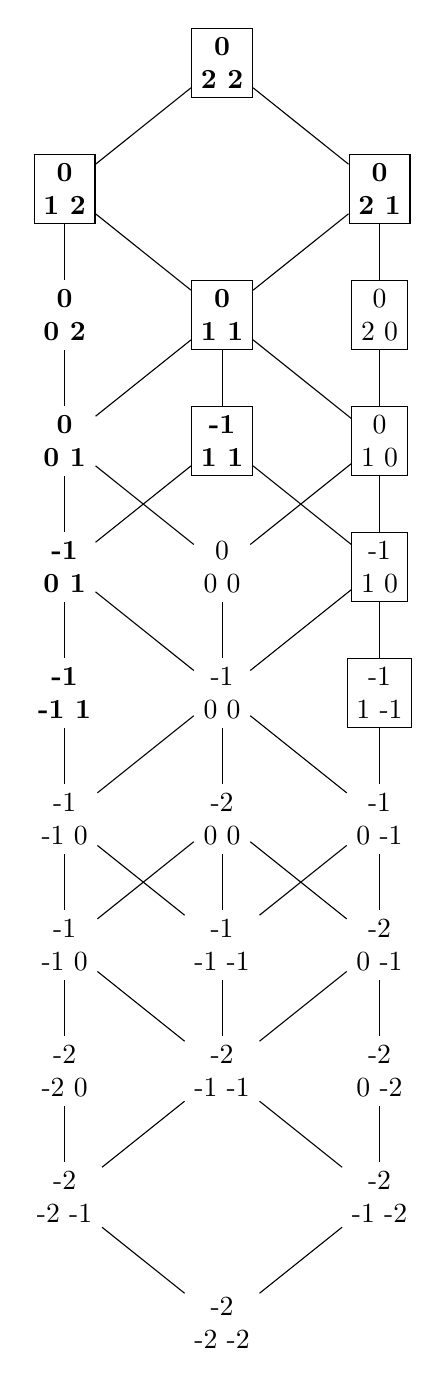
\begin{tikzpicture}[every text node part/.style={align=center}, xscale = 2, yscale = 1.6]
			\tikzstyle{fav} = [font = \bfseries]
			\tikzstyle{cond} = [draw, rectangle]
   			\path (1, 0) node[fav, cond] (022) {0\\2 2};
			\path (0, -1) node[fav, cond] (012) {0\\1 2};
			\path (2, -1) node[fav, cond] (021) {0\\2 1};
			\path (0, -2) node[fav] (002) {0\\0 2};
			\path (1, -2) node[fav, cond] (011) {0\\1 1};
			\path (2, -2) node[cond] (020) {0\\2 0};
			\path (0, -3) node[fav] (001) {0\\0 1};
			\path (1, -3) node[fav, cond] (-111) {-1\\1 1};
			\path (2, -3) node[cond] (010) {0\\1 0};
			\path (0, -4) node[fav] (-101) {-1\\0 1};
			\path (1, -4) node (000) {0\\0 0};
			\path (2, -4) node[cond] (-110) {-1\\1 0};
			\path (0, -5) node[fav] (-1-11) {-1\\-1 1};
			\path (1, -5) node (-100) {-1\\0 0};
			\path (2, -5) node[cond] (-11-1) {-1\\1 -1};
			\path (0, -6) node (-1-10) {-1\\-1 0};
			\path (1, -6) node (-200) {-2\\0 0};
			\path (2, -6) node (-10-1) {-1\\0 -1};
			\path (0, -7) node (-2-10) {-1\\-1 0};
			\path (1, -7) node (-1-1-1) {-1\\-1 -1};
			\path (2, -7) node (-20-1) {-2\\0 -1};
			\path (0, -8) node (-2-20) {-2\\-2 0};
			\path (1, -8) node (-2-1-1) {-2\\-1 -1};
			\path (2, -8) node (-20-2) {-2\\0 -2};
			\path (0, -9) node (-2-2-1) {-2\\-2 -1};
			\path (2, -9) node (-2-1-2) {-2\\-1 -2};
			\path (1, -10) node (-2-2-2) {-2\\-2 -2};
			
			\path[draw] (022) -- (012);
			\path[draw] (022) -- (021);
			
			\path[draw] (012) -- (011);
			\path[draw] (012) -- (002);
			\path[draw] (021) -- (011);
			\path[draw] (021) -- (020);

			\path[draw] (002) -- (001);
			\path[draw] (011) -- (-111);
			\path[draw] (011) -- (010);
			\path[draw] (011) -- (001);
			\path[draw] (020) -- (010);

			\path[draw] (001) -- (-101);
			\path[draw] (001) -- (000);
			\path[draw] (-111) -- (-101);
			\path[draw] (-111) -- (-110);
			\path[draw] (010) -- (000);
			\path[draw] (010) -- (-110);

			\path[draw] (-101) -- (-1-11);
			\path[draw] (-101) -- (-100);
			\path[draw] (000) -- (-100);
			\path[draw] (-110) -- (-100);
			\path[draw] (-110) -- (-11-1);

			\path[draw] (-1-11) -- (-1-10);
			\path[draw] (-100) -- (-1-10);
			\path[draw] (-100) -- (-200);
			\path[draw] (-100) -- (-10-1);
			\path[draw] (-11-1) -- (-10-1);

			\path[draw] (-1-10) -- (-2-10);
			\path[draw] (-1-10) -- (-1-1-1);
			\path[draw] (-200) -- (-2-10);
			\path[draw] (-200) -- (-1-1-1);
			\path[draw] (-200) -- (-20-1);
			\path[draw] (-10-1) -- (-1-1-1);
			\path[draw] (-10-1) -- (-20-1);

			\path[draw] (-2-10) -- (-2-20);
			\path[draw] (-2-10) -- (-2-1-1);
			\path[draw] (-1-1-1) -- (-2-1-1);
			\path[draw] (-20-1) -- (-2-1-1);
			\path[draw] (-20-1) -- (-20-2);

			\path[draw] (-2-20) -- (-2-2-1);
			\path[draw] (-2-1-1) -- (-2-2-1);
			\path[draw] (-2-1-1) -- (-2-1-2);
			\path[draw] (-20-2) -- (-2-1-2);

			\path[draw] (-2-2-1) -- (-2-2-2);
			\path[draw] (-2-1-2) -- (-2-2-2);
		\end{tikzpicture}
	\end{center}
	\caption{The lattice $>^p$ on $T$ (writing $t(b)$ then $t(d)$ $t(z)$; “fav” are bold; “cond” are rectangles)}
	\label{fig:lat}
\end{figure}

\section{Numerical examples for bound on delta}
(About \cref{th:boundDelta}.)

Consider $\alpha = 1$, $\gamma = 3$, 
thus, $P[z < b \knowing {\pprefinv}] = \frac{\delta + 10}{5 (\delta + 6)}$ and $E = \frac{4 \delta + 20}{5 (\delta + 6)} 1 + \frac{\delta + 10}{5 (\delta + 6)} 3 = \frac{7 \delta + 50}{5 \delta + 30}$; compared to $\alpha' = 0$, $\gamma' = 4$,
thus, $P[z < b \knowing {\ppref'}] = \frac{\delta + 10}{2 (\delta + 6)}$ and $E' = \frac{\delta + 10}{2 (\delta + 6)} 0 + \frac{\delta + 2}{2 (\delta + 6)} 4 = \frac{2 \delta + 4}{\delta + 6}$.
\begin{itemize}
	\item $\delta = 0$: $E - E' = \frac{5 - 2}{3} = 1$.
	\item $\delta = 1$: $E - E' = \frac{57 - 30}{35} = \frac{27}{35}$.
	\item $\delta = 2$: $E - E' = \frac{64 - 40}{40} = \frac{3}{5}$.
	\item $\delta = 10$: $E - E' = \frac{3 - 3}{2} = 0$.
\end{itemize}

Consider $\alpha = 3, \gamma = 5$ and $\alpha' = 2, \gamma' = 6$. Thus $E = \frac{6 \delta + 42}{7 \delta + 70} 3 + \frac{\delta + 28}{7 \delta + 70} 5 = \frac{23 \delta + 266}{7 \delta + 70}$ and $E' = \frac{\delta + 28}{4 \delta + 40} 2 + \frac{3 \delta + 12}{4 \delta + 40} 6 = \frac{20 \delta + 128}{4 \delta + 40} = \frac{5 \delta + 32}{\delta + 10} = \frac{35 \delta + 224}{7 \delta + 70}$.

\begin{itemize}
	\item $\delta = 0$: $E - E' = \frac{266 - 224}{70} = \frac{42}{70} = \frac{3}{5}$.
	\item $\delta = 1$: $E - E' = \frac{289 - 259}{77} = \frac{30}{77}$.
	\item $\delta = 3$: $E - E' = \frac{335 - 329}{98} = \frac{6}{98} = \frac{3}{49}$.
	\item $\delta = 4$: $E - E' = \frac{358 - 364}{98} = \frac{-6}{98} = \frac{-3}{49}$.
	\item $\delta = 5$: $E - E' = \frac{381 - 399}{105} = \frac{-18}{105} = \frac{-6}{35}$.
\end{itemize}

\section{Best possible number of edges}
Assume we are the luckiest possible: we can choose the orientation of edges (the answers to questions) so as to maximise the number of resulting edges.

Define the \emph{original graph} as the graph $G$ containing the edge $(a, b)$ iff the question $a \relq b$ was asked and answered with $a > b$. Consider $k < n$. After $k$ questions, $G$ has $k$ edges at best.
The following proposition shows that to maximise the number of edges, it is necessary and sufficient to choose any $k + 1$ vertices and connect them. Note that any graph $G$ with $k$ edges can be uniquely decomposed into components having $k_1$, $k_2$, … edges, with $\sum_i k_i = k$ (in a component, there is a non-oriented path linking any two vertices of the component, and any two components are disconnected).
\begin{proposition}
	Let $G = (\allalts, E)$ be an oriented acyclic graph (not necessarily closed transitively) composed of components having $k_1$, $k_2$, … edges, with $\sum_i k_i = k$.
	Then, its transitive closure $T_G$ has $\binom{k + 1}{2}$ edges iff there is only one component having $k$ edges; otherwise, $T_G$ has less than $\binom{k + 1}{2}$ edges.
\end{proposition}
\begin{proof}[Folklore?]
	In general, $T_G$ has at most $\sum_i \binom{k_i + 1}{2}$ edges. The claim holds because $\binom{k + 1}{2} ≥ \sum_i \binom{k_i + 1}{2}$, with equality iff there is only one component.
	Indeed, the left hand side is half of $(k + 1) k = (\sum_i k_i + 1) \sum_i k_i = (\sum_i k_i)^2 + \sum_i k_i ≥ \sum_i k_i^2 + \sum_i k_i$, with equality iff there is only one component; whereas the right hand side is half of $\sum_i (k_i + 1) k_i = \sum_i k_i^2 + \sum_i k_i$.
\end{proof}

Idea: if I have two components, I must not attach to any of them a $k+2$nd element, otherwise, I have no hope of joining the components.

Idea2: Hyp, optimal strategies with $k-1$ questions or less are all connex. Prove that opt str with $k$ questions is connex. I know that $E^k > E^{k - 1} + 1$, where $E^k$ is the expected nm of edges with opt strat.

\section{Example context}
$N$ the voters (reviewers), $\card{N} = n$; $X$ the items (articles submitted to a conference), $\card{X} = m$. $PO(X)$ the partially ordered sets over $X$. Let $Q \in PO(X)^N$ represent some partial knowledge of the voters preferences. Consider $f: PO(X)^N → \powersetz{X}$ an enlarged voting rule, that selects winning items on the basis of partial knowledge of the preferences of the voters. Define $f(Q) = \min_{x \in X} \max_{y \in X, (>_{i \in N}) \in compl(Q)} s(y, (>_{i \in N})) - s(x, (>_{i \in N}))$ as selecting the alternatives that minimize the worst regret, where $s$ is the Borda scoring rule (attributing to an alternative at a profile as many points as that alternative beats other alternatives, summed over all voters).

We are interested in asking questions so as to let the regret diminish as fast as possible.
\end{document}

